\documentclass[a4paper,11pt,twoside]{book} %,openany
%%%%%%%%%%%%%%%%%%%%%%%%%%%%%%%%%%%%%%%%%%%%%%%%%%%%%%%%%%%%%%%%%%%%%
%Packages utilisés :
\usepackage[T1]{fontenc}		%codage de caractres T1
%\usepackage{lmodern}
%\usepackage{aeguill}
\usepackage{palatino}
%\usepackage{fouriernc}
\usepackage{kpfonts}
\usepackage[utf8x]{inputenc}	%caractres accentus
\usepackage[frenchb]{babel}	%adaptation de LaTeX au français
\usepackage{amsmath}			%complement mathematique
\usepackage{amssymb}			%ajoute des symboles
	\DeclareMathOperator{\MRT}{\textit{MRT}}
	\DeclareMathOperator{\MAT}{\textit{MAT}}
	\DeclareMathOperator{\off}{\textit{off}}
%$k_{\textit{\text{12}}}$
\usepackage{array}				%Outils supplmentaires pour les tableaux
\usepackage{multicol}			%Plusieurs colonnes possibles
\usepackage{supertabular} % tableaux qui tiennent sur plusieurs pages
%\usepackage{minipage}
\usepackage{titlesec} 
\usepackage{xspace}				%Gestion des espaces
\usepackage[pdftex]{graphicx}	%inclure des graphiques
\usepackage{indentfirst} 		%indenter le premier paragraphe aprs une nouvelle section
\usepackage{latexsym}			%ajoute des symboles
\usepackage{setspace}			%Pour les Interlignes
\usepackage{makeidx}			%Pour l'index
\usepackage{vmargin}			%Definition des marges
\usepackage{pdfpages}			%Ajout de PDF
\usepackage[comma,sort&compress,super]{natbib}
\usepackage{tabularx}
\usepackage[toc]{glossaries}
\makeglossaries
%\citeindextrue
\usepackage{graphicx}
\usepackage{subcaption}
\usepackage{lscape} % Paysage
%% Numerotation continue des figures, tableaux, équations...
\usepackage{chngcntr}
\counterwithout{figure}{chapter}
\counterwithout{table}{chapter}
\counterwithout{equation}{chapter}
\usepackage{hyperref}
\titleformat{\chapter}[hang]{\bf\huge}{\thechapter}{2pc}{} 
\newcommand{\ra}[1]{\renewcommand{\arraystretch}{#1}}
%%%%%%%%%%%%%%%%%%%%%%%%%%%%%%%%%%%%%%%%%%%%%%%%%%%%%%%%%%%%%%%%%%%%%
%en tete et pied de page :
\usepackage{fancyhdr}
    \makeatletter
    \def\cleardoublepage{\clearpage\if@twoside \ifodd\c@page\else
      \hbox{}
      \thispagestyle{empty}
      \newpage
      \if@twocolumn\hbox{}\newpage\fi\fi\fi}
    \makeatother
\fancyhead{}
\fancyhead[L]{\rightmark}	%calle gauche le titre de la section courante en tete de page
\fancyfoot[C]{\thepage}		%centre LE numero de page en pied de page
\iffloatpage{\pagestyle{empty}}{\pagestyle{fancy}}
\clearpage{\pagestyle{empty}\cleardoublepage}
%%%%%%%%%%%%%%%%%%%%%%%%%%%%%%%%%%%%%%%%%%%%%%%%%%%%%%%%%%%%%%%%%%%%%
%profondeur de numerotation (1.2.1..) :
\setcounter{tocdepth}{5}
\setcounter{secnumdepth}{5}
%%%%%%%%%%%%%%%%%%%%%%%%%%%%%%%%%%%%%%%%%%%%%%%%%%%%%%%%%%%%%%%%%%%%%
%Definition cmd :
%center verticalement dans une page
\newenvironment{vcenterpage}
{\newpage\vspace*{\fill}}
{\vspace*{\fill}\par\pagebreak}
\makeindex
%%%%%%%%%%%%%%%%%%%%%%%%%%%%%%%%%%%%%%%%%%%%%%%%%%%%%%%%%%%%%%%%%%%%%
%DEBUT DU DOCUMENT
\begin{document}
\newglossaryentry{5-FU}{name=5-FU,sort=aaa, description=5-fluorouracile}
\newglossaryentry{AUC}{name={\textit{AUC}},sort=auc, description=Aire sous la courbe des concentrations en fonction du temps (\textit{Area under the concentration-time versus curve})}
\newglossaryentry{AUMC}{name={\textit{AUMC}},sort=aumc, description=Moment d'ordre 1 de la courbe des concentrations en fonction du temps (\textit{Area under the first moment of the concentration versus time curve})}
\newglossaryentry{alpha}{name={\ensuremath{\alpha}},sort=alpha, description=Pente de décroissance de la phase de distribution d'un modèle bi-compartimentale}
\newglossaryentry{beta}{name={\ensuremath{\beta}},sort=beta, description=Pente de décroissance de la phase d'élimination d'un modèle bi-compartimental}
\newglossaryentry{ADCC}{name=ADCC, description=Cytotoxicité à médiation cellulaire dépendante des anticorps (\textit{Antibody-dependent cell-mediated cytotoxicity}}
\newglossaryentry{NPDE}{name=NPDE, description=Distribution normalisée des résidus (\textit{Normalized prediction distribution error})}
\newglossaryentry{IV}{name={\textit{IV}}, description=Intra-veineuse (administration)}
\newglossaryentry{EV}{name={\textit{EV}}, description=Extra-vasculaire (administration)}

 
%%%%%%%%%%%%%%%%%%%%%%%%%%%%%%%%%%%%%%%%%%%%%%%%%%%%%%%%%%%%%%%%%%%%%
%Propiete du document :
\hypersetup{
pdfauthor = {Nicolas Azzopardi},
pdftitle = {Apport de la modélisation pharmacocinétique à l'étude de la variabilité de réponse aux anticorps monoclonaux antitumoraux : Application au cetuximab},
pdfkeywords = {anticorps monoclonaux}{cetuximab},%{ELISA}{pharmacocinétique}{relation dose-réponse}{survie sans progression}{polymorphisme génétique}{récepteurs Fc}, 
pdfsubject = {Thèse soutenue le 7 décembre 2011},
hidelinks
}
%%%%%%%%%%%%%%%%%%%%%%%%%%%%%%%%%%%%%%%%%%%%%%%%%%%%%%%%%%%%%%%%%%%%%
%Page de garde :
\thispagestyle{empty}

\setmarginsrb{25mm}{0mm}{20mm}{0mm}{0mm}{0mm}{0mm}{0mm}

\begin{tabular}{ p{3cm} p{9cm} p{3cm}}
	\begin{minipage}{3cm}
		
\includegraphics[width=2.99cm]{./images/pucvl.png} 
	\end{minipage}
	&
	\begin{minipage}{9cm}
		\begin{center}
			\textbf{\LARGE{UNIVERSITÉ FRANÇOIS~RABELAIS DE TOURS}}
		\end{center}
	\end{minipage}
	&
	\begin{minipage}{3cm}
		
\includegraphics[width=2.99cm]{./images/ufr.png} 
	\end{minipage}
\end{tabular}
	
\vspace{1cm}
	
\begin{minipage}{16cm}
	\begin{center}
		École Doctorale SST \\ \vspace{0.2cm}
		$\ $ CNRS UMR 6239
	\end{center}
\end{minipage}
	
\vspace{.5cm}
	
\begin{minipage}{16cm}
	\begin{center}
		\LARGE \textbf{THÈSE} \normalsize présentée par : \\ \vspace{0.2cm}
		\large \textbf{Nicolas AZZOPARDI}\\ \vspace{0.2cm}
		soutenue le : 7 décembre 2011
	\end{center}
\end{minipage}
	
\vspace{.5cm}
	
\begin{minipage}{16cm}
	\begin{center}
		pour obtenir le grade de : Docteur de l'Université François Rabelais \\ \vspace{0.2cm}
		Discipline/ Spécialité : Sciences de la Vie et de la Santé $/$ Pharmacologie
	\end{center}
\end{minipage}
	
\vspace{0.3cm}

\fbox{
	\begin{minipage}{16cm}
		\vspace{0.5cm}
		\begin{center}
			\Huge \textbf{Apport de la modélisation pharmacocinétique à l'étude de la variabilité de réponse aux anticorps monoclonaux antitumoraux: Application au cetuximab}%\\ %\vspace{0.2cm}
		\end{center}
		\vspace{0.3cm}
	\end{minipage}
}

\vspace{1cm}
%\begin{spacing}{1.4}
		 
\textsc{\large THÈSE dirigée par : } $\ $ \vspace{0.2cm}\\ 
\begin{tabular}{l p{2cm} p{8cm}}
	\textsc{M. PAINTAUD}  Gilles & $\ $ &  Professeur, Université François Rabelais, TOURS\\
\end{tabular}

\vspace{0.3cm}

\textsc{JURY : }  $\ $ \vspace{0.2cm} \\
\begin{tabular}{l  p{10cm}}
	\textsc{M. BÉLLISSANT}  Éric &  Professeur, Université de RENNES~1\\
	\textsc{MME. BOISDRON-CELLE}  Michèle &   HDR, Chef de département, Centre Paul Papin, ANGERS\\
	\textsc{M. CALAIS}  Gilles &   Professeur, Université François Rabelais, TOURS\\
	\textsc{M. COUET}  William &   Professeur, Université de POITIERS\\
	\textsc{M. LECOMTE}  Thierry &   Professeur, Université François Rabelais, TOURS\\
	\textsc{M. PAINTAUD}  Gilles &   Professeur, Université François Rabelais, TOURS\\
	\textsc{M. TOD}  Michel &   Professeur, Université Claude Bernard, LYON~1 Président du jury\\
\end{tabular}
\setlength{\voffset}{0pt}
%\end{spacing}


\thispagestyle{empty}
%%%%%%%%%%%%%%%%%%%%%%%%%%%%%%%%%%%%%%%%%%%%%%%%%%%%%%%%%%%%%%%%%%%%%
%Definition des dimensions :
\setlength{\voffset}{0pt} 			% offset vertical
\setlength{\topmargin}{0pt}			% Pas de marge en haut
\setlength{\headheight}{30pt}		% Haut de page
\setlength{\headsep}{30pt}			% Entre le haut de page et le texte
\setlength{\textheight}{620pt}		% Hauteur de la zone de texte
\setlength{\footskip}{30pt}			% Bas de page + sparation
\setlength{\hoffset}{0pt} 			% offset horizontal
\setlength{\oddsidemargin}{20pt}	% Marge gauche sur pages impaires
\setlength{\evensidemargin}{20pt}	% Marge gauche sur pages paires
\setlength{\textwidth}{420pt}		% Largeur de la zone de texte 
\setlength{\marginparsep}{1cm}		% Sparation de la marge
\setlength{\marginparwidth}{40pt}	% Largeur de note dans la marge
\parskip=3pt						% espace additionnel entre deux paragraphes
%\pagestyle{fancy}
%%%%%%%%%%%%%%%%%%%%%%%%%%%%%%%%%%%%%%%%%%%%%%%%%%%%%%%%%%%%%%%%%%%%%
%Page de remerciements :
\chapter*{Remerciements}
%\markright{\MakeUppercase{Remerciements}}

ici votre texte de remerciement...
%
%
%\begin{table*}\centering
%\ra{1.1}
%\rowcolors{1}{green}{pink}
%\begin{tabular}{@{}rrrrcrrrcrrr@{}}\toprule
%& \multicolumn{3}{c}{$w = 8$} & \phantom{abc}& \multicolumn{3}{c}{$w = 16$} &
%\phantom{abc} & \multicolumn{3}{c}{$w = 32$}\\
%\cmidrule{2-4} \cmidrule{6-8} \cmidrule{10-12}
%& $t=0$ & $t=1$ & $t=2$ && $t=0$ & $t=1$ & $t=2$ && $t=0$ & $t=1$ & $t=2$\\\midrule
%$dir=1$\\
%$c$ & 0.0790 & 0.1692 & 0.2945 && 0.3670 & 0.7187 & 3.1815 && -1.0032 & -1.7104 & -21.7969\\
%$c$ & -0.8651& 50.0476& 5.9384&& -9.0714& 297.0923& 46.2143&& 4.3590& 34.5809& 76.9167\\
%$c$ & 124.2756& -50.9612& -14.2721&& 128.2265& -630.5455& -381.0930&& -121.0518& -137.1210& -220.2500\\
%$dir=0$\\
%$c$ & 0.0357& 1.2473& 0.2119&& 0.3593& -0.2755& 2.1764&& -1.2998& -3.8202& -1.2784\\
%$c$ & -17.9048& -37.1111& 8.8591&& -30.7381& -9.5952& -3.0000&& -11.1631& -5.7108& -15.6728\\
%$c$ & 105.5518& 232.1160& -94.7351&& 100.2497& 141.2778& -259.7326&& 52.5745& 10.1098& -140.2130\\
%\bottomrule
%\end{tabular}
%\caption{Caption}
%\end{table*} %\clearpage{\pagestyle{empty}\cleardoublepage}
%%%%%%%%%%%%%%%%%%%%%%%%%%%%%%%%%%%%%%%%%%%%%%%%%%%%%%%%%%%%%%%%%%%%%
\begin{spacing}{1.4}
%%%%%%%%%%%%%%%%%%%%%%%%%%%%%%%%%%%%%%%%%%%%%%%%%%%%%%%%%%%%%%%%%%%%%
%Les publis :
\chapter*{Publications et manuscrit}

\begin{itemize}
\item Thariat J, \textbf{Azzopardi N}, Peyrade F, Launay-Vacher V, Santini J, Lecomte T, Etienne-Grimaldi M-C, Paintaud G, Milano G.\\
\textit{Cetuximab pharmacokinetics in end-stage kidney disease under hemodialysis.}\\
Journal of Clinical Oncology. 2008 ; 26(25) : 4223-5.

\vskip2ex
\item Cézé N, Ternant D, Piller F, Degenne D, \textbf{Azzopardi N}, Dorval E, Watier H, Lecomte T, Paintaud G.\\
\textit{An enzyme-linked immunosorbent assay for therapeutic drug monitoring of cetuximab.}\\
Therapeutic Drug Monitoring. 2009 ; 31(5) : 597-601.

\vskip2ex
\item \textbf{Azzopardi N}, Lecomte T, Ternant D, Boisdron-Celle M, Piller F, Morel A, Gouilleux-Gruart V, Vignault-Desvignes C, Watier H, Gamelin E, Paintaud G.\\
\textit{Cetuximab pharmacokinetics influences progression-free survival of metastatic colorectal cancer patients.}\\
Clinical Cancer Research. 2011 ; 17(19) : 1-9.

\vskip2ex
\item \textbf{Azzopardi N}, Pointreau Y, Ternant D, Paintaud G, Lecomte T.\\
\textit{Influence of infusion intervals on cetuximab concentrations: a simulation study.}\\
Manuscrit.

\vskip2ex
\item Maillet A, Guilleminault L, Lemarié E, Lerondel S, \textbf{Azzopardi N}, Montharu J, Congy-Jolivet N, Reverdiau P, Legrain B, Parent C, Douvin D-H, Hureaux J, Courty Y, de Monte M, Diot P, Paintaud G, Le Pape A, Watier H, Heuzé-Vourc'h N.\\
\textit{The airways, a novel route for delivering monoclonal antibodies to treat lung tumors.}\\
Pharmaceutical Research. 2011 ; 28(9) : 2147-56.
\end{itemize}
 
%%%%%%%%%%%%%%%%%%%%%%%%%%%%%%%%%%%%%%%%%%%%%%%%%%%%%%%%%%%%%%%%%%%%%
%Page Resume fr et en:
\begin{vcenterpage}
\chapter*{Résumé}
%\markright{\MakeUppercase{Résumé}}
Les anticorps monoclonaux ont révolutionné le traitement de nombreuses pathologies. Cependant, leur pharmacocinétique (PK) et l'influence de leur concentration sur la réponse clinique restent mal connues. Nous avons étudié les sources de variabilité interindividuelle de la PK du cetuximab, un anticorps anti-EGFR, ainsi que l'influence de l'exposition à cet anticorps sur la réponse. Nous avons validé une méthode ELISA de dosage du cetuximab. Dans un modèle murin, nous avons étudié l'absorption pulmonaire du cetuximab. Nous avons étudié la PK du cetuximab chez un patient hémodialysé. Nous avons décrit la PK du cetuximab chez des patients traités pour cancer colorectal métastatique, à l'aide d'un modèle combinant des éliminations d'ordre 0 et 1. Enfin, nous avons identifié la clairance globale du cetuximab, paramètre pouvant être estimé précocement par la concentration résiduelle à J14, comme un facteur influençant la survie sans progression des patients. Nos travaux montrent qu'une description de la PK d'un anticorps par approche compartimentale permet d'identifier les sources de variabilité et d'étudier l'impact de la PK sur la réponse clinique.
\paragraph*{Mots clés :} anticorps monoclonaux, cetuximab, ELISA, pharmacocinétique, relation dose-réponse, survie sans progression, polymorphisme génétique, récepteurs Fc
\end{vcenterpage} 
\begin{vcenterpage}

\chapter*{Abstract}
%\markright{\MakeUppercase{Abstract}}
Monoclonal antibodies have profoundly modified the treatment of many diseases. However, their pharmacokinetics (PK) and the influence of their concentrations on the clinical response are poorly known. We studied the sources of the interindividual variability of PK of cetuximab, an anti-EGFR, and the influence of the exposure to this antibody on the response. We validated an ELISA technique to measure cetuximab concentrations. We studied the pulmonary absorption of cetuximab in a murine model. We studied cetuximab PK in a hemodialysed patient. In metastatic colorectal cancer patients, we described cetuximab PK with the help of a model combining zero- and first-order eliminations. Finally, we identified the global clearance of cetuximab, a parameter which can be estimated by residual concentration on day 14, as a factor influencing progression-free survival of the patients. Our work shows that the description of the PK of an antibody by compartmental approach allows to identify sources of variability and to study the impact of PK on the clinical response.
\paragraph*{Keywords :} monoclonal antibodies, cetuximab, ELISA, pharmacokinetics, dose-response relationship, genetic polymorphism, Fc receptors

\end{vcenterpage} 
\end{spacing}
%%%%%%%%%%%%%%%%%%%%%%%%%%%%%%%%%%%%%%%%%%%%%%%%%%%%%%%%%%%%%%%%%%%%%
%Les sommaires :
\tableofcontents% 
%L'introduction :
\begin{spacing}{1.4}
\chapter{Introduction}
%\addtitlethumb{I}{\space\Huge{\textbf{I}}}{white}{gray}{none}
\section{Principes de la modélisation pharmacocinétique}
\subsection{Généralités}
L'effet d'un médicament dépend de la dose administrée et plus généralement de sa posologie. La posologie englobe la quantité de médicament administrée, la fréquence d'administration et la voie d'administration. Si la dose est trop faible, aucun effet ne sera observé. Si la dose est trop élevée, le patient présentera des effets indésirables dose-dépendants. Entre les deux se situe un intervalle de doses permettant d'obtenir l'effet thérapeutique souhaité tout en minimisant le risque de survenue d'effets indésirables.

Les différents mécanismes intervenant \textit{in vivo} entre l'administration d'un médicament et son effet sur l'organisme peuvent être décrits de façon quantitative. Pour cela, la relation entre la dose et l'effet est généralement décrite en deux étapes, qui sont respectivement (Figure~\ref{fig:1}) :
\begin{itemize}
\item La relation entre la dose et la concentration, ou pharmacocinétique (PK).
\item La relation entre la concentration et l'effet du médicament \textit{in vivo}, ou relation pharmacocinétique-pharmacodynamique (PK-PD)
\end{itemize}

Chacune de ces deux étapes a des sources spécifiques de variabilité, inter-- et intra-individuelles. La connaissance et la description de ces facteurs de variabilité permet de comprendre les mécanismes impliqués dans l'effet des médicaments et d'envisager une adaptation individuelle de la posologie afin d'optimiser la réponse thérapeutique.

\begin{figure}[htbp]
	\centering
		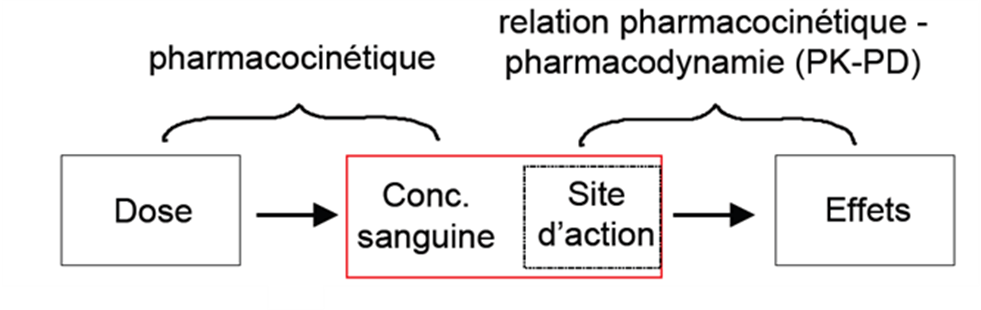
\includegraphics[width=10cm]{figures/raster/FIG_1}
	\caption{Relation dose-concentration-effet d'un médicament.}
	\label{fig:1}
\end{figure}

L'évolution des concentrations d'un médicament dans l'organisme au cours du temps dépend des modalités d'administration (forme galénique, posologie) et du devenir du médicament dans l'organisme, qui peut être décrit schématiquement par les étapes suivantes :
\begin{description}
\item[Absorption -] Une phase d'absorption existe lorsqu'un médicament est d'administré par voie extravasculaire (\gls{EV}). Seule une fraction de la dose (D) de médicament atteint alors la circulation générale. La biodisponibilité est définie à la fois par cette fraction de la dose de médicament et par la vitesse d'absorption. La fraction biodisponible est calculée par rapport à celle de la voie intraveineuse (\gls{IV}), qui est par définition de 1.
\item[Distribution -] La distribution correspond au passage du médicament dans les différents tissus et liquides biologiques de l'organisme.
\item[Élimination -] Les mécanismes d'élimination du médicament dépendent de sa nature. Dans le cas des médicaments "classiques" (petites molécules, souvent obtenues par synthèse chimique), l'élimination est due à leur métabolisme (biotransformation) ou à leur excrétion, c'est-à-dire leur élimination sous forme inchangée, par voie rénale ou biliaire notamment. Les mécanismes d'élimination des biomédicaments sont ceux des molécules endogènes dont ils sont proches. Le cas des anticorps thérapeutiques sera décrit plus loin.
\end{description}

Les études pharmacocinétiques nécessitent à la fois la mesure des concentrations de médicaments dans les milieux biologiques, notamment le sang, par une technique analytique validée, et la quantification du devenir des médicaments dans l'organisme par des méthodes mathématiques (modélisation pharmacocinétique). Nous présenterons donc dans un premier temps les différentes approches de modélisation pharmacocinétique. Nous décrirons ensuite, dans la partie 1.1.10, les différentes méthodes de mesure des concentrations sanguines des biomédicaments que sont les anticorps thérapeutiques.

\subsection{Modélisation pharmacocinétique par approche non-compartimentale}
L'objectif de l'analyse pharmacocinétique non-compartimentale est de décrire et de quantifier le devenir du médicament dans l'organisme en faisant le moins d'hypothèses possible. C'est l'approche pharmacocinétique qui est privilégiée par les agences du médicament car elle est robuste, peut être facilement vérifiée et est la plus objective. De plus, les paramètres décrits ci-après sont mesurables quel que soit l'allure des concentrations au cours du temps, pourvu qu'un nombre suffisant de prises de sang ait été réalisé.

\subsubsection{Aire sous la courbe}
L'aire sous la courbe ou \gls{AUC} (pour \textit{Area under the concentration versus time curve}) reflète l'exposition du sujet au médicament administré. Sa dimension est la suivante :

\begin{center}
\textit{Unité de concentration $\times$ Unité de temps}
\end{center}

L'\gls{AUC} est l'intégration des concentrations en fonction du temps :
\begin{equation}
\gls{AUC}(t_\infty)=\int_{0}^{t_\infty}C(t) \, dt
\label{eq:1}
\end{equation}

où $C$ est la concentration et $t$ le temps. Lors d'une administration unique, l'exposition totale du sujet est estimée par l'\gls{AUC} extrapolée à l'infini, notée $\gls{AUC}_\infty$. Dans un premier temps, l'\gls{AUC} entre les temps $t_0$ et $t_n$ est estimée par la méthode des trapèzes :
\begin{equation}
\gls{AUC}_{0 \to t_n} = \sum_{i=0}^{n-1}\left ( \frac{C_i + C_{i+1}}{2}\cdot \left ( t_{i+1}-t_i \right ) \right )
\label{eq:2}
\end{equation}
où $C_i$ est la concentration mesurée au temps $t_i$ et $t_n$ est le temps correspondant à la dernière concentration mesurée. L'\gls{AUC} entre la dernière concentration mesurée et l'infini $\gls{AUC}_{t_{n} \to \infty}$ est estimée par extrapolation de la pente de décroissance, si elle est log-linéaire. On peut démontrer que :
\begin{equation}
\gls{AUC}_{t_n \to \infty} = \frac{C_n}{\lambda_z}
\label{eq:3}
\end{equation}
où $C_n$ est la dernière concentration mesurée et $\lambda_z$ est la constante d'élimination d'ordre~1 correspondant à la pente de décroissance terminale (également appelée $k_e$ lorsqu'une seul phase de décroissance est visible). L'\gls{AUC} extrapolée à l'infini est donc calculée par :
\begin{equation}
\gls{AUC}_{0 \to \infty} =\, \gls{AUC}_{0 \to t_n} + \, \gls{AUC}_{t_n \to \infty}
\label{eq:4}
\end{equation}
La fraction extrapolée ne doit pas être trop importante, si possible inférieure à 10\% de l'\gls{AUC} totale. Lors d'administrations répétées, la mesure de l'exposition repose sur le calcul de l'\gls{AUC} à l'état d'équilibre, entre deux administrations (séparées par l'intervalle de temps $\tau$), par la méthode des trapèzes.

L'\gls{AUC} est souvent le meilleur critère pour l'étude des relations entre l'exposition et l'effet du médicament mais elle ne permet généralement pas d'étudier la relation concentration-effet individuelle et ses sources de variabilité. L'\gls{AUC} est un indice pharmacocinétique dose-dépendant et la cinétique est dite linéaire lorsque l'\gls{AUC} augmente proportionnellement à la dose.

\subsubsection{Fraction biodisponible}
Si un médicament est administré par voie~\gls{IV} et par voie~\gls{EV}, à deux moments différents suffisamment espacés pour que la première dose soit complètement éliminée, on peut calculer la fraction biodisponible $F$ :

\begin{equation}
F = \frac{\gls{AUC}_{\gls{EV}}}{\gls{AUC}_{\gls{IV}}} \cdot \frac{D_{\gls{IV}}}{D_{\gls{EV}}}
\label{eq:5}
\end{equation}

où $\gls{AUC}_{\gls{EV}}$ et $\gls{AUC}_{\gls{IV}}$ sont respectivement les \gls{AUC} après administrationé~\gls{EV} et après administration~\gls{IV}, et $D_{\gls{IV}}$ et $D_{\gls{EV}}$ sont les doses respectives de la voie~\gls{IV} et de la voie~\gls{EV}. La condition nécessaire est que la clairance ne se soit pas modifiée entre les deux études pharmacocinétiques. S'il n'y a pas de phénomènes saturables intervenant dans l'absorption, $F$ est indépendant de la dose.

\subsubsection{Temps de résidence moyen} 
La demi-vie $t_{1/2}$ est le paramètre le plus souvent utilisé pour quantifier l'élimination des médicaments. C'est le temps nécessaire pour que la concentration du médicament diminue de moitié. Lors de l'administration répétée d'un médicament, la $t_{1/2}$ permet de déterminer le temps nécessaire à l'obtention de l'état d'équilibre. Cependant, la $t_{1/2}$ ne peut être estimée s'il n'y a pas de phase log-linéaire de décroissance terminale des concentrations.

Le calcul du "temps de résidence moyen" ($\MRT$ pour \textit{Mean Residence Time}) est un autre moyen de mesurer le temps passé par un médicament dans l'organisme. Il peut être calculé quelle que soit l'allure de la cinétique des concentrations. Ce paramètre est particulièrement utile lorsqu'il s'agit de médicaments administrés par voie~\gls{EV} et ayant une absorption lente (médicament à libération prolongée ou biomédicaments administrés par voie sous-cutanée) ou irrégulière. En pratique, le $\MRT$, qui a la dimension d'un temps, est calculé après administration~\gls{IV} rapide (bolus) par :

\begin{equation}
\MRT_{\gls{IV}} = \frac{\gls{AUMC}}{\gls{AUC}}
\label{eq:6}
\end{equation}

où \gls{AUMC} (\textit{Area Under the first Moment of the concentration versus time Curve}) est le moment d'ordre~1 de la courbe des concentrations en fonction du temps. Comme l'\gls{AUC}, l'\gls{AUMC} entre les temps $t_0$ et $t_n$ peut être estimée par la méthode des trapèzes :

\begin{equation}
\gls{AUMC}_{0 \to t_n} = \sum_{i=0}^{n-1}\left ( \frac{t_i C_i + t_{i+1}C_{i+1}}{2}\cdot \left ( t_{i+1}-t_i \right ) \right )
\label{eq:7}
\end{equation}

La fraction extrapolée à l'infini est obtenue par :

\begin{equation}
\gls{AUMC}_{t_n \to \infty} = \frac{C_n \cdot t_n}{\lambda_z}+\frac{C_n }{\lambda_z^2}
\label{eq:8}
\end{equation}

Le $\MRT$ et les paramètres qui en sont dérivés ont l'avantage de pouvoir être additionnés. Par exemple, après administration extra vasculaire :
\begin{equation}
\MRT_{\gls{EV}} = \MAT + \, \MRT_{\gls{IV}}
\label{eq:9}
\end{equation}
où $\MAT$ (\textit{Mean Absorption Time}) est le temps d'absorption moyen qui reflète la vitesse d'absorption globale quelles que soient ses caractéristiques cinétiques. De plus, si $\MAT > \MRT_{\gls{IV}}$, il s'agit d'une cinétique absorption-dépendante, comme dans le cas des médicaments à libération prolongée : la vitesse d'absorption va limiter la vitesse d'élimination.

Si la décroissance terminale des concentrations est log-linéaire, la $t_{1/2}$ peut être estimée et sa relation avec le $\MRT$ est la suivante :

\begin{equation}
t_{1/2} = \ln(2)\cdot \MRT_{\gls{IV}}
\label{eq:10}
\end{equation}

\subsubsection{Clairance} 
La clairance (\gls{CL}) quantifie la capacité d'élimination du médicament par l'organisme. Elle correspond au volume de liquide biologique épuré par unité de temps. Elle a donc la dimension d'un débit volume $[L]^3.[T]^{-1}$. La clairance permet de relier à chaque instant la vitesse d'élimination à la concentration :

\begin{center}
\textit{Vitesse d'élimination = $\gls{CL} \, \times$ concentration}
\end{center}

La \gls{CL} peut être calculée, après administration~\gls{IV}, par :

\begin{equation}
\gls{CL} = \frac{D}{\gls{AUC}}
\label{eq:11}
\end{equation}

La capacité d'élimination du médicament par le patient peut donc être quantifiée quelle que soit l'allure de la courbe des concentrations en fonction du temps. S'il n'y a pas de phénomènes saturables intervenant dans l'élimination, la clairance \gls{CL} ne change pas avec la dose $D$.

\subsubsection{Volume de distribution}
Après une injection~\gls{IV}, le volume de distribution à l'état d'équilibre ($V_{SS}$) peut être estimé grâce à la clairance \gls{CL} et au temps de résidence moyen $\MRT$ par la formule suivante :

\begin{equation}
V_{SS} = \gls{CL} \cdot \MRT
\label{eq:12}
\end{equation}

\subsection{Modélisation pharmacocinétique par approche compartimentale}
Contrairement à l'approche non-compartimentale, l'approche compartimentale impose des hypothèses fortes. L'organisme est assimilé à un réseau de compartiments. Ce sont des volumes fictifs, sans réalité physiologique, dans lesquels la concentration de médicament est instantanément homogène. L'entrée et la sortie de ces compartiments étant le plus souvent liées à des phénomènes passifs, leurs vitesses peuvent être décrites par des constantes d'ordre~1, c'est-à-dire que ces vitesses sont, à chaque instant, proportionnelles à la concentration. Bien que l'approche compartimentale ne soit pas toujours applicable, elle présente les avantages suivants :
\begin{itemize}
\item elle vise une description plus mécanistique de la pharmacocinétique que l'analyse non-compartimentale.

\item elle permet, grâce à l'approche de population, d'estimer des paramètres individuels en utilisant des données "pauvres" (faible nombre de prises de sang par sujet) si le nombre de sujet est suffisamment grand.

\item Le modèle paramétrique qui en découle peut être utilisé pour prédire par simulation les concentrations attendues au cours du temps avec d'autres posologies.
\end{itemize}

\subsubsection{Modèle mono-compartimental avec élimination d'ordre~1}
Ce type de modèle pharmacocinétique est paramétré par un volume de distribution unique et par une constante d'élimination d'ordre 1 (Figure~\ref{fig:2}).

Après administration en bolus~\gls{IV}, la variation des concentrations du médicament au cours du temps est décrite par l'équation différentielle suivante :

\begin{equation}
\frac{dC}{dt} = -k_{10} \cdot C(t)
\label{eq:13}
\end{equation}

où dC/dt est la variation instantanée de la concentration en fonction du temps, $k_{10}$ la constante d'élimination d'ordre~1 de dimension [T]$^{-1}$ et $C(t)$ la concentration au temps $t$. La condition initiale de l'équation~\ref{eq:13} étant $C(0) = C_0$, c'est-à-dire la concentration sanguine extrapolée à $t = 0$, son intégration conduit à la relation :

\begin{equation}
C(t) = C_0 \cdot e^{-k_{10}\cdot t}
\label{eq:14}
\end{equation}

Dans le cas d'un modèle mono-compartimental, la demi-vie d'élimination ($t_{1/2}$) peut être estimée grâce à $k_{10}$ :

\begin{equation}
t_{1/2} = \frac{\ln(2)}{k_{10}}
\label{eq:15}
\end{equation}

Le modèle mono-compartimental peut également être exprimé en termes de "paramètres physiologiques" (Figure~\ref{fig:2}), c'est-à-dire du volume de distribution ($V$) et de la clairance systémique (\gls{CL}). Le volume de distribution est estimé par la relation suivante :

\begin{equation}
V = \frac{D}{C(0)}
\label{eq:16}
\end{equation}

\gls{CL} est relié à $k_{10}$ et à $V$ par l'équation suivante :

\begin{equation}
\gls{CL} = k_{10} \cdot V
\label{eq:17}
\end{equation}

L'équation~\ref{eq:14} s'écrit alors :

\begin{equation}
C(t) = \frac{D}{V} \cdot e^{-\frac{\gls{CL}}{V}\cdot t}
\label{eq:18}
\end{equation}

\begin{figure}[htbp]
	\centering
		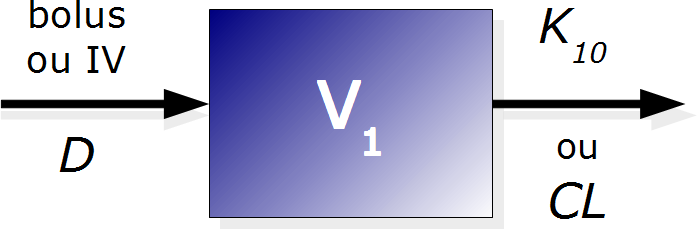
\includegraphics[width=4cm]{figures/raster/FIG_2}
	\caption[Modèle à un compartiment]{Modèle à un compartiment où $D$ est la dose de médicament administrée, $V$ le volume de distribution. L'élimination peut être codée par $k_{10}$, une constante d'élimination d'ordre~1 ou par \gls{CL}, une clairance d'élimination.}
	\label{fig:2}
\end{figure}

\subsubsection{Modèle mono-compartimental avec administration~\gls{EV}}
Lorsque le médicament est administré par voie~\gls{EV}, l'absorption peut le plus souvent être prise en compte en ajoutant un compartiment d'absorption A, sans volume, et en estimant une constante d'absorption $k_{a}$ d'ordre 1 (Figure~\ref{fig:3}). Dans le cas d'une distribution mono-compartimentale, la pharmacocinétique du médicament administré par voie~\gls{EV} peut être décrite par le système d'équations différentielles suivant :


\begin{equation}
\left| \begin{matrix}
\frac{dA}{dt} = & -k_{a}\cdot A &                & avec & A(0)&=&D\\ 
\frac{dC}{dt} = &  k_{a}\cdot A & -k_{10}\cdot C & avec & C(0)&=&0\\ 
\end{matrix}\right.
\label{eq:19}
\end{equation}

\begin{figure}[htbp]
	\centering
		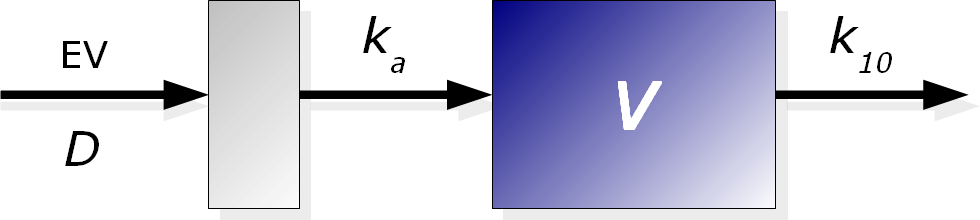
\includegraphics[width=4cm]{figures/raster/FIG_3}
	\caption[Modèle à un compartiment avec compartiment d'absorption]{Modèle à un compartiment avec compartiment d'absorption (grisé) ; $k_{a}$ et $k_{10}$ sont les constantes d'ordre~1 d'absorption et d'élimination.}
	\label{fig:3}
\end{figure}

Si le début de l'absorption est décalé par rapport au temps d'administration~\gls{EV}, comme cela est fréquemment le cas après administration orale, un temps de retard appelé \textit{lag-time} (noté $t_{lag}$) peut être pris en compte et estimé. Ce décalage de l'absorption peut également être décrit à l'aide de compartiments de transit. Ce type de modèle décrit le retard de l'absorption par le passage du médicament par une série de compartiments de transit an sans volume, avec une constante de transfert unique $k_t$.

Dans le cas d'un modèle à un compartiment, la pharmacocinétique du médicament administré par voie~\gls{EV} avec retard d'absorption peut être décrite par le système de $n+2$ équations différentielles suivant :

\begin{equation}
x
\label{eq:20}
\end{equation}

L'absorption est dans ce cas définie à la fois par la fraction biodisponible $F$ et par une constante d'absorption $k_{a}$ mais également par une constante de transfert $k_t$ et le nombre de compartiments de transit $n$. En pratique, le nombre d'équations dans le système~\ref{eq:20} est fixé par $n$. Pour trouver le nombre n de compartiments de transit qui permet au mieux de décrire l'absorption, il est donc nécessaire de faire plusieurs essais. Cette limitation peut être contournée~\citep{REF1}, en simplifiant le système d'équation~\ref{eq:20} par le système suivant si $n > 2$ :

\begin{equation}
x
\label{eq:21}
\end{equation}

Cette simplification permet d'estimer le nombre de compartiments $n$ comme un paramètre du modèle. Cependant, cette simplification ne peut être utilisée que pour les administrations uniques de médicament.

\subsubsection{Correspondance avec l'analyse non-compartimentale}
Il existe une correspondance entre les paramètres de l'analyse mono-compartimentale et les paramètres de l'analyse non-compartimentale :

\begin{equation}
\MRT_{\gls{IV}} = \frac{1}{k_{10}}
\label{eq:22}
\end{equation}


\begin{equation}
\MAT = \frac{1}{k_a}
\label{eq:23}
\end{equation}

En pratique, $k_a$ est souvent difficile à estimer, surtout si l'absorption est lente, alors que le $\MAT$ peut toujours être calculé si l'on dispose de données après voie~\gls{IV} et voie~\gls{EV}.

\subsubsection{Modèle bicompartimental avec constantes de transfert d'ordre~1}
Dans la plupart des cas, les médicaments ne sont pas instantanément distribués de façon homogène dans tout l'organisme. Le modèle bi-compartimental permet de décrire le fait que les concentrations dans deux groupes de tissus ou de fluides biologiques ne s'équilibrent pas immédiatement. Les échanges entre ces compartiments sont le plus souvent décrits par des constantes de transfert d'ordre~1. Le compartiment "central" correspond au sang et aux tissus dans lesquels les concentrations s'équilibrent rapidement avec celles du sang. Le compartiment périphérique correspond aux tissus et organes dans lesquels la concentration du médicament s'équilibre plus lentement avec celle du compartiment central. Pour des raisons d'identifiabilité, l'élimination du médicament de l'organisme est le plus souvent décrite comme se faisant à partir du compartiment central.

Comme le modèle mono-compartimental, le modèle bi-compartimental peut être paramétré de plusieurs façons :

\paragraph*{Paramétrisation à l'aide de "micro-constantes":} Après administration par voie~\gls{IV} bolus, le modèle est décrit à l'aide du volume du compartiment central ($V_1$), des constantes de distribution $k_{12}$ et $k_{21}$ (d'ordre~1) et de la constante d'élimination $k_{10}$ (Figure~\ref{fig:4}) :

\begin{equation}
\left| \begin{matrix}
\frac{dC_1}{dt} = & k_{10}\cdot C_1 &- &k_{12}\cdot C_1 & + & k_{21}\cdot C_2 & avec & C_1(0)&=&\frac{D}{V_1}\\ 
\frac{dC_2}{dt} = &                 &  &k_{12}\cdot C_1 & - & k_{21}\cdot C_2 & avec & C_2(0)&=&0 \\ 
\end{matrix}\right.
\label{eq:24}
\end{equation}

où $C_1$ et $C_2$ sont les concentrations du médicament, respectivement dans le compartiment central et le compartiment périphérique.

\paragraph*{Paramétrisation "physiologique":} Le modèle est décrit à l'aide des volumes de distribution du compartiment central et périphérique, respectivement $V_1$ et $V_2$, et des clairances systémique \gls{CL} et de distribution $Q$ (\ref{fig:5}). 

Les relations entre les micro-constantes et les constantes physiologiques sont les suivantes :

\begin{equation}
k_{10}  =  \frac{\gls{CL}}{V_1}
\label{eq:25}
\end{equation}

\begin{equation}
k_{12}  =  \frac{Q}{V_1}
\label{eq:26}
\end{equation}

\begin{equation}
k_{21}  =  \frac{Q}{V_2}
\label{eq:27}
\end{equation}

\begin{figure}[h!]
        \centering 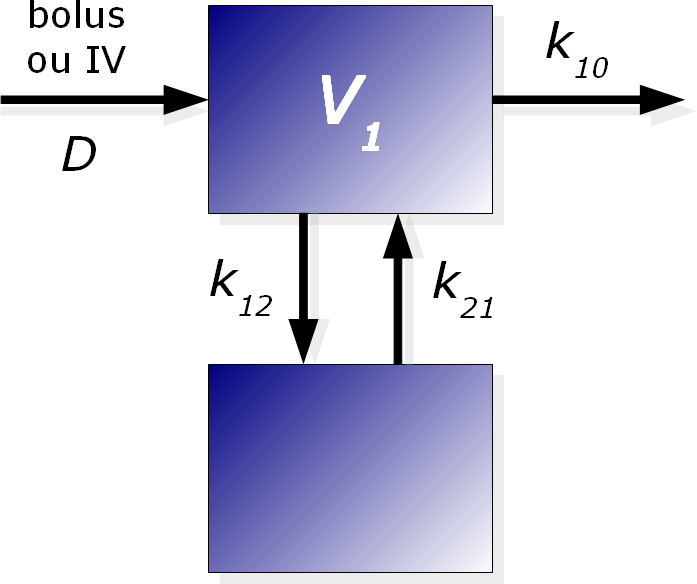
\includegraphics[width=4cm]{figures/raster/FIG_4}
        \caption[Modèle à deux compartiments (micro constantes]{Modèle à deux compartiments où $D$ est la dose de médicament administrée, $V_1$ et $V_2$ les volumes de distribution, $k_{10}$ la constante d'élimination d'ordre~1, $k_{12}$ et $k_{21}$ les constantes de distribution.}
	\label{fig:4}
        \centering 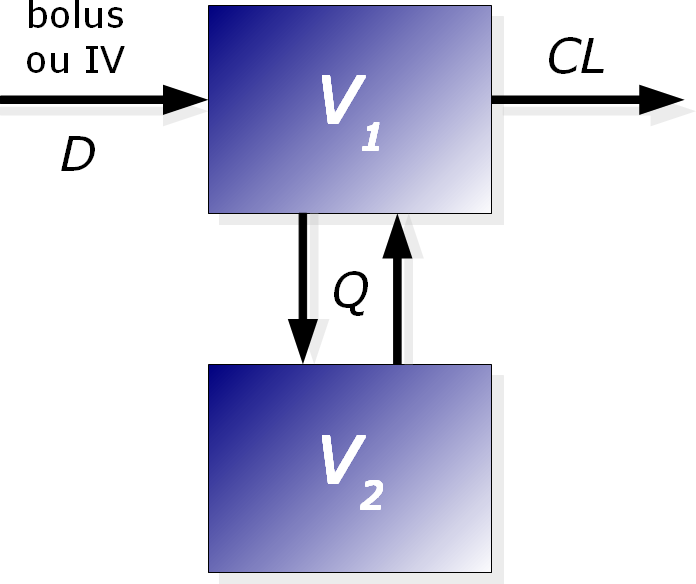
\includegraphics[width=4cm]{figures/raster/FIG_5}
        \caption[Modèle à deux compartiments (constantes "physiologiques")]{Modèle à deux compartiments où $D$ est la dose de médicament administrée, $V_1$ et $V_2$ les volumes de distribution, \gls{CL} et $Q$ les clairances d'élimination et de distribution.}
	\label{fig:5}
\end{figure}

\paragraph*{Paramétrisation à l'aide de "macro-constantes":} Celle-ci permet de faire une description graphique de l'évolution des concentrations et d'estimer les demi-vies de distribution et d'élimination. Ainsi la cinétique de décroissance des concentrations de médicament s'écrit :

\begin{equation}
C(t) = A \cdot e^{-\gls{alpha}\cdot t}+B \cdot e^{-\gls{beta}\cdot t}
\label{eq:28}
\end{equation}

où $A$ et $B$ sont respectivement les concentrations de distribution et d'élimination, extrapolées au temps $0$ ("à l'origine") par approche "graphique", analogues au $C_0$ du modèle mono-compartimental, et \gls{alpha} et \gls{beta} sont respectivement les macro-constantes de distribution et d'élimination définies par :

\begin{equation}
\gls{alpha} = \frac{1}{2}\cdot[k_{12}+k_{21}+k_{10}+\sqrt{(k_{12}+k_{21}+k_{10})^2-4\cdot k_{21}\cdot k_{10}}]
\label{eq:29}
\end{equation}

\begin{equation}
\gls{beta} = \frac{1}{2}\cdot[k_{12}+k_{21}+k_{10}-\sqrt{(k_{12}+k_{21}+k_{10})^2-4\cdot k_{21}\cdot k_{10}}]
\label{eq:30}
\end{equation}

On note que l'équation~\ref{eq:15} de calcul de la demi-vie pour le modèle mono-compartimental ne s'applique pas au modèle bi-compartimental. En revanche à l'aide des paramètres \gls{alpha} et \gls{beta}, il est possible de calculer :

\begin{equation}
t_{1/2}\gls{alpha} = \frac{ln(2)}{\gls{alpha}}
\label{eq:31}
\end{equation}
et
\begin{equation}
t_{1/2}\gls{beta}  = \frac{ln(2)}{\gls{beta}} 
\label{eq:32}
\end{equation}
qui sont respectivement les demi-vies de distribution et d'élimination~\citep{REF2}.

\subsubsection{Modèles avec élimination saturable}
Lorsque l'élimination du médicament est liée à des phénomènes actifs et que la capacité d'élimination est limitée, on parle d'élimination saturable. Les vitesses de transfert du médicament ne sont alors plus proportionnelles à la concentration et à forte concentration, la vitesse d'élimination est à sa valeur maximale. Ce phénomène peut être décrit par différents modèles mécanistiques : modèle d'élimination liée à la cible (TMDD pour \textit{Target Mediated Drug Disposition}), modèle avec élimination de type Michaelis-Menten ou encore modèle avec constante d'élimination d'ordre~0. 

L'élimination saturable des médicaments "classiques", généralement liée à une saturation du métabolisme hépatique, peut être décrite par une équation de type Michaelis-Menten, le métabolisme étant limité par la quantité d'enzyme présente dans l'organisme. Si la vitesse d'élimination est la plupart du temps à sa valeur maximale, la description mathématique de celle-ci peut être simplifiée en utilisant une constante d'élimination d'ordre~0.
\paragraph{Modèle mécanistique TMDD} Le modèle mécanistique TMDD a été développé pour décrire les pharmacocinétiques de médicaments dont la distribution et/ou l'élimination sont influencées par la fixation sur leur cible~\citep{REF3}. Ce modèle est fréquemment utilisé pour les anticorps monoclonaux~\citep{REF4}. La fixation peu réversible des anticorps sur leur cible est en effet souvent suivie de leur élimination. S'il s'agit d'un antigène membranaire, une internalisation du complexe antigène-anticorps ou une cytolyse peuvent être observées. S'il s'agit d'un antigène circulant, un complexe immun est formé puis dégradé par les macrophages. Lorsque la cible est en quantité limitée par rapport à la concentration d'anticorps, la fraction de l'élimination de l'anticorps due à l'interaction avec la cible est saturable.

Un modèle pharmacocinétique de type TMDD est une interprétation mécanistique précise de l'interaction entre le médicament et sa cible au cours du temps (Figure~\ref{fig:6}). Les variations de concentration de médicament, de quantité de cible et de complexe médicament-cible sont décrites par le système d'équations différentielles suivant :

\begin{equation}
x
\label{eq:33}
\end{equation}

\begin{figure}[htbp]
	\centering
		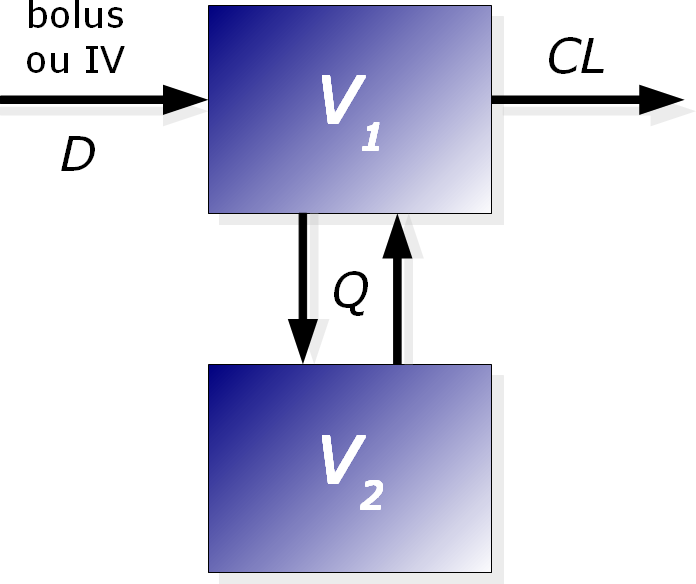
\includegraphics[width=10cm]{figures/raster/FIG_5}
	\caption[Représentation d'un modèle TMDD]{Représentation d'un modèle TMDD où $C$ est la concentration du médicament libre, $R$ est la cible libre et $RC$ est le complexe cible-médicament.}
	\label{fig:6}
\end{figure}

Le médicament sous forme libre, de concentration $C$, se lie à une quantité de cible libre $R$ avec une constante d'association $k_{on}$. Cette constante est d'ordre~2 car l'association dépend à la fois de la concentration $C$ et de la quantité de récepteur $R$. Cette association forme un complexe médicament-cible $RC$. Le complexe $RC$ peut soit se dissocier avec une constante de dissociation d'ordre~1 $k_{off}$ (qui est très faible pour les anticorps) soit être internalisé ou dégradé avec une constante d'ordre~1 $k_{int}$. Comme indiqué dans le système d'équations~\ref{eq:33}, le modèle peut également prendre en compte le fait que les cibles libres sont synthétisées avec une constante d'ordre~0 $k_{syn}$ et dégradées indépendamment de l'effet du médicament, avec une constante de dégradation d'ordre~1 $k_{deg}$~\citep{REF3}.

Un tel modèle doit être couplé à un modèle compartimental classique qui décrit les phénomènes d'absorption, de distribution et d'élimination du médicament qui ne sont pas liés à la cible. Dans ce cas, $C$ représente la concentration dans le compartiment central.

\paragraph{Élimination de type Michaelis-Menten} L'équation de Michaelis-Menten a été initialement proposée pour décrire la saturation de la cinétique enzymatique~\citep{REF5}. Elle est maintenant couramment utilisée pour décrire, entre autres, la cinétique d'élimination saturable de certains médicaments. D'après le modèle de Michaelis-Menten, ce type d'élimination est décrit par l'équation différentielle suivante :

\begin{equation}
\frac{dC}{dt}=-\frac{V_{max}\cdot C}{k_M + C}
\label{eq:34}
\end{equation}
où $V_{max}$ est la vitesse maximale d'élimination du médicament et $k_M$ est la constante dite de Michaelis, qui correspond à la concentration de médicament pour laquelle la vitesse d'élimination est égale à la moitié de $V_{max}$ (Figure~\ref{fig:7}).

\begin{figure}[htbp]
	\centering
		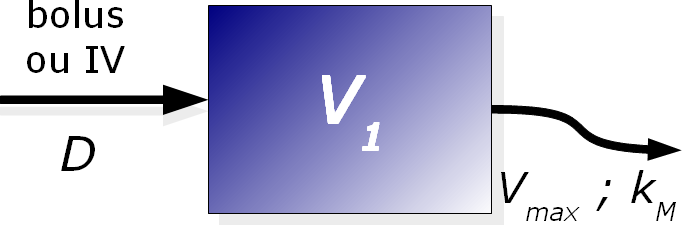
\includegraphics[width=4cm]{figures/raster/FIG_7}
	\caption{Modèle à un compartiment avec élimination de type Michaelis-Menten.}
	\label{fig:7}
\end{figure}

Un tel type d'élimination peut être considéré comme une simplification d'un modèle TMDD sous deux conditions :
\begin{itemize}
\item L'affinité du médicament pour sa cible est très forte (c'est-à-dire : $k_{on} >> k_{off}$).
\item La quantité totale de cible $R_{tot} =  R + RC$ reste constante au cours du temps.
\end{itemize}
Dans ces conditions, les paramètres de Michaelis-Menten sont définis par : $V_{max} = k_{int}\cdot R_{tot}\cdot V$ où $V$ est le volume de distribution du médicament et par $k_M = k_{off} /k_{on}$~\citep{REF4, REF6}.
\paragraph{Élimination d'ordre~0} Ce modèle est le plus simple pour décrire une élimination saturable. L'élimination n'est pas dépendante de la concentration et la vitesse d'élimination (quantité de médicament éliminée par unité de temps) est constante (Figure~\ref{fig:8}). Ce type d'élimination est décrit par l'équation différentielle suivante :

\begin{equation}
\frac{dC}{dt}=-k_0
\label{eq:35}
\end{equation}

où $k_0$ est une constante d'ordre~0, la vitesse d'élimination étant indépendante de la concentration.

L'élimination d'ordre~0 est un cas particulier de l'élimination de type Michaelis-Menten, correspondant à des concentrations de médicaments $>> k_M$. Dans ce cas, $k_M$ n'est pas identifiable et $k_0 \approx V_{max}$.

\begin{figure}[htbp]
	\centering
		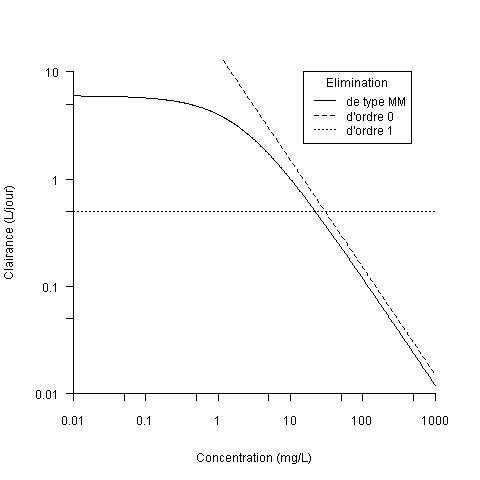
\includegraphics[width=10cm]{figures/raster/FIG_8}
	\caption[Clairance du médicament en fonction de sa concentration.]{Clairance du médicament en fonction de sa concentration. En trait plein, élimination de type Michaelis-Menten ; en trait discontinus, élimination d'ordre~0 (indépendante de la concentration) ; en pointillés, élimination d'ordre~1 (proportionnelle à la concentration).}
	\label{fig:8}
\end{figure}

\subsection{Relation dose-concentration-effet d'un médicament}
La relation dose-effet ou dose-réponse décrit l'augmentation de l'effet en fonction de la dose. La variabilité interindividuelle de cette relation est due à la fois à la variabilité de la relation dose-concentration (pharmacocinétique, traitée plus haut) et à la variabilité de la relation concentration-effet. La relation concentration-effet observée dans un modèle in vitro peut être décrite par des équations sigmoïdes $E_{max}$ ou sigmoïdes $I_{max}$ (inhibition de l'effet). Cependant, ces équations simples sont souvent insuffisantes pour décrire la relation concentration-effet \textit{in vivo}. Notamment, lorsque l'effet est retardé par rapport à la concentration, la représentation de la courbe de l'effet en fonction de la concentration fait apparaître une hystérèse antihoraire (si l'effet augmente avec la concentration). Ce phénomène peut être décrit grâce à l'utilisation d'un compartiment d'effet ou d'un modèle indirect.

Les sources de variabilité de la relation concentration-effet sont multiples. Elles incluent notamment les facteurs génétiques, le stade de la maladie et les traitements associés~\citep{REF7}.

L'étude des sources de variabilité interindividuelle de la relation concentration-effet des médicaments nécessite une mesure quantitative de l'effet, ce qui repose habituellement sur l'utilisation de biomarqueurs. Un biomarqueur est une caractéristique qui est mesurée et évaluée en tant qu'indicateur de processus biologiques normaux, de processus pathogéniques, ou de réponses pharmacologiques. Dans le cas des anticorps utilisés dans les maladies inflammatoires, tels que les anti-TNF$\alpha$, les biomarqueurs utilisés sont par exemple la vitesse de sédimentation, la protéine C-réactive (\gls{CRP}) et les scores d'activité de la maladie (DAS28, BASDAI, etc.).

En cancérologie, il existe de nombreux marqueurs biochimiques, tels que le CA19.9 ou l'ACE, mais leur relation avec la réponse thérapeutique est complexe. La variation de la taille des tumeurs, exprimée par le critère RECIST, qui est devenu le principal critère de réponse, reste la plus pertinente. Cependant, il existe une forte variabilité interindividuelle de l'évolution de ce critère, ce qui rend sa modélisation difficile en pratique. Pour cela, la réponse, qui est une catégorisation des variations du critère RECIST, est souvent utilisée  (Tableau~\ref{tab:1} ci-après). 

\begin{table}[!ht]
  \centering
  \caption[Correspondance entre la réponse objective et le critère RECIST]{Correspondance entre la réponse objective et le critère RECIST : (A) : Entre les réponses objectives sur les lésions cibles et les variations du critère RECIST mesuré sur ces lésions. (B) : Entre les réponses objectives sur les lésions non cibles et la variation du nombre 
et/ou de la taille de ces lésions.}
    \begin{tabular}{l p{4cm} c p{5cm}}
       &  &  &  \\
             \textbf{A} & \textbf{} & \textbf{} & \textbf{} \\
      \hline
      \hline
       & Réponse objective sur les lésions cibles & abréviation & Critère \\
       & Réponse complète & CR & disparition de toutes les lésions cibles \\
       & Réponse partielle & PR & diminution d'au moins 30 \% du RECIST \\
       & Stabilité tumorale & SD & diminution de moins de 30 \% \\
       &  &  & ou augmentation de moins de 20 \% du RECIST \\
       & Progression tumorale & PD & augmentation d'au moins 20 \% du RECIST \\
      \hline
       &  &  &  \\
     \textbf{B} &  &  &  \\
       \hline
       \hline
      & Réponse objective sur les lésions non cibles & abréviation & Critère \\
       & Réponse complète & CR & disparition de toutes les lésions \\
       & Stabilité tumorale & SD & persistance de une ou de plusieurs lésions \\
       & Progression tumorale & PD & apparition de une ou de plusieurs nouvelles lésions \\
      \hline
    \end{tabular}
  \label{tab:1}
\end{table}
Le but d'un traitement anticancéreux est de maximiser le temps pendant lequel la maladie ne progresse pas. Ce temps est appelé le temps de survie sans progression (PFS pour \textit{progression-free survival}).

\subsection{Principes de l'estimation des paramètres d'un modèle pharmacocinétique}
Avant d'estimer les paramètres d'un système d'équations différentielles, il est important de s'assurer de leur identifiabilité ; c'est-à-dire qu'à partir des données expérimentales, le système d'équations admet une solution unique pour chaque paramètre. Par exemple, la pharmacocinétique d'un médicament administré de façon régulière en bolus~\gls{IV} avec un intervalle de temps $\tau$ ne peut être décrite par un modèle à deux compartiments (équation~\ref{eq:24}) si les concentrations disponibles ne sont que des concentrations résiduelles (avant réinjection). En effet, dans ce cas, les paramètres correspondant au compartiment périphérique $Q$ et $V_2$ ne sont généralement pas identifiables.

La modélisation pharmacocinétique s'inscrit dans le cadre de la régression non-linéaire sur mesures répétées. Comme pour de nombreux types de modélisation, la qualité d'un modèle pharmacocinétique est quantifiée par la "-2ln-vraisemblance" ($-2LL$) ou par le critère d'information d'Akaïke (AIC). La $-2LL$ est couramment appelée fonction objective (FO). Les paramètres sont estimés en minimisant la FO. 

L'équilibre entre complexité du modèle et ajustement des données prédites et observées doit être recherché. Un modèle complexe peut fournir un ajustement très précis entre les données, mais ses paramètres risquent de ne pas être identifiables. Ainsi, pour des valeurs de fonction objective non significativement différentes, le modèle le plus simple doit être privilégié. Par exemple, un modèle à deux compartiments n'est justifié que s'il permet d'obtenir une valeur de fonction objective significativement inférieure à celle d'un modèle à un compartiment.

La modélisation pharmacocinétique peut être réalisée par approche individuelle ou par approche de population. 

\subsubsection{Approche individuelle}
L'approche individuelle consiste à étudier le profil des concentrations sanguines du médicament chez chaque sujet, indépendamment des autres sujets. Elle permet une description précise pour chaque sujet, même si la variabilité interindividuelle des paramètres estimés est grande. Cette approche nécessite cependant un grand nombre de données pour chaque sujet.

\subsubsection{Approche de population}
A l'origine, l'approche de population a été proposée pour analyser des données "pauvres" (faible nombre de données par patient) et "hétérogènes" (posologies et temps d'observation différents d'un patient à l'autre) car provenant de larges cohortes de patients~\citep{REF8}. Elle est maintenant de plus en plus utilisée pour l'analyse de données "riches" recueillies dans le cadre d'études pharmacocinétiques cliniques. Cette approche est recommandée par la Food and Drug Administration (FDA) pour l'obtention de l'autorisation de mise sur le marché (\gls{AMM})~\citep{REF9}.

L'analyse pharmacocinétique de population prend en compte l'ensemble des individus inclus dans l'étude et permet donc d'utiliser l'information de chaque sujet pour estimer des paramètres moyens dans la population considérée.

La modélisation de population s'inscrit dans le cadre des modèles non-linéaires à effets mixtes sur mesures répétées~\citep{REF10}. Les modèles de population sont également appelés "hiérarchiques" car ils incluent plusieurs niveaux de variabilité. A chacun de ces niveaux correspond un modèle descriptif, comme décrit ci-dessous.

\paragraph*{Modèle structural :} Pour la pharmacocinétique, il s'agit du modèle qui relie la concentration au temps. La fonction qui relie les deux variables comporte les paramètres pharmacocinétiques : volume de distribution, clairance, constantes de transfert, etc. Le modèle structural s'écrit :

\begin{equation}
x
\label{eq:36}
\end{equation}

où $Y$ est la variable étudiée, $Y_{ij,pred}$ est la valeur prédite par le modèle pour le sujet~$i$ et la répétition~$j$ et $\varphi_i$ sont les paramètres du sujet~$i$.

Exemple : Après une dose unique et d'après l'équation~\ref{eq:18}, pour un modèle pharmacocinétique mono-compartimental avec élimination d'ordre~1, l'équation~\ref{eq:36} peut s'écrire :

\begin{equation}
x
\label{eq:37}
\end{equation}

où $C_{ij,pred}$ est la concentration prédite par le modèle pour le sujet $i$ au temps de prélèvement $j$, $D_i$, $V_i$ et $\gls{CL}_i$ sont respectivement la dose administrée au sujet $i$, le volume de distribution et la clairance du sujet $i$.

\paragraph*{Modèle d'erreur interindividuelle :} Il décrit la variabilité interindividuelle des sujets, c'est-à-dire l'écart entre les paramètres de population et les paramètres individuels estimés. Ce modèle s'écrit :
\begin{equation}
x
\label{eq:38}
\end{equation}
où $\varphi_k$ est le modèle d'erreur interindividuelle utilisé pour décrire la variabilité des valeurs individuelles $\theta_{ki}$ du paramètre de population $\theta_k$ et  $\eta_{ki}$ quantifie la différence individuelle du sujet $i$ par rapport à $\theta_k$. On suppose la distribution des $\eta_{ki}$ normale et centrée, telle que :

\begin{equation}
x
\label{eq:39}
\end{equation}

où $\omega_k^2$ est la variance interindividuelle du paramètre.

Pour décrire la variabilité interindividuelle des paramètres, plusieurs modèles peuvent être utilisés :

\begin{itemize}
\item Modèle additif :
\begin{equation}
x
\label{eq:40}
\end{equation}

\item Modèle proportionnel :
\begin{equation}
x
\label{eq:41}
\end{equation}

\item Modèle exponentiel :
\begin{equation}
x
\label{eq:42}
\end{equation}
 
\end{itemize}

En pratique, le modèle exponentiel est le plus utilisé car c'est le seul qui ne peut pas donner de valeurs d'$\theta_{ki}$ nulles ou négatives. Surtout, le rapport de deux lois log-normales (issue d'un modèle exponentiel) suit également une loi log-normale tandis que le rapport de deux lois normales suit une loi de Cauchy (aussi appelée loi de Lorentz) qui n'admet ni espérance, ni écart-type. Ceci serait par exemple problématique pour établir des relations entre micro constantes et constantes physiologiques (équations~\ref{eq:25}-\ref{eq:27}). 

Si aucune variabilité interindividuelle n'est estimée,

\begin{equation}
\theta_{ki} = \theta_k
\label{eq:43}
\end{equation}

Pour chaque individu $i$, la valeur $\theta_{ki}$ du $k$éme paramètre est donc égale à $\theta_k$.

\paragraph*{Modèle de covariables :} une covariable est une caractéristique individuelle qualitative ou quantitative avec laquelle la valeur d'un paramètre est significativement reliée. Les covariables sont souvent des facteurs démographiques (âge, taille, poids, sexe, surface corporelle, etc.) ou biologiques (clairance de la créatinine, numération sanguine, etc.). L'intérêt d'inclure une covariable dans l'analyse pharmacocinétique est d'expliquer une partie de la variabilité interindividuelle d'un paramètre. Si cette inclusion a une influence significative sur la fonction objective (\textit{cf.} partie 3.2.4 page 63), elle peut réduire la variabilité interindividuelle d'un paramètre et, dans une moindre mesure, l'erreur résiduelle du modèle (\textit{cf.} \textit{infra}). Dans le modèle final, la covariable devient ainsi un facteur explicatif et prédictif de la variabilité de la pharmacocinétique du médicament. Par exemple, si le volume de distribution d'un médicament augmente avec le poids, le poids est un facteur prédictif d'exposition à ce médicament, car on peut s'attendre à trouver, pour une même dose injectée, des concentrations de médicament d'autant plus faibles que le poids des patients augmente. 

Si aucune covariable n'est ajoutée au modèle interindividuel, $\theta_k$ s'écrit :

\begin{equation}
x
\label{eq:44}
\end{equation}

où $\theta_{k,TV}$ est la valeur "typique" (\textit{typical value}) du paramètre $k$, dans la population. Si une covariable $m$ est ajoutée au modèle interindividuel, $\theta_{k,TV}$ s'écrit :

\begin{equation}
x
\label{eq:45}
\end{equation}

où $g$ est le modèle de covariables et $z_{kmi}$ est la valeur de la covariable $m$ propre au sujet $i$ et au paramètre $k$.

Exemple : Pour un modèle interindividuel exponentiel, la clairance du sujet $i$ s'écrit :

\begin{equation}
\gls{CL}_i
\label{eq:46}
\end{equation}

Si $\gls{CL}_{TV}$ est influencée par la surface corporelle (BSA pour \textit{body surface area}) du patient (Figure~\ref{fig:9}), la valeur typique de \gls{CL} peut s'écrire :

\begin{equation}
x
\label{eq:47}
\end{equation}

où \gls{CL} est la valeur de population de la clairance, $\beta_{BSA,\gls{CL}}$ est une constante, $BSA_i$ la surface corporelle du patient $i$ et $BSA_{med}$ la surface corporelle médiane de la population. Pour un modèle interindividuel exponentiel, la clairance $\gls{CL}_i$ du sujet $i$ s'écrit donc :

\begin{equation}
x
\label{eq:48}
\end{equation}

\begin{figure}[htbp]
	\centering
		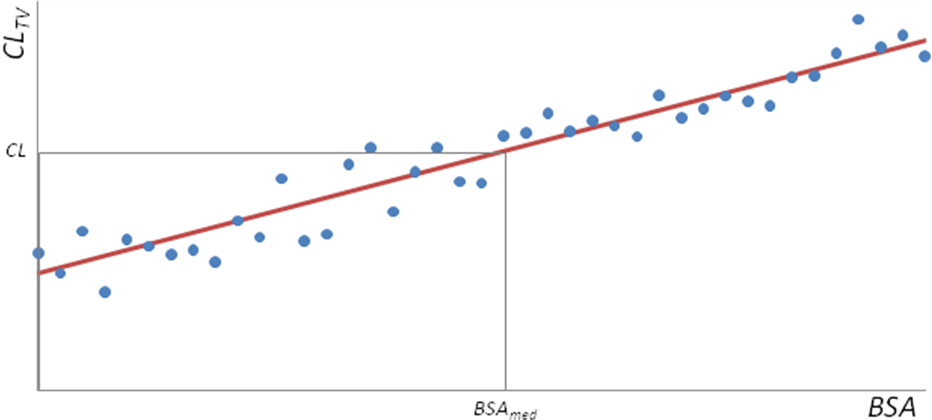
\includegraphics[width=10cm]{figures/raster/FIG_9}
	\caption[Modèle de covariable.]{Modèle de covariable. Exemple d'une relation linéaire entre la clairance systémique d'un médicament et la surface corporelle (BSA). Les points bleus représentent les valeurs individuelles. $TV$ : \textit{Typical Value} ; med : Valeur médiane.}
	\label{fig:9}
\end{figure}

Une covariable est retenue pour être testée sur un paramètre du modèle structural si des arguments biologiques ou bibliographiques le justifient (ex. : influence du poids sur le volume de distribution $V_1$) et si elle n'est pas trop fortement corrélée (|coefficient de corrélation| > 0,3) avec une autre covariable d'intérêt (ex. : la surface corporelle avec le poids)~\citep{REF11}. Si ces conditions sont respectées, la covariable est appelée covariable d'intérêt. La significativité de l'influence des covariables d'intérêt sur les paramètres est classiquement testée par une procédure pas à pas ascendante puis pas à pas descendante (\textit{cf.} méthode). Une autre procédure de test de la significativité des covariables d'intérêt consiste à tester toutes les covariables d'intérêt en même temps (\textit{Full covariate model}). La significativité est contrôlée par un test de Wald~\citep{REF12}. Cette procédure, qui nécessite cependant une plus grande puissance de calcul, est encore peu utilisée.

A la fin de ces procédures, le modèle obtenu comporte uniquement les covariables qui influencent significativement les paramètres.

\paragraph*{Modèle d'erreur résiduelle :} Malgré l'utilisation d'un modèle de variabilité interindividuel et d'un modèle de covariables, il reste toujours un écart "résiduel", appelé résidu, entre la valeur d'une concentration observée et celle de la concentration prédite (Figure~\ref{fig:10}). Le modèle d'erreur résiduelle permet de décrire la distribution des résidus. L'équation générale du modèle d'erreur résiduelle s'écrit :

\begin{equation}
x
\label{eq:49}
\end{equation}

où $Y_{ij,obs}$ est la $j$ème valeur observée (ici, une concentration) pour le sujet $i$, $\zeta$ est le modèle d'erreur résiduelle et $\varepsilon_{ij}$ est une variable aléatoire. On suppose que $\varepsilon_{ij} \sim \mathcal{N}(0 ; \sigma^2)$ où $\sigma^2$ est la variance résiduelle. Comme pour la variabilité interindividuelle, plusieurs modèles d'erreur résiduelle peuvent être utilisés (Figure~\ref{fig:10}) :
\begin{itemize}
\item Modèle additif :
\begin{equation}
x
\label{eq:50}
\end{equation}

\item Modèle proportionnel :
\begin{equation}
x
\label{eq:51}
\end{equation}

\item Modèle mixte :
\begin{equation}
x
\label{eq:52}
\end{equation}

\item Modèle exponentiel :
\begin{equation}
x
\label{eq:53}
\end{equation}

\end{itemize}

\begin{figure}[htbp]
	\centering
		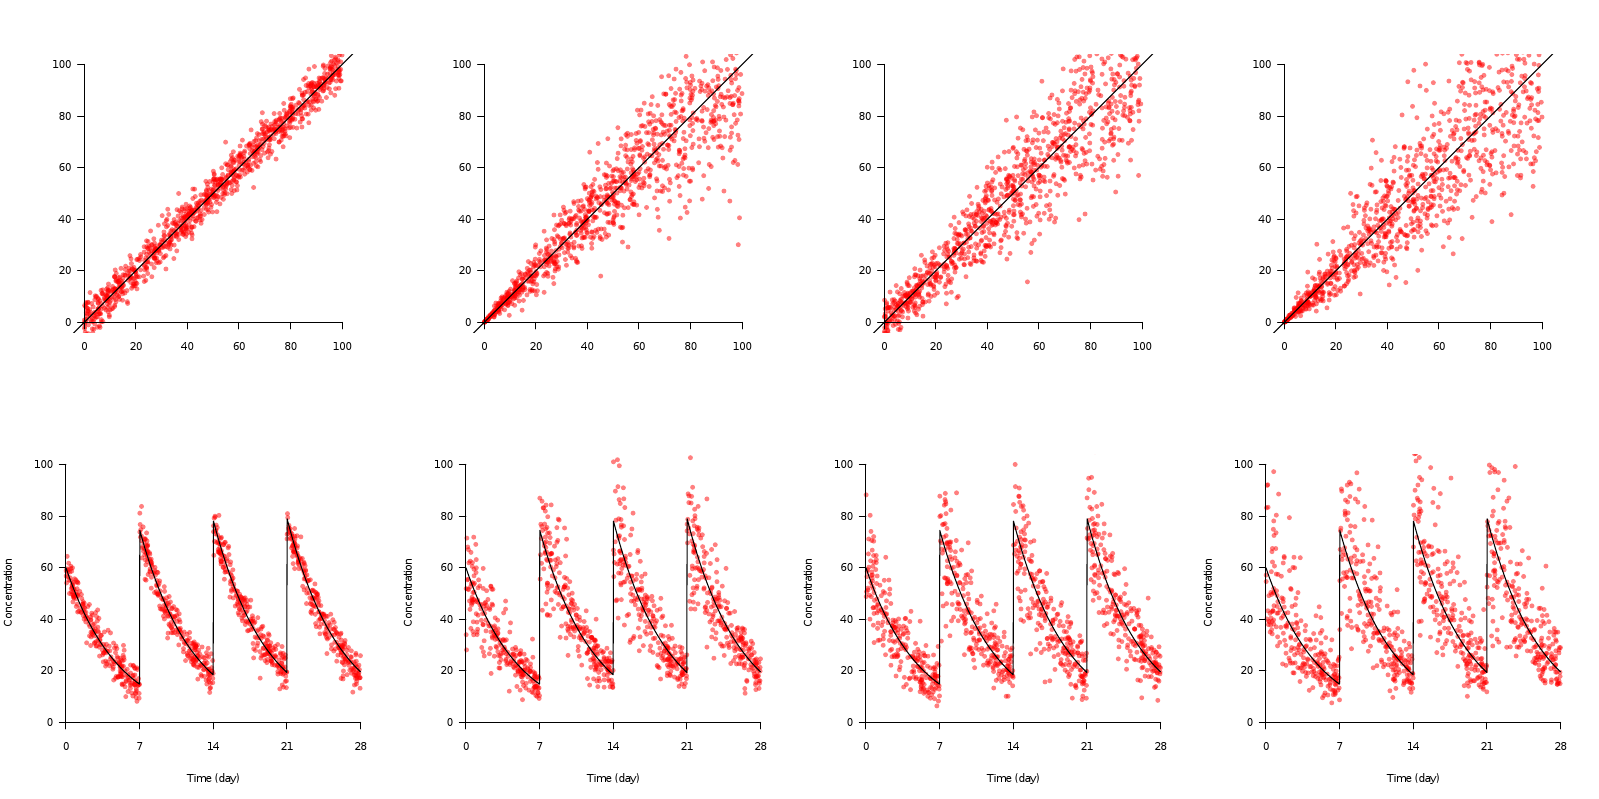
\includegraphics[width=10cm]{figures/raster/FIG_10}
	\caption[Visualisation de l'erreur résiduelle.]{Visualisation de l'erreur résiduelle. En haut, concentrations prédites vs. observées. En bas, concentrations observées au cours du temps avec la concentration prédite par les paramètres de population (ligne). De gauche à droite, modèle d'erreur additif, proportionnel, mixte, exponentiel.}
	\label{fig:10}
\end{figure}

\section{Les anticorps monoclonaux thérapeutiques}
\subsection{Généralités}
Les anticorps sont des glycoprotéines également appelées immunoglobulines (Ig) qui sont produits exclusivement par les lymphocytes B.

Les anticorps thérapeutiques peuvent être classés en trois grands groupes : les Ig polyvalentes, les Ig polyclonales et les anticorps monoclonaux. Les anticorps monoclonaux recombinants, utilisés en thérapeutique depuis les années 1980, ont révolutionné la prise en charge de nombreuses pathologies telles que le cancer, les maladies inflammatoires et certaines maladies immunologiques. En 1975, Kohler et Milstein ont réussi à fusionner une cellule lymphoïde normale et une cellule myélomateuse pour créer un hybridome, lignée cellulaire immortelle capable de produire un anticorps monoclonal de manière durable~\citep{REF13}. Ces anticorps monoclonaux sont tous identiques et reconnaissent le même épitope sur un antigène. Aujourd'hui, la production industrielle d'anticorps monoclonaux utilise des techniques d'expression d'ADN recombinant, le plus souvent dans des cellules de mammifères~\citep{REF14, REF15}. Les anticorps monoclonaux thérapeutiques commercialisés sont principalement des IgG1$\kappa$. Ils sont constitués de quatre chaînes polypeptidiques : deux chaînes lourdes d'isotype $\gamma$ ("H", de 50~k\gls{Da}) et deux chaînes légères d'isotype $\kappa$ ("L", de 25~k\gls{Da}), soit une masse moléculaire totale d'environ 150~k\gls{Da}. Chacune de ces chaînes possède des domaines variables ("V", correspondant à l'extrémité N terminale et se fixant sur l'antigène) et des domaines constants ("C ") . Les IgG sont constituées de deux portions Fab, contenant les parties variables, et d'une portion Fc (Figure~\ref{fig:11}a). La portion Fc a la capacité de fixer le complément (fraction C1q) et de recruter des cellules effectrices porteuses de récepteurs Fc$\gamma$R (Figure~\ref{fig:11}b)~\citep{REF16}.

\begin{figure}[htbp]
	\centering
		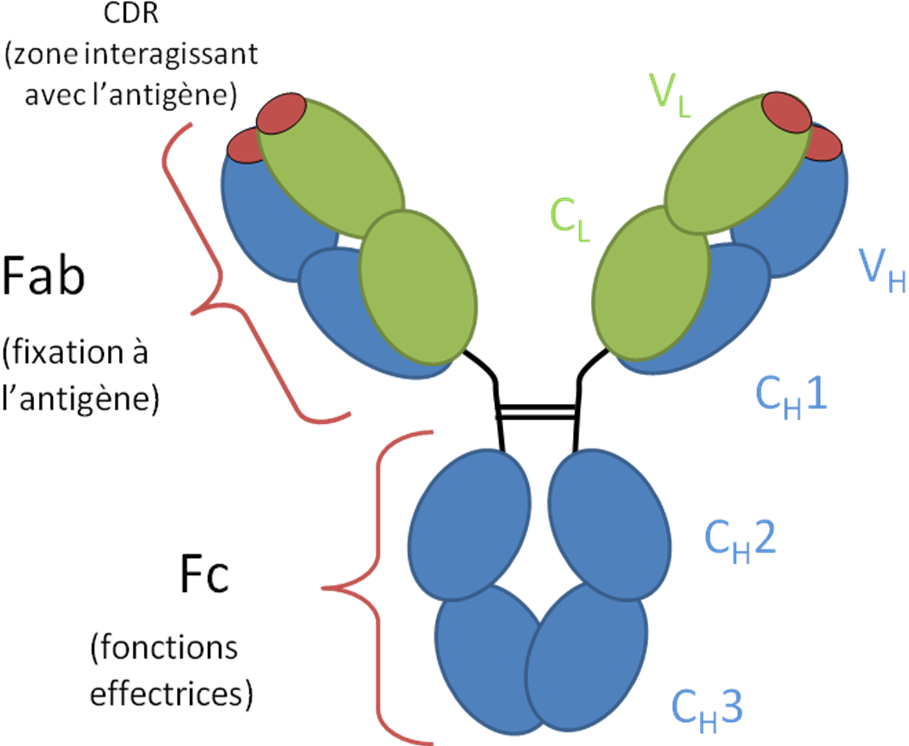
\includegraphics[width=5cm]{figures/raster/FIG_11a}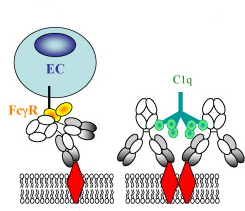
\includegraphics[width=5cm]{figures/raster/FIG_11b}
	\caption[Structure d'une IgG et rôle de la portion Fc.]{Structure d'une IgG et rôle de la portion Fc dans le mode d'action des anticorps se fixant sur un antigène membranaire. Grâce à leur portion Fc, les IgG1 peuvent recruter des cellules porteuses de récepteurs Fc$\gamma$R ou la fraction C1q du complément.}
	\label{fig:11}
\end{figure}

Les premiers anticorps monoclonaux produits étaient intégralement murins. Trois inconvénients ont limité leur utilisation en thérapeutique~\citep{REF17} :
\begin{itemize}
\item Une élimination trop rapide de l'organisme entraînant une faible efficacité.
\item Une faible capacité de la portion Fc murine de recruter les cellules effectrices humaines ou d'activer la voie classique du complément.
\item Une forte immunogénicité avec la production rapide d'anticorps anti-anticorps thérapeutique chez tous les patients traités.
\end{itemize}
Les progrès en biotechnologie ont permis de développer des anticorps chimériques, puis humanisés et enfin totalement humains, pour tenter de pallier ces inconvénients. Les anticorps chimériques comme le rituximab ou le cetuximab possèdent des régions variables murines et des régions constantes humaines. Pour les anticorps humanisés comme le bevacizumab ou le trastuzumab, seules les régions hypervariables sont d'origine animale. Enfin, les anticorps monoclonaux humains ne possèdent aucune région animale (Figure~\ref{fig:12}).

\begin{figure}[htbp]
	\centering
		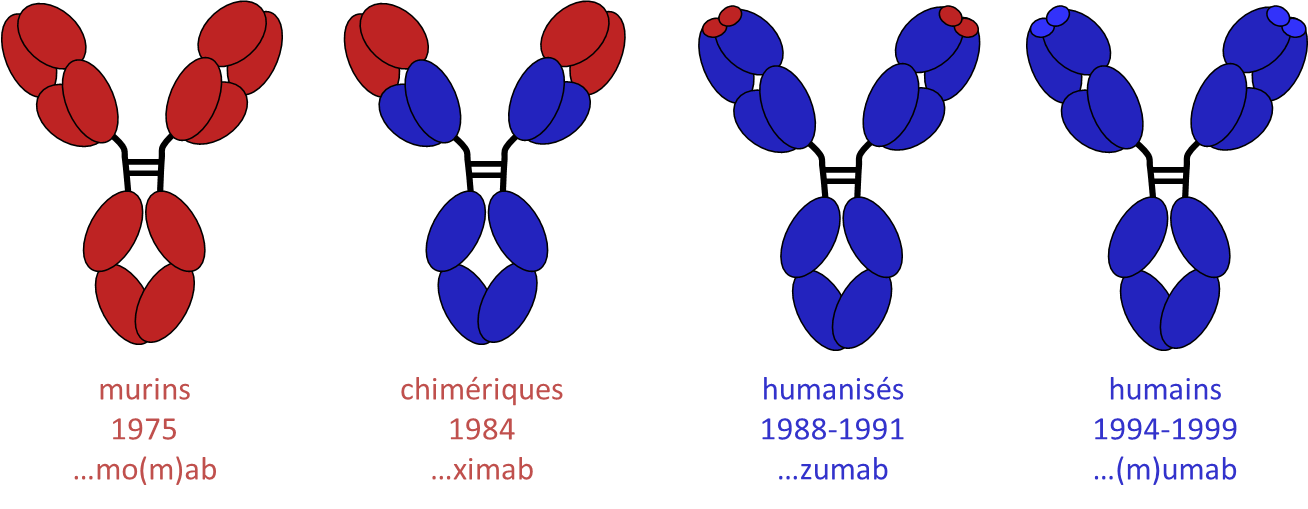
\includegraphics[width=10cm]{figures/raster/FIG_12}
	\caption[Différents degrés d'humanisation des anticorps thérapeutiques IgG.]{Différents degrés d'humanisation des anticorps thérapeutiques IgG. En rouge, les portions animales, en bleu, les portions humaines. $-o-$ : murin ; $-xi-$ : chimérique ; $-zu-$ : humanisé et $-u-$ : humain.}
	\label{fig:12}
\end{figure}

\subsection{Mécanismes impliqués dans la pharmacocinétique des anticorps monoclonaux}
Ne serait-ce que parce que ce sont des protéines de haute masse moléculaire (environ 150~k\gls{Da}), les anticorps monoclonaux ont des sources de variabilité pharmacocinétique différentes de celles des médicaments "classiques", molécules généralement issues d'une synthèse chimique et d'une masse moléculaire faible. Cependant, on peut décrire des phases d'absorption (pour les administrations par voie~\gls{EV}), de distribution et d'élimination.

\subsubsection{Absorption des anticorps monoclonaux}
La majorité des anticorps monoclonaux est administrée par voie~\gls{IV}, ce qui permet une exposition rapide et complète. Cependant, certains d'entre eux, comme l'adalimumab, un anti-TNF$\alpha$, sont administrés par voie sous cutanée (SC). L'administration~\gls{EV} représente un confort pour le patient puisque qu'elle est moins invasive et peut se faire à domicile. Cependant, l'absorption des anticorps monoclonaux est lente et donc difficile à quantifier précisément. Elle est par ailleurs incomplète. Nous verrons dans la discussion que ces voies d'administration sont une source de variabilité pharmacocinétique supplémentaire qu'il faut prendre en compte. Les mécanismes d'absorption des IgG après administration SC et~\gls{EV} en général n'ont jamais été directement étudiés~\citep{REF18}. 

\subsubsection{Élimination des anticorps monoclonaux}
Les anticorps sont principalement éliminés par deux mécanismes associés : un catabolisme non spécifique suivant leur endocytose passive et une élimination faisant suite à leur fixation sur l'antigène cible. Lorsqu'une immunisation survient les anticorps peuvent également être éliminés par la formation de complexes immuns.

\subsubsection{Captation par endocytose}
Comme l'ensemble des protéines circulantes, les anticorps pénètrent dans les cellules endothéliales vasculaires par endocytose passive~\citep{REF7, REF18}. Ce phénomène pourrait également se produire dans certains tissus (peau, muscles, foie et intestin)~\citep{REF19}. Mais un phénomène de protection contre la dégradation des IgG existe, dans lequel le FcRn joue un rôle clé.

\subsubsection{Rôle du FcRn dans l'élimination et de la distribution des anticorps monoclonaux}
La demi-vie ($t_{1/2}$) d'élimination de l'albumine et des IgG endogènes (à l'exception de celle des IgG3) est d'environ 21 jours chez l'homme, ce qui est plus long que celle des autres protéines et notamment des autres immunoglobulines (entre 2,5 et 6~jours)~\citep{REF20, REF21}. Par ailleurs, la demi-vie d'élimination du fragment Fc est du même ordre de grandeur que celle de l'IgG totale, alors que celle des fragments Fab est plus courte~\citep{REF22}. La portion Fc joue donc un rôle majeur dans la vitesse d'élimination des IgG.

A concentrations thérapeutiques, l'élimination des immunoglobulines polyvalentes administrées par voie intraveineuse est concentration-dépendante~\citep{REF23} mais à l'inverse des médicaments \og~classiques", leur $t_{1/2}$ d'élimination diminue lorsque leur concentration augmente~\citep{REF20} (Figure~\ref{fig:13}).

A partir de cette observation, Brambell, dans les années 1960, a émis l'hypothèse d'un récepteur spécifique et saturable protégeant les IgG du catabolisme endogène~\citep{REF24}. Ce récepteur est maintenant appelé FcRn (pour \textit{neonatal Fc receptor}) car il a été identifié pour la première fois dans l'épithélium intestinal de Rat nouveau-né~\citep{REF25}. Depuis, du FcRn a été trouvé chez d'autre rongeurs, chez le Singe, chez l'Homme~\citep{REF26} et il est maintenant admis qu'il est présent chez tous les mammifères. Chez l'Homme, FcRn a été identifié dans le poumon~\citep{REF27}, la barrière hémato-encéphalique, le foie~\citep{REF28}, les reins et d'autre organes~\citep{REF29}. C'est un homologue du complexe majeur d'histocompatibilité de classe~I qui est constitué de trois sous-unités : $\alpha$1, $\alpha$2 et $\alpha$3, et est associé de façon non covalente à la $\beta 2$-microglobuline. Chez la Souris~\citep{REF30, REF31} comme chez l'Homme~\citep{REF32, REF33}, le FcRn est responsable du transport materno-foetal des IgG à travers la barrière placentaire en fin de gestation.

\begin{figure}[htbp]
	\centering
		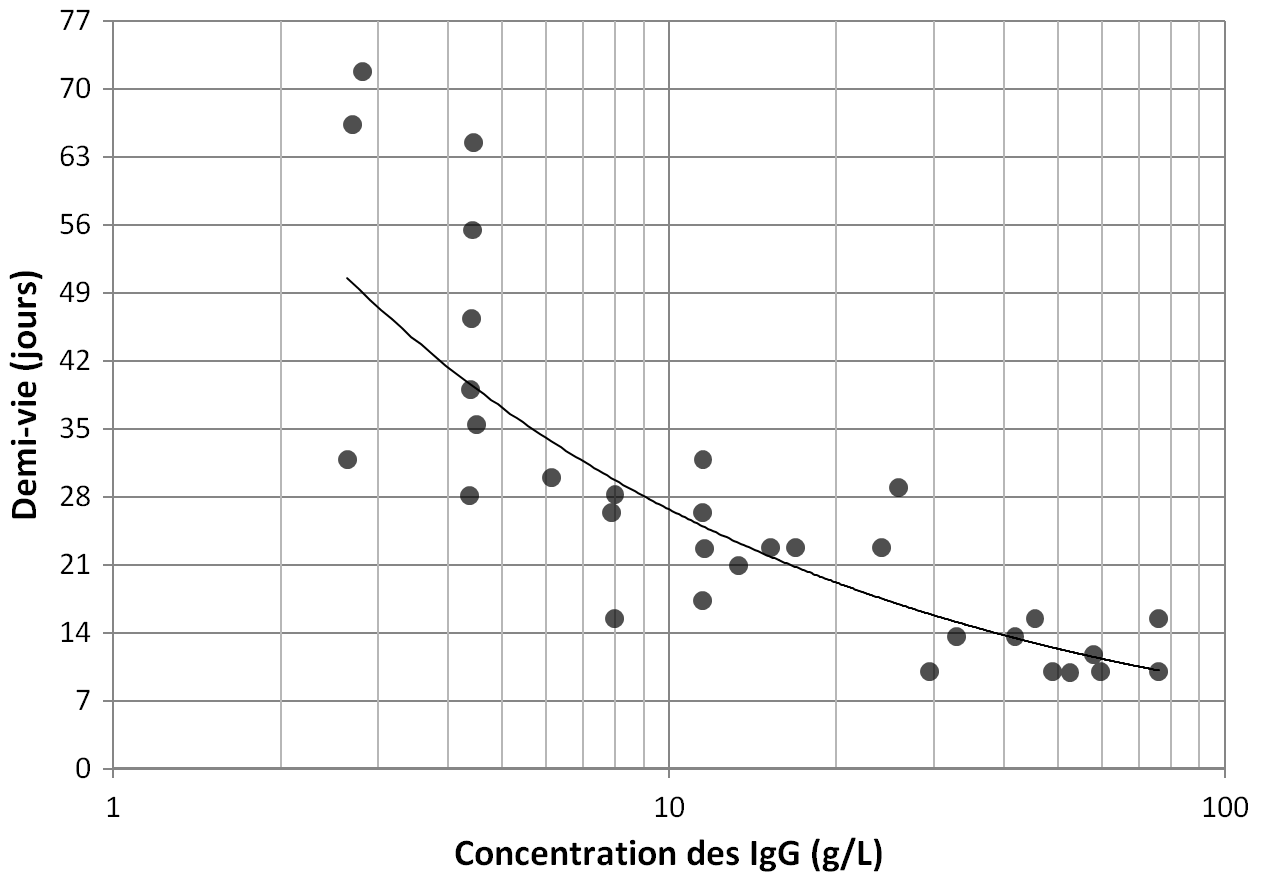
\includegraphics[width=10cm]{figures/raster/FIG_13}
	\caption[Relation entre la demi-vie des IgG et leurs concentrations sériques.]{Relation entre la demi-vie des IgG et leurs concentrations sériques. Adapté d'après Kuester K, Kloft C. Pharmacokinetics of monoclonal antibodies. In : Meibohm B, ed. Pharmacokinetics and pharmacodynamics of biotech drugs. Weinheim : Wiley-VCH Verlag, 2006.}
	\label{fig:13}
\end{figure}

L'interaction FcRn-IgG est pH dépendante : après leur endocytose passive (pinocytose) par les cellules endothéliales, les IgG se fixent à pH acide (6,0) au FcRn, à l'intérieur des vésicules d'endocytose. Cette dépendance au pH est en partie expliquée par la présence d'histidines dans les domaines CH$_2$ et CH$_3$ de la portion Fc~\citep{REF34, REF35}. Les protéines endocytées mais non fixées au FcRn sont dégradées dans les lysosomes~\citep{REF36, REF37}. La fixation au FcRn permet de détourner les IgG de la dégradation en permettant leur exocytose à pH neutre. On parle de recyclage ou de transcytose suivant si la vésicule est exocytée vers le pôle apical ou le pôle baso-latéral. (Figure~\ref{fig:14}). Plusieurs études ont confirmé le rôle décisif du FcRn dans l'homéostasie des IgG.

\begin{figure}[htbp]
	\centering
		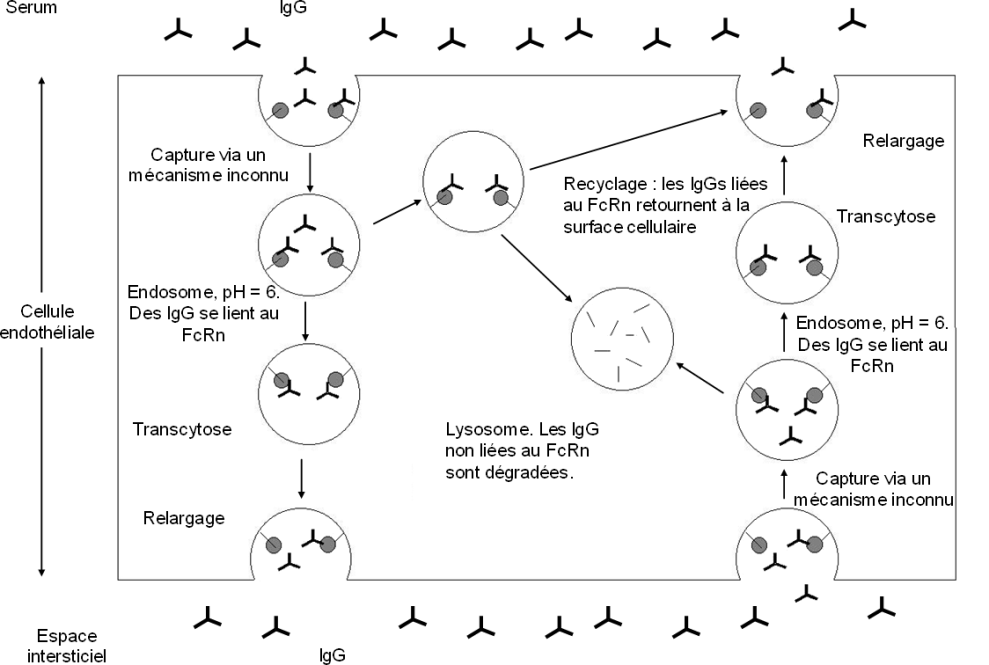
\includegraphics[width=10cm]{figures/raster/FIG_14}
	\caption[Rôle du FcRn]{Rôle du FcRn dans la protection des IgG de la dégradation et dans leur transport bidirectionnel à travers la cellule endothéliale. D'après Ghetie \& Ward, 1997.}
	\label{fig:14}
\end{figure}

L'albumine sérique est également recyclée par le FcRn mais sans phénomène de compétition avec le recyclage des IgG~\citep{REF38}.

Le FcRn d'une espèce animale donnée peut avoir une affinité pour les IgG d'une autre espèce. Ainsi, le FcRn de Souris est peu spécifique et fixe les IgG de plusieurs espèces (Lapin, Rat, Cochon d'Inde, Boeuf, Mouton et Homme), alors que le FcRn humain est plus sélectif et ne fixe que les IgG de Lapin et de Cochon d'Inde~\citep{REF36}. La courte $t_{1/2}$ d'élimination des IgG3 humaines par rapport aux IgG1, 2 et 4 peut être expliquée par leur faible affinité pour le FcRn~\citep{REF35}. Parmi les anticorps monoclonaux commercialisés, aucun n'est de type IgG3~\citep{REF39}.

Il n'existe pas de polymorphisme génétique rapporté sur les 5~exons de \textit{FCGRT}, le gène codant pour le FcRn. Cependant, les variations du nombre de répétitions en tandem (VNTR pour variable number of tandem repeats) dans l'intron~1 pourraient influencer la transcription~\citep{REF40}. Cette différence pourrait être une source de variabilité dans la vitesse de distribution et d'élimination des IgG.

Les IgG devraient théoriquement avoir une faible pénétration tissulaire en raison de leur masse moléculaire élevée et donc être confinés dans la circulation sanguine et les liquides extracellulaires \textbf{(Tang 2001)}. Cependant, une phase de distribution est clairement identifiable sur la courbe des concentrations en fonction du temps pour tous les IgG1. Le FcRn, en permettant la transcytose des IgG, joue vraisemblablement un rôle majeur dans leur distribution dans l'organisme~\citep{REF31, REF41}.

\subsubsection{Élimination après fixation sur la cible}
Le mécanisme d'action des anticorps thérapeutiques repose sur leur fixation sur un antigène-cible circulant ou membranaire. 

Dans le cas d'un antigène circulant, la formation puis l'élimination par le système immunitaire du complexe antigène-anticorps entraîne l'élimination de la cible et de l'anticorps. 

Dans le cas d'un antigène membranaire, la fixation de l'anticorps peut provoquer l'endocytose du complexe antigène-anticorps formé. Cette internalisation a par exemple été décrite après la fixation de l'efalizumab sur le CD11a (la sous-unité $\alpha$ du récepteur LFA-1). Après son internalisation, le complexe immun est retrouvé dans les lysosomes, puis est dégradé~\citep{REF42}. Une internalisation a également été décrite pour le complexe formé par le cetuximab et sa cible, l'EGFR~\citep{REF43}. La vitesse d'élimination par cette voie est le plus souvent limitée par la quantité de cible.

\subsubsection{Élimination liée à l'immunisation du sujet traité (immunogénicité)}
Théoriquement, le risque d'immunisation contre les anticorps décroît avec leur degré d'humanisation, c'est-à-dire : murins > chimériques > humanisés > totalement humains~\citep{REF44}. Cependant, les anticorps partiellement ou totalement humanisés peuvent également être immunogènes du fait de leur portion animale ou en raison d'une immunisation contre leur idiotype, qui peut toujours être reconnu comme du non-soi. Les anticorps induits sont responsables d'une accélération de l'élimination de l'anticorps thérapeutique et donc d'une diminution de son efficacité clinique et peuvent être à l'origine d'effets indésirables.

La structure des anticorps thérapeutiques n'est cependant pas le seul facteur influençant leur immunogénicité. En effet, le risque d'immunisation contre le rituximab, un anticorps chimérique anti-CD20, existe dans la polyarthrite rhumatoïde, alors qu'il semble inexistant chez les patients traités pour lymphome.
\subsection{Modélisation pharmacocinétique des anticorps monoclonaux}
Comme pour les médicaments "classiques", la pharmacocinétique des anticorps monoclonaux est principalement étudiée lors des phases initiales de leur développement clinique (phases~I et II) pour déterminer les doses qui seront testées en phase~III. Cependant, pour de nombreux anticorps monoclonaux actuellement sur le marché, la relation entre la concentration et l'effet in vivo est mal connue et/ou peu décrite dans la littérature et les données pharmacocinétiques sont insuffisamment utilisées lors du choix des doses à administrer. Une meilleure connaissance de la pharmacocinétique est donc une étape indispensable pour l'optimisation de l'utilisation thérapeutique des anticorps monoclonaux. Ce besoin d'amélioration du schéma posologique est particulièrement net en cancérologie. Il y a au moins deux raisons à cela : d'une part, au moment de la mise sur le marché, la connaissance de l'anticorps monoclonal est souvent incomplète car son développement clinique a été accéléré compte tenu de la gravité de la pathologie. D'autre part, une influence de la masse tumorale sur la pharmacocinétique des anticorps monoclonaux est suspectée~\citep{REF45, REF46, REF47}. Si cette influence est confirmée, ce facteur devrait être pris en compte pour améliorer l'adaptation posologique individuelle. De plus, l'analyse de la pharmacocinétique clinique des anticorps thérapeutiques est une étape nécessaire à l'étude de leur relation concentration-effet, outil indispensable à la fois pour un choix raisonné de la posologie et pour la compréhension de leur mécanisme d'action chez l'Homme. 

La pharmacocinétique n'a pas été étudiée avec le même niveau de détail pour tous les anticorps thérapeutiques. La pharmacocinétique de l'efalizumab (anti-CD11a) a été bien décrite~\citep{REF48, REF49, REF50}. La pharmacocinétique du rituximab a été assez bien étudiée~\citep{REF51, REF52}, mais la connaissance de la pharmacocinétique d'anticorps comme l'adalimumab et le bevacizumab, utilisés pourtant depuis plusieurs années, reste insuffisante. Les études de la pharmacocinétique des anticorps monoclonaux chez l'Homme ont utilisé l'approche non-compartimentale~\citep{REF53,REF54, REF55, REF56, REF57, REF58, REF59} et l'approche compartimentale. Dans ce cas, les modèles étaient parfois mono-compartimentaux~\citep{REF60} mais le plus souvent, bi-compartimentaux (tableau~\ref{tab:2}). Après administration~\gls{IV}, les concentrations d'anticorps monoclonaux décroissent en effet généralement de façon bi-exponentielle. Les anticorps se distribuent donc dans deux types de tissus, respectivement modélisés par un volume central de distribution $V_1$ et un volume périphérique $V_2$ avec une clairance de distribution $Q$ et une clairance d'élimination \gls{CL}. 

La description compartimentale de la pharmacocinétique des anticorps administrés par voie~\gls{EV} peut être réalisée en intégrant un compartiment d'absorption et une constante d'absorption $k_{a}$ d'ordre~1. Hayashi~\textit{et al.} ont par exemple décrit l'absorption de l'omalizumab (anti IgE) administré par voie sous cutanée (SC) à l'aide de ce modèle~\citep{REF61}. aucune modélisation de l'absorption d'un anticorps monoclonal reposant sur des compartiments de transit n'a pour l'instant été publiée. Compte tenu de la lenteur de l'absorption, la distribution de l'anticorps dans le compartiment périphérique est rarement identifiable ; pour cette raison, un modèle mono-compartimental est souvent utilisé.

\subsubsection{Dose-dépendance et élimination non-linéaire}
Des phénomènes d'éliminations saturables ont été décrits pour près de la moitié des anticorps monoclonaux commercialisés~\citep{REF62}. Leur clairance étant en partie due à leur fixation sur l'antigène-cible, un modèle mécanistique de type TMDD peut être utilisé si les données sont suffisamment riches. Les données disponibles étant rarement très riches, la description de ces phénomènes d'élimination saturable est souvent réalisée par une équation de type Michaelis-Menten~\citep{REF3}. Mould~\textit{et al.} ont par exemple décrit l'élimination de l'alemtuzumab par une équation de type Michaelis-Menten reliée au compartiment central. Kloft~\textit{et al.} ont décrit l'élimination du sibrotuzumab par une équation combinant clairance (élimination non saturable) et élimination de type Michaelis-Menten à partir du compartiment central~\citep{REF63}. Sharma~\textit{et al.} ont quant à eux décrit la pharmacocinétique du keliximab et du clenoliximab (deux anticorps anti CD4)  par un modèle à deux compartiments avec élimination de type Michaelis-Menten appliquée aux deux compartiments~\citep{REF64}.

Lorsque l'élimination n'est pas saturée, l'\gls{AUC} -- qui est le reflet de l'exposition -- est proportionnelle à la dose (équation~\ref{eq:1}). Dans ce cas, si l'intervalle d'injection $\tau$ est doublé, la même \gls{AUC} peut être obtenue en doublant la dose. Lorsque l'élimination fait intervenir des phénomènes saturables, cette relation n'est plus vraie et il est nécessaire de disposer d'un modèle compartimental intégrant ces phénomènes pour adapter la posologie selon l'objectif d'exposition.

Bien que les modèles de type TMDD soient théoriquement les mieux adaptés à la description mécanistique de l'élimination des anticorps monoclonaux, aucune publication n'a encore rapporté leur utilisation. Les caractéristiques non-linéaires de l'élimination sont généralement décrites par équation de Michaelis-Menten.  

\begin{table}[!ht]
  \centering
  \caption{Exemples de modèles de population utilisés pour décrire la pharmacocinétique des anticorps monoclonaux thérapeutiques.}
    \begin{tabular}{p{1.6cm}ccp{1.8cm}p{.8cm}p{.9cm}ccp{.9cm}l}
      &&&&&&&&& \\
      \hline
\textbf{Étude} & \textbf{Anticorps} & \textbf{Cible} & \textbf{Pathologie} & \textbf{Voie} & \textbf{Sujets (n)} & \textbf{Comp.} & \textbf{F} & \textbf{Élim.} & \textbf{Covariables} \\
      \hline
      \hline
      Mager 2003~\citep{REF65} & Abciximab & GpIIb/IIIa & Angioplastie coronaire & \gls{IV} perf & 47 & 2 & - & 1 & - \\
      Weisman 2003~\citep{REF66} & Adalimumab & TNF$\alpha$ & PR & \gls{IV} perf & 9 & 2 & - & 1 & \gls{CL} : sexe \\
      Mould 2007~\citep{REF67} & Alemtuzumab & CD52 & Leucémie lymphoïde chronique & \gls{IV} perf & 67 & 2 & - & MM & - \\
      Dirks 2008~\citep{REF68} & Cetuximab & EGFR & Cancer de la tête et du cou & \gls{IV} perf & 143 & 2 & - & MM & - \\
      Mould 2007~\citep{REF69} & Clenoliximab & CD4 & PR & \gls{IV} perf & 32 & 2 & - & MM & - \\
      Ng 2005~\citep{REF50} & Efalizumab & CD11a & Psoriasis modéré et sévère & SC & 240 & 2 & 56\% & 1+MM & - \\
      Dartois 2007~\citep{REF70} & Ilonimomab & CD25 & Maladie du greffon contre l'hôte & \gls{IV} perf & 21 & 2 & - & 1 & - \\
      Ternant 2008~\citep{REF71} & Infliximab & TNF$\alpha$ & maladies inflammatoires de l'intestin & \gls{IV} perf & 33 & 2 & - & 1 & V1 : Poids et sexe immunisation sur \gls{CL} \\
      Kuester 2009~\citep{REF72} & Matuzumab & EGFR & Cancer colorectal & \gls{IV} perf & 90+81 & 2 & - & 1+MM & \gls{CL} : Poids sec \\
      Hayashi 2007~\citep{REF61} & Omalizumab & IgE & Syndromes atopiques & SC & 910 & 1 & 62\% & 1 & $V_1/F$ : Poids,  âge et sexe \\
      Ma 2008~\citep{REF73} & Panitumumab & EGFR & Cancer colorectal & \gls{IV} perf & 1200 & 2 & - & 1+MM & Poids sur $V_1$, \gls{CL} et $V_{max}$ \\
      Iacona 2000~\citep{REF51} & Rituximab & CD20 & Lymphome NHF & \gls{IV} perf & 7 & 2 & - & 1 & - \\
      Ng 2005~\citep{REF52} & Rituximab & CD20 & PR & \gls{IV} perf & 102 & 2 & - & 1 & BSA et sexe sur $V_1$ et \gls{CL} \\
      Kloft 2004~\citep{REF74} & Sibrotuzumab & FAP & Cancers colorectal et du poumon & \gls{IV} perf & 60 & 2 & - & 1+MM & Poids sur $V_1$,  \gls{CL} et $V_{max}$ \\
      Frey 2010~\citep{REF75} & Tocilizumab & IL6R & PR & \gls{IV} perf & 1793 & 2 & - & 1+MM & - \\
      Bruno 2005~\citep{REF76} & Trastuzumab & HER2 & Cancer du sein métastatique & \gls{IV} perf & 476 & 2 & - & 1 & $V_1$ : Poids, ECD ; \gls{CL} : ECD, MET \\
      Zhu 2009~\citep{REF77} & Ustekinumab & IL12/23 & Psoriasis sévère & SC & 1937 & 1 & ? & 1 & Poids, diabète et immunisation sur $V_1/F$ et $\gls{CL}/F$ \\
      \hline
    \end{tabular}
  \label{tab:2}
\end{table}

\subsubsection{Facteurs de variabilité interindividuelle de la pharmacocinétique des anticorps monoclonaux.}
Comme nous l'avons évoqué plus haut, la plupart des études initiales~\citep{REF53, REF54, REF58, REF60}, ont rapporté une grande variabilité interindividuelle des concentrations résiduelles (avant l'injection suivante) pour une même dose. Cette grande variabilité a été confirmée par toutes les études pharmacocinétiques (Tableau 2), celles-ci ayant rapporté des CV interindividuels des paramètres compris entre 20\% et 50\%. Avec la généralisation de l'analyse pharmacocinétique de population, quelques facteurs de variabilité ont pu être identifiés, mais la majeure partie de cette variabilité demeure inexpliquée.
\paragraph{Facteurs démographiques et biochimiques.} Les facteurs démographiques (âge, poids, sexe, origine ethnique, surface corporelle, etc.) ainsi que certaines mesures biologiques (albuminémie, numérations sanguines, marqueurs de l'inflammation, etc.) sont montré une relation avec les paramètres pharmacocinétiques d'un anticorps thérapeutique. Le poids ou la surface corporelle sont souvent les principales covariables explicatives de la variabilité interindividuelle des volumes de distribution, ceux-ci augmentant avec la valeur de ces covariables~\citep{REF52, REF61, REF74, REF76, REF78, REF79, REF80}. Le sexe peut également influencer la pharmacocinétique des anticorps. Ternant~\textit{et al.} ont montré une influence du sexe sur le volume de distribution de l'infliximab~\citep{REF71}. 
Comme décrit plus haut, la distribution et l'élimination de l'albumine et des IgG sont liées. Fasanmade~\textit{et al.} ont observé une relation entre la concentration sérique d'albumine et la pharmacocinétique de l'infliximab chez les patients traités pour rectocolite hémorragique~\citep{REF81}. La clairance de l'infliximab était d'autant plus faible que les patients avaient une concentration d'albumine élevée. Pour expliquer ces résultats, les auteurs ont fait l'hypothèse que des concentrations faibles d'albumine sont le reflet d'une expression plus faible de FcRn, responsable d'un recyclage plus faible et donc d'une élimination plus importante de l'infliximab et de l'albumine. Ils ont proposé d'utiliser la concentration sérique d'albumine comme indicateur prédictif de l'exposition des patients à l'infliximab.
\paragraph{Immunisation}
L'immunisation contre les anticorps thérapeutiques augmente leur clairance. Ternant~\textit{et al.} ont montré que la clairance de l'infliximab était 2,7 fois plus élevée chez les patients ayant des anticorps anti-infliximab (\gls{ATI} pour \textit{antibodies toward infliximab})~\citep{REF71} que chez les patients non immunisés.

\subsection{Facteurs de variabilité de la relation dose-concentration-effet des IgG}
Un des premiers facteurs individuels de variabilité de la réponse aux anticorps thérapeutiques identifié est un polymorphisme génétique du récepteur Fc$\gamma$RIIIA (CD16a) codé par le gène FCGR3A. Ce polymorphisme conduit à la présence d'une phénylalanine ou d'une valine en position~\citep{REF158}. En effet, la survie sans progression de patients traités par rituximab, un anti-CD20, pour lymphome malin non Hodgkinien était significativement plus longue chez les patients homozygotes de génotype FCGR3A-158V/V que chez les patients porteurs de l'allèle FCGR3A-158F~\citep{REF82}. Ce polymorphisme génétique influence l'affinité du récepteur Fc$\gamma$RIIIA pour la portion Fc des IgG et donc le recrutement des cellules impliquées dans la cytotoxicité à médiation cellulaire dépendante des anticorps (\gls{ADCC} pour \textit{Antibody-Dependent Cell-mediated Cytotoxicity})~\citep{REF83, REF84}. L'influence de ce polymorphisme sur l'efficacité du rituximab a été confirmée par d'autres études~\citep{REF85, REF86} et a également été mis en évidence pour d'autres anticorps thérapeutiques agissant au moins en partie par \gls{ADCC}, comme un anticorps anti-D~\citep{REF87}, l'infliximab~\citep{REF88} et le trastuzumab~\citep{REF89}.

Comme ce polymorphisme entraîne une différence d'affinité du récepteur Fc$\gamma$RIIIA pour la portion Fc des anticorps thérapeutiques, il était logique de penser qu'il n'influence pas la pharmacocinétique des anticorps mais plutôt leur relation concentration-effet. Ceci a été confirmé pour le rituximab par un modèle \textit{in vitro}~\citep{REF83}, puis chez l'Homme par la modélisation de la relation concentration-effet de la Lymphoglobuline~\citep{REF86}.

Comme pour les médicaments classiques, les autres sources potentielles de variabilité de la relation concentration-effet sont le type de maladie et les traitements associés~\citep{REF7}. 

\subsection{Méthodes de mesure des concentrations des anticorps monoclonaux}
Afin de pouvoir réaliser des études pharmacocinétiques, il faut disposer d'une technique analytique validée. La première étape de la validation est la sélection d'une méthode de dosage appropriée à l'analyte et à sa matrice. Dans le cadre des études de cette thèse, l'analyte est un anticorps monoclonal. Compte tenu de sa masse moléculaire très élevée, la mesure de sa concentration ne peut pas être réalisée avec les mêmes techniques que celles utilisées pour les médicaments "classiques". Par ailleurs, le sérum, matrice dans laquelle l'analyse est habituellement réalisée, contient de nombreuses protéines et notamment d'autres anticorps. La méthode de mesure doit donc permettre d'estimer des concentrations sériques d'anticorps monoclonaux pouvant être inférieures à 1 mg/L alors qu'ils sont mélangés avec des IgG1 endogènes ayant des concentrations de l'ordre de 9 g/L~\citep{REF90}. Plusieurs méthodes de dosage des anticorps monoclonaux sont décrites dans la littérature~\citep{REF91} :

\begin{description}
\item[Résonance plasmonique de surface (BiaCore\textsuperscript{\textregistered}) :] Cette technique consiste à envoyer un faisceau de lumière monochromatique polarisée sur une puce sur laquelle un antigène-cible a été fixé, puis à mesurer les variations de l'angle de réflexion du faisceau dues à la modification de masse liée à la fixation antigène–--anticorps. Cette méthode est très précise, mais trop lourde pour envisager son utilisation en routine~\citep{REF92}.
\item[Chromatographie :] Ces méthodes sont prometteuses, car elles sont très rapides. Cependant, le développement est encore limité en raison de la matrice (le sérum) qu'il faut préalablement immuno-purifier. Yang~\textit{et al.} ont développé une technique de dosage d'un anticorps thérapeutique (non spécifié) par LC-MS/MS~\citep{REF93}. Une autre méthode expérimentale de dosage du cetuximab par LC-MS/MS a également été publiée~\citep{REF94}.
\item[Bio-analyses :] Ces techniques permettent d'estimer les concentrations d'anticorps monoclonaux en mesurant leur activité biologique \textit{ex vivo}. La variabilité des cellules cibles utilisées peut cependant poser des problèmes de reproductibilité, ce qui rend cette approche inadaptée en recherche clinique ou en suivi thérapeutique.
\item[Immunoanalyses : ] Cet ensemble de techniques permet de quantifier les concentrations d'anticorps monoclonaux grâce à l'interaction antigène-anticorps. La méthode E.L.I.S.A. (ou ELISA pour \textit{Enzyme Linked ImmunoSorbent Assay})~\citep{REF95}, comme les méthodes précédemment citées, peut être utilisée sous plusieurs formes. Parmi les principales méthodes ELISA, on peut citer (\ref{fig:15}) :
\begin{itemize}
\item ELISA directe : La détection directe utilise un anticorps marqué ou couplé à une enzyme qui reconnait directement l'antigène fixé. Cette technique ne permet pas de quantifier l'anticorps mais est utilisée pour la coloration immuno-histochimique de tissus ou de cellules.
\item ELISA indirecte : La détection indirecte est la plus utilisée et principalement pour le dosage des anticorps monoclonaux~\citep{REF96}. Dans ce cas, l'antigène fixé est reconnu par l'anticorps primaire que l'on veut doser. Un anticorps secondaire marqué ou couplé à une enzyme va ensuite reconnaitre spécifiquement l'anticorps primaire.
\item ELISA sandwich : Cette technique permet le dosage d'un antigène. Dans ce cas, un anticorps de capture, reconnaissant l'antigène à doser est fixé au fond du puits. L'antigène se fixe sur l'anticorps, puis un anticorps secondaire marqué ou couplé à une enzyme, reconnait un autre épitope de l'antigène.
\end{itemize}
\end{description}

\begin{figure}[htbp]
	\centering
		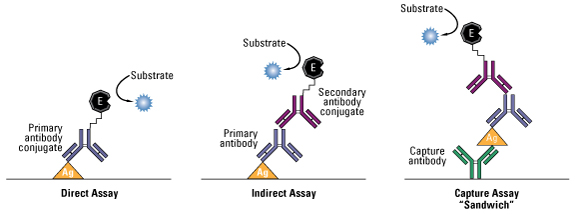
\includegraphics[width=10cm]{figures/raster/FIG_15}
	\caption{Principes des trois formes de technique ELISA.}
	\label{fig:15}
\end{figure}

Si elle n'est pas répétable et reproductible, la méthode de dosage peut également être une source d'imprécision et biaiser de façon importante l'analyse pharmacocinétique.

\section{Le cetuximab}

\subsection{Modes d'action du cetuximab}
Le cetuximab (Erbitux\textsuperscript{\textregistered}, Merck-Serono, Darmstadt, Allemagne) est un anticorps monoclonal recombinant de type IgG1$\kappa$. Il reconnaît spécifiquement le récepteur du facteur de croissance épidermique (EGFR pour \textit{Epidermal Growth Factor Receptor}), récepteur transmembranaire ayant une activité tyrosine kinase (TK). À l'état physiologique, l'EGFR est présent à la surface des cellules majoritairement dans une conformation compactée. Une petite fraction d'entre eux se trouve sous forme relâchée, permettant la fixation des ligands comme l'EGF ou le TGF$\alpha$ sur les domaines~I et III~\citep{REF97}. Cette fixation permet alors de démasquer le domaine II qui interagit avec le domaine~II d'un autre récepteur de la superfamille des EGFR (Figure~\ref{fig:16}).

\begin{figure}[htbp]
	\centering
		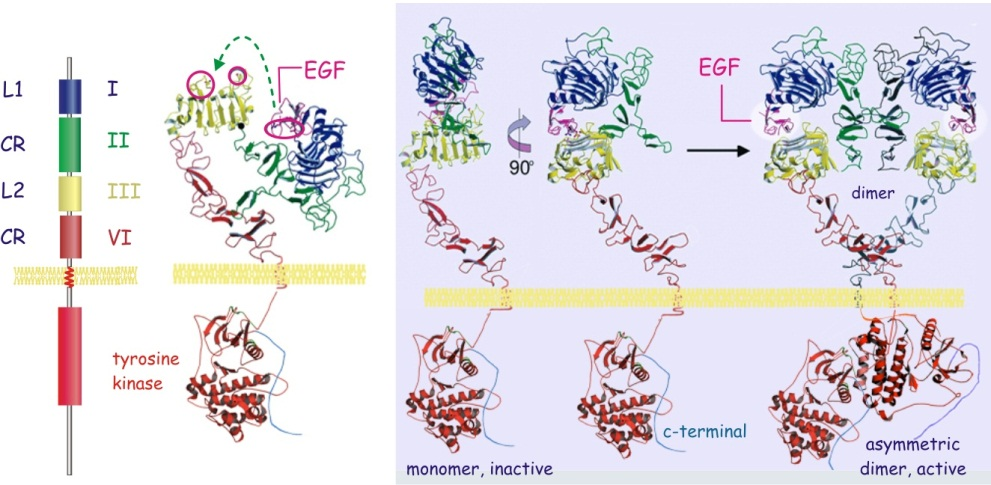
\includegraphics[width=10cm]{figures/raster/FIG_16}
	\caption[Structure de l'EGFR]{L'EGFR est constitué de trois domaines : un domaine intracellulaire qui possède une activité tyrosine kinase, un domaine transmembranaire et un domaine extracellulaire subdivisé en quatre sous-domaines (I, II, III et~IV). La fixation du ligand sur les sous-domaines~I et III permet de démasquer le domaine~II et donc la dimérisation avec un autre récepteur.}
	\label{fig:16}
\end{figure}

La dimérisation des récepteurs entraîne l'activation des domaines tyrosine kinase intracellulaires. Plusieurs voies de transduction du signal sont alors activées~\citep{REF98}. La voie Ras/Raf-MAPK aboutit à l'activation de facteurs de transcription via ERK, à l'origine de la prolifération cellulaire~\citep{REF99}. L'EGFR phosphorylé peut également activer la PI3 kinase (PI3K), qui mène à un signal anti-apoptotique~\citep{REF100}. L'EGFR possède également un rôle dans la prolifération et la survie cellulaire via JAK2/STAT3~\citep{REF101}. D'autres voies de signalisation sont impliquées dans l'adhésion cellulaire et l'angiogenèse. EGFR est exprimé dans de nombreux tissus épidermiques sains, comme la peau ou les follicules pileux, et est surexprimé ou stimulé de manière excessive dans certains cancers~\citep{REF102}.
Le cetuximab se fixe sur le domaine~III de l'EGFR, empêchant ainsi le démasquage du domaine~II et donc la dimérisation des récepteurs. De nombreuses études in vitro ont montré que le cetuximab inhibe ainsi des phénomènes d'angiogenèse et de prolifération cellulaire et qu'il entraîne une restauration de l'apoptose~\citep{REF103}. Une internalisation du complexe cetuximab-EGFR a également été décrite~\citep{REF43}. D'autres études in vitro sur cellules surexprimant EGFR ont montré que le cetuximab peut également à forte concentration entraîner la phosphorylation de l'EGFR et donc induire une transduction de signal \textbf{(Mandic, Rodgarkia-Dara~\textit{et al.} 2006; Yoshida, Okamoto~\textit{et al.} 2008)}. Cet effet de type agoniste vis-à-vis de l'EGFR est donc susceptible d'être observé \textit{in vivo} pour des concentrations élevées de cetuximab.

\subsection{Indications et posologie du cetuximab}
Le cetuximab est actuellement indiqué dans le traitement des patients ayant un cancer colorectal métastatique exprimant l'EGFR avec gène KRAS de type sauvage (\textit{wild-type}), en association avec une chimiothérapie, ou en monothérapie après échec d'un traitement à base d'oxaliplatine (FOLFOX) ou d'irinotecan (FOLFIRI) ou en cas d'intolérance à l'irinotecan~\citep{REF104}.

Le cetuximab est également indiqué dans le traitement des patients ayant un carcinome épidermoïde de la tête et du cou, en association avec la radiothérapie en cas de maladie localement avancée~\citep{REF105}, ou en association avec la chimiothérapie à base de platine en cas de maladie récidivante et/ou métastatique~\citep{REF106}.

Dans ces deux indications, le cetuximab est injecté par voie intraveineuse (\gls{IV}) toutes les semaines. La dose de charge recommandée est de 400 mg/m$^2$ pour la première perfusion qui se déroule sur deux heures. La dose de maintenance hebdomadaire est de 250 mg/m$^2$.

Les conditions de prescription dans le cancer colorectal ont évolué au cours du temps. En effet, la surexpression d'EGFR n'est plus un critère strict d'inclusion puisque des études ont montré que le nombre de copies d'EGFR n'influence pas significativement le bénéfice clinique 107-109. De plus, la mutation tumorale de KRAS n'était pas un critère d'exclusion au moment de l'autorisation de mise sur le marché (\gls{AMM}) du cetuximab en juin 2004. Depuis, plusieurs études ont montré que la réponse au cetuximab est restreinte aux patients porteurs de tumeurs avec KRAS non muté~\citep{REF110, REF111, REF112, REF113}.

Une méta-analyse a récemment montré que la survie sans progression des patients dont la tumeur avait la mutation KRAS G13D était meilleure que celle des patients ayant une tumeur avec une autre mutation~\citep{REF114}. Une autre étude a montré que le statut KRAS peut varier entre la tumeur primaire et les métastases chez un même patient~\citep{REF115}. D'autres polymorphismes génétiques tels que PTEN ou BRAF pourraient également avoir une influence sur l'efficacité du cetuximab~\citep{REF116, REF117}.

Dans le cancer colorectal métastatique, la chimiothérapie associée est administrée toutes les deux semaines alors que la posologie de l'\gls{AMM} du cetuximab est d'une injection hebdomadaire. Pour éviter au patient d'être hospitalisé toutes les semaines, l'injection d'une double dose (500 mg/m$^2$) de cetuximab toutes les deux semaines est couramment pratiquée. Cependant, les données publiées à ce jour~\citep{REF118} n'ont pas permis de démontrer clairement l'équivalence de cette posologie avec celle de l'\gls{AMM}. 

D'autres indications du cetuximab comme le cancer cutané~\citep{REF119} sont également activement explorées. Plusieurs essais de phase~II et de phase~III ont évalué l'intérêt du cetuximab en association à une chimiothérapie à base de sels de platine en 1ère ligne de traitement de cancers bronchiques non à petites cellules, avancés ou métastatiques~\citep{REF120, REF121}. Les résultats de ces essais montrent un bénéfice modeste en termes de survie globale (OS pour \textit{Overall Survival}) et de survie sans progression (PFS pour \textit{Progression-Free Survival}), associé à une toxicité non négligeable. Ces données ne montrant pas de rapport bénéfice/risque suffisant, le cetuximab n'a pas encore obtenu d'\gls{AMM} dans cette indication.

\subsection{Méthodes de mesure des concentrations de cetuximab}
Deux types de techniques de dosage ont été rapportées pour mesurer les concentrations sanguines de cetuximab chez l'Homme ou l'animal : les méthodes ELISA~\citep{REF122, REF123, REF124} et la résonnance plasmonique de surface (BiaCore)~\citep{REF125}. Les limites basses de quantification des méthodes ELISA étaient de l'ordre de 0,1 mg/L mais les étapes de validation n'ont pas été décrites.

\subsection{Pharmacocinétique des anticorps anti-EGFR}
La pharmacocinétique du cetuximab a été peu décrite. Les analyses qui ont été réalisées sont principalement non-compartimentales~\citep{REF118, REF122, REF126}. Cependant, comme pour la plupart des anticorps thérapeutiques, l'élimination du cetuximab est en partie concentration-dépendante en raison de la quantité limitée de cibles (EGFR)~\citep{REF123, REF127, REF128}. La vitesse d'élimination varie donc avec la concentration (et donc en fonction du temps), ce qui invalide l'approche non-compartimentale si les données sont pauvres. En revanche, l'approche compartimentale peut permettre de quantifier de manière plus précise des phénomènes d'élimination saturables.

Dirks~\textit{et al.} ont décrit la pharmacocinétique du cetuximab chez des patients traités pour carcinome épidermoïde de la tête et du cou par approche compartimentale de population. L'élimination y était quantifiée grâce à une équation de type Michaelis-Menten (équation~\ref{eq:34})~\citep{REF68}. Dans cette étude, le poids idéal et la numération leucocytaire étaient des covariables influençant significativement $V_{max}$, tandis que le poids influençait significativement $V_1$. Chez les patients traités pour cancer colorectal métastatique, il n'existe pas de publication décrivant une analyse compartimentale du cetuximab. Les facteurs influençant la variabilité de sa pharmacocinétique dans cette pathologie n'ont donc pas été étudiés.

Le matuzumab est une autre IgG anti-EGFR dont le développement a été arrêté en février 2008 par manque d'efficacité. Sa pharmacocinétique a cependant été décrite par approche compartimentale, à l'aide d'un modèle à deux compartiments avec élimination linéaire (\gls{CL}) couplée à une élimination saturable de type Michaelis-Menten~\citep{REF72, REF129}. La masse maigre était une covariable influençant significativement \gls{CL}. La pharmacocinétique du panitumumab (IgG2 anti-EGFR) a également été décrite par ce modèle~\citep{REF73}. Le poids était la covariable la plus influente, reliée à \gls{CL}, $V_{max}$, et $V_1$.

\subsection{Relations dose-réponse et concentration-réponse du cetuximab}
Peu de descriptions de la variabilité de la relation dose-réponse ou concentration-réponse ont été publiées.

Dans une étude portant sur 35 patients traités par cetuximab pour un cancer colorectal métastatique, Zhang~\textit{et al.} ont quantifié le risque relatif de progression des patients homozygotes \textit{FCGR2A}-131R/R ou \textit{FCGR3A}-158V/V comme étant $2,51$ fois supérieur à celui des patients porteurs des allèles \textit{FCGR2A}-158H et \textit{FCGR3A}-158F ($p = 0,004$)~\citep{REF130} Cependant, ce sont les allèles \textit{FCGR2A}-131H et \textit{FCGR3A}-158V qui sont associées à une meilleure affinité pour la portion Fc des IgG. Dans l'analyse de survie sans progression de Zhang~\textit{et al.}, la comparaison du groupe "\textit{FCGR2A}-131R/R ou \textit{FCGR3A}-158V/V" avec le groupe "\textit{FCGR2A}-158H et \textit{FCGR3A}-158F" n'est donc pas pertinente et invalide les résultats. Bibeau~\textit{et al.} ont étudié l'influence des polymorphismes de \textit{KRAS}, \textit{FCGR2A} et \textit{FCGR3A} sur la relation dose-réponse~\citep{REF131}. L'étude de 69 patients porteurs de cancer colorectal métastatique traités par cetuximab et irinotecan a montré une meilleure PFS chez les patients porteurs de tumeurs non mutées KRAS (5,3 mois vs 3,0 mois ; p = 0,021). Les patients ayant le génotype Fc$\gamma$RIIA-131H/H et/ou Fc$\gamma$RIIIA-158V/V avaient une meilleure PFS que les autres patients (5,5 vs 3,0 ; p = 0,005).

Des études ont décrit une relation entre la toxicité cutanée du cetuximab et son efficacité~\citep{REF132} et entre la concentration de cetuximab et la toxicité cutanée~\citep{REF122}. Dans cette dernière étude, qui est la seule publiée décrivant la relation concentration-effet du cetuximab \textit{in vivo}, Fracasso~\textit{et al.} ont monté dans une cohorte de 39 patients traités par cetuximab pour différents types de carcinomes, que les patients répondeurs avaient un grade de première toxicité cutanée plus important que les autres patients. Fracasso~\textit{et al.} ont également observé que les patients stables et les patients répondeurs avaient une concentration résiduelle moyenne plus élevée que les patients en progression : 60 mg/L vs 30 mg/L~\citep{REF122}.
 
%%%%%%%%%%%%%%%%%%%%%%%%%%%%%%%%%%%%%%%%%%%%%%%%%%%%%%%%%%%%%%%%%%%%%
%Les objectifs :
\chapter{Objectifs}
%\addcontentsline{toc}{chapter}{Objectifs}
%\markright{\MakeUppercase{Objectifs}}

L'objectif de notre travail était d'étudier la pharmacocinétique du cetuximab afin d'identifier ses sources de variabilité interindividuelles, d'étudier son influence sur la réponse clinique et d'explorer de nouveaux modes d'administration. Pour répondre à cet objectif, les travaux suivants ont été réalisés :


\begin{itemize}
\item Étude de la pharmacocinétique du cetuximab durant la dialyse rénale (publication~I). Le dysfonctionnement d'organes peut entraîner une modification de la pharmacocinétique des médicaments conventionnels. Peu de données sont disponibles sur la pharmacocinétique des anticorps monoclonaux chez les patients avec insuffisance rénale terminale traités par dialyse.


\item Étude des facteurs influençant la pharmacocinétique du cetuximab dans le cancer colorectal métastatique (Publications~II~et~III). Bien qu'il soit indiqué dans le traitement du cancer colorectal métastatique, la pharmacocinétique du cetuximab n'avait jamais été étudiée de façon précise dans cette pathologie. Notre étude a eu pour but de décrire la relation entre la dose et la concentration de cetuximab au cours du temps, dans le cancer colorectal métastatique par approche de population afin d'identifier ses sources de variabilité.


\item Étude de l'influence de la pharmacocinétique sur la réponse au cetuximab dans le cancer colorectal métastatique (publication~III). Grâce à l'étude décrite ci-dessus, nous avons étudié la relation entre la pharmacocinétique du cetuximab et la survie sans progression.


\item Étude de l'espacement des perfusions sur l'exposition des patients (manuscrit~IV). Grâce au modèle de l'étude~IV, nous avons simulé les concentrations obtenues avec différentes doses de cetuximab administrées toutes les une, deux ou trois semaines.


\item Étude de l'exposition au cetuximab après administration pulmonaire (publication~V). La nébulisation est une voie d'administration~\gls{EV} prometteuse pour le traitement du cancer broncho-pulmonaire. Nous avons étudié la biodisponibilité du cetuximab administré par nébulisation chez la Souris, étape indispensable avant une éventuelle étude clinique.
\end{itemize}

 
%%%%%%%%%%%%%%%%%%%%%%%%%%%%%%%%%%%%%%%%%%%%%%%%%%%%%%%%%%%%%%%%%%%%%
%Matériel et Méthodes :
\chapter{Méthodes}

\section{Développement et validation de la méthode ELISA de dosage du cetuximab.}

\subsection{Principes de l'ELISA indirect}

Nous avons développé et validé une méthode de mesure des concentrations sériques de cetuximab par ELISA indirecte (Publication~II). Les différentes étapes de cette méthode schématisées sur la Figure 17 sont les suivantes :
\begin{itemize}
\item la sensibilisation des puits de la plaque (une ligne sur deux) avec de l'EGFR recombinant.
\item la saturation de tous les puits avec de l'albumine pour limiter les fixations non spécifiques.
\item le dépôt des échantillons éventuellement dilués dans du sérum. 
\item le dépôt du conjugué qui est une portion F(ab)'2 d'anticorps de Chèvre couplée à une peroxydase et qui reconnait spécifiquement la chaîne ? des IgG humaines. 
\item le dépôt du substrat, un mélange de peroxyde d'hydrogène (H$_2$O$_2$) et d'ortho-phénylène diamine (OPD).
\item La réaction chimique catalysée par la peroxydase qui donne de l'eau (H$_2$O) et du 
2-3~diaminophénazine (coloration jaune).
\item Arrêt de la réaction par de l'acide sulfurique (H$_2$SO$_4$) qui dénature les protéines.
\item Lecture de l'absorbance à 492 et 620~nm puis interprétation.
\end{itemize}

\begin{landscape}
\begin{figure}[htbp]
	\centering
		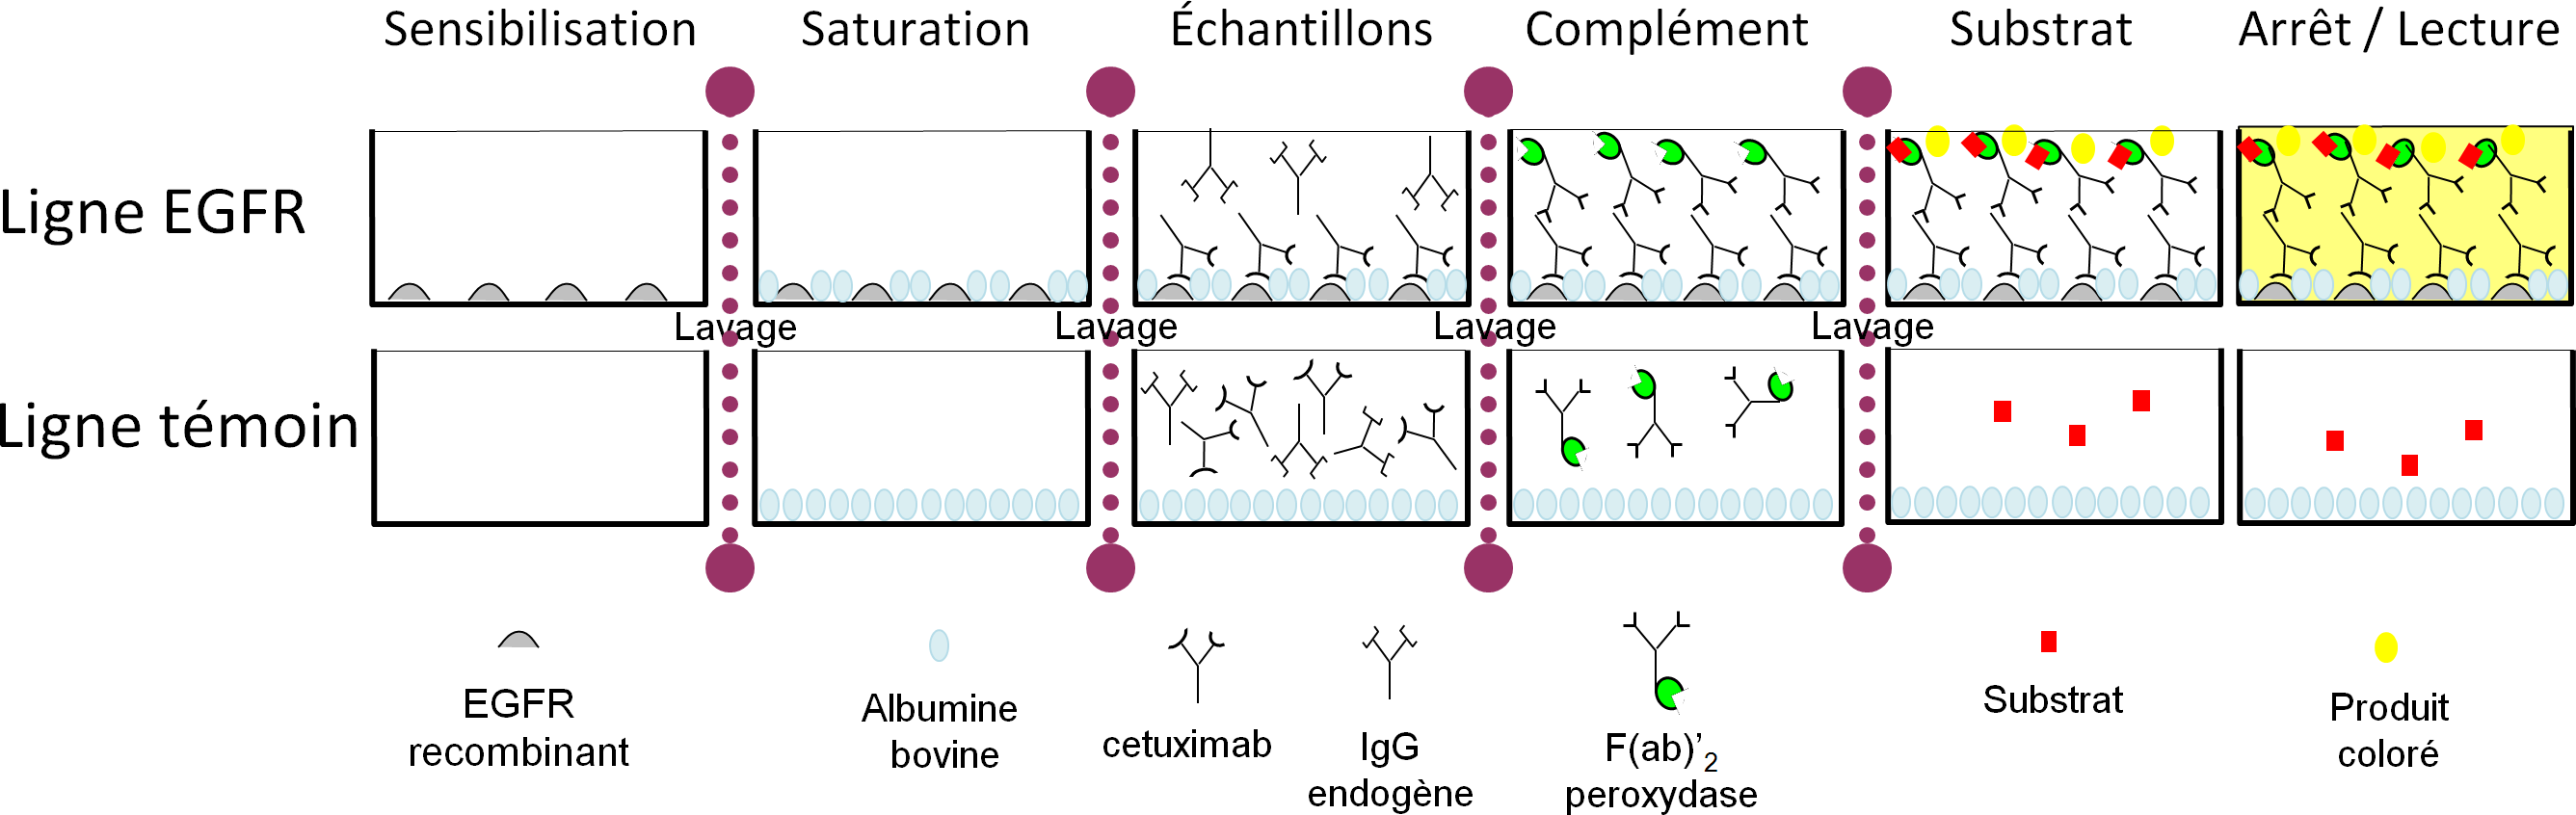
\includegraphics[width=20cm]{figures/raster/Figure17_ELISA}
	\caption[Étapes de la technique ELISA de dosage du cetuximab.]{Étapes de la technique ELISA de dosage du cetuximab. Chaque échantillon était déposé en double, dans un puits contenant de l'EGFR et dans un puits témoin sans EGFR. Pour chaque plaque, la mesure de 9 points de calibration et de 3 points de contrôle était réalisée. Avec une plaque de 96 puits, il était ainsi possible d'estimer la concentration de cetuximab de 12 échantillons de sérum.}
	\label{fig:17}
\end{figure}
\end{landscape}

\subsection{Développement}
Après avoir testé sans succès deux EGFR recombinants disponibles dans le commerce, nous avons produit notre propre EGFR recombinant. La mise au point et l'optimisation de cette production ont été réalisées par F. Piller (CNRS, Centre de Biophysique Moléculaire UPR~4301, Orléans, France). Des cellules HEK (cellules de rein de Hamster) ont été transfectées par un plasmide codant pour l'EGFR. Des modifications dans la séquence ont été apportées pour que la protéine soit sécrétée dans le surnageant et un \textit{tag} histidines a été ajouté pour permettre la purification sur billes de nickel. L'EGFR obtenu avait une concentration de l'ordre de 1~g/L.

A l'aide de sérums de 28 patients n'ayant jamais reçu de cetuximab, La limite de détection (LOD) était déterminée à 0,012~mg/L grâce à l'équation suivante :
\begin{equation}
54
\end{equation}
où  est la concentration moyenne estimée pour les sérums de patients n'ayant jamais reçu de cetuximab et  est l'écart-type. 

Les concentrations des points de calibration ont été réparties de façon régulière sur l'échelle logarithmique des concentrations entre 0 et 30~mg/L. La courbe de calibration était obtenue par régression logistique à l'aide de l'équation suivante :
\begin{equation}
55
\end{equation}
où $Abs$ était l'absorbance, et $A$, $B$, $C$, $N$ des constantes.
La réciproque de cette équation permettait de déduire les concentrations à partir des absorbances :
\begin{equation}
56
\end{equation}
La méthode de dosage du cetuximab par ELISA a été développée conformément aux recommandations publiées sur le développement des méthodes d'analyse des biomolécules par fixation à un ligand~\citep{REF133}. Ces recommandations préconisent une précision et un biais des concentrations estimées n'excédant pas 20\%.

De façon générale, le calcul de la précision est exprimé en pour-cent, par le coefficient de variation $P$ :
\begin{equation}
57
\end{equation}
où et sont respectivement la moyenne et l'écart-type empirique.

Le biais $B$ est quantifié par l'équation suivante :
\begin{equation}
58
\end{equation}
où $\mu$ est la valeur théorique.

Les concentrations des points de contrôle bas et haut étaient choisies pour donner une incertitude inférieure à 20\%. Ces points de contrôle déterminaient ainsi les limites de quantification basse (Lower limit of quantitation, LLOQ) et haute (Upper limit of quantitation, ULOQ). En deçà de la LLOQ, la concentration était censurée, c'est-à-dire exprimée comme inférieure à la LLOQ. Les incertitudes et les biais des contrôles de qualité bas (0,75~mg/L) et haut (15~mg/L) étant inférieurs à 15\%, ces concentrations ont été définies respectivement comme étant les limites de quantification LLOQ et ULOQ.
\subsection{Validation de la méthode}
La répétabilité intra-jour et inter-jour de la méthode a été contrôlée. La précision et le biais de chaque contrôle de qualité étaient analysés au moins 5 fois le même jour (intra-jour) et une fois pendant au moins 5~jours consécutifs (inter-–jour). L'étude de la reproductibilité intra-jour et inter-jour a montré que la précision et le biais de toutes les concentrations de calibration et de contrôle (en dehors de 0 et 0,1~mg/L) étaient inférieures à 20\% (Article 1, Tableau 1).
\subsubsection{Contrôle de dilution}
Parfois, une concentration sérique d'anticorps pouvait être supérieure à ULOQ (en particulier juste après une perfusion). L'échantillon à mesurer était alors dilué dans du sérum au 10éme ou au 100ème. Puisque cette dilution était une source de variabilité, la reproductibilité des dilutions au 10ème et au 100ème a été testée pour différents sérums surchargés en cetuximab. La précision de la dilution était contrôlée avec des échantillons de sérum surchargés en cetuximab afin d'obtenir les concentrations de 50, 200 et 300~mg/L. Les moyennes, CV et imprécisions des concentrations estimées sont reportés dans le tableau ci-dessous :

\begin{table}[!ht]
  \centering
  \caption{Contrôle de de la reproductibilité des dilutions avec respectivement $\mu$ et $\bar{\mu}$ les concentrations théoriques et moyennes estimées.}
    \begin{tabular}{lcclcc}
    &&&&&\\
      \hline
      \textbf{$\mu$} & \textbf{dilution} & \textbf{échantillons} & \textbf{$\bar{\mu}$} & \textbf{CV} & \textbf{imprécision} \\
      \hline
      \hline
      50 & 1/10 & 5 & 51,5 & 4,5 \% & +3,1\% \\
      200 & 1/100 & 5 & 205,3 & 2,6 \% & +2,6\% \\
      300 & 1/100 & 5 & 291,9 & 5,5 \% & +2,7\% \\
      \hline
    \end{tabular}
  \label{tab:3}
\end{table}

\subsubsection{Spécificité}
La spécificité de la méthode de dosage pour le cetuximab a été contrôlée avec des sérums contenant des facteurs rhumatoïdes, des IgG et d'autres anticorps thérapeutiques (infliximab, bevacizumab, rituximab). Parmi les cinq serums contenant des facteurs rhumatoïdes issus de patients n'ayant jamais été traités par cetuximab, aucun n'a montré une absorbance correspondant à une concentration supérieure à la LOD. Parmi les cinq serums contenant une concentration élevée d'IgG issus de patients n'ayant jamais été traités par cetuximab, un seul a montré une absorbance correspondant à une concentration supérieure à la LOD (0,012~mg/L), mais elle était inférieure à la LLOQ (0,75~mg/L). Les sérums de sujets sains surchargés avec de l'infliximab, du bevacizumab ou du rituximab, n'ont pas montré d'absorbance correspondant à une concentration supérieure à la LOD.
\section{Modélisation de la pharmacocinétique}
\subsection{Choix de l'approche de modélisation}
Dans les études de cette thèse, les trois approches non-compartimentale, compartimentale individuelle et compartimentale de population ont été utilisées. L'approche non-compartimentale était utilisée pour disposer de valeurs initiales pour les paramètres du modèle compartimental. L'approche compartimentale individuelle était utilisée lorsque les données étaient "riches" et permettaient une description correcte des concentrations. Les données de l'étude de la pharmacocinétique du cetuximab dans le cancer colorectal métastatique (publications~II et III) étaient trop "pauvres" pour une approche non-compartimentale ou compartimentale individuelle. Cependant, le nombre de patients était suffisamment important pour permettre une analyse compartimentale de population et ainsi rechercher les covariables influençant la pharmacocinétique du cetuximab. 
\subsection{Choix du modèle structural et de variabilité interindividuelle}
Dans chaque étude, des modèles à un et deux compartiments, avec constantes de transfert d'ordre~1 et constante(s) d'élimination d'ordre~0 et/ou d'ordre~1 ont été testés. Dans l'étude de la pharmacocinétique de la publication~III, un modèle à deux compartiments avec élimination mixte d'ordre~1 et de type Michaelis-Menten a également été testé. Le modèle structural retenu était celui qui présentait les meilleures performances descriptives et permettait une diminution significative de la fonction objective.

La variabilité interindividuelle des paramètres structuraux était décrite par un modèle exponentiel (équation~\ref{eq:46}).

L'évaluation du modèle final était basée sur l'inspection graphique (\textit{goodness of fit plot})  et sur l'analyse des erreurs standards des paramètres obtenus (r.s.e.\%).
\subsection{Choix du modèle d'erreur résiduelle}
Le choix du modèle d'erreur résiduelle était déterminé par la diminution significative de la $-2LL$ et par l'ajustement des concentrations prédites avec les concentrations observées. Dans les travaux de la publication~III, les modèles additif, proportionnel, mixte et exponentiel ont été testés.
\subsection{Sélection des covariables significatives}
Dans la publication~III, les covariables d'intérêt ont été analysées par une procédure pas à pas ascendante puis pas à pas descendante :
\begin{description}
\item[Pas à pas ascendante (ou Forward stepwise) :] En partant du modèle structural sans covariable, les covariables d'intérêt étaient testées l'une après l'autre. Si la diminution de la FO était significative ($p < 0,1$), la covariable était retenue dans le modèle. La covariable d'intérêt suivante était testée sur le modèle retenu.
\item[Pas à pas descendante (ou Backward stepwise) :] A la fin de l'étape Forward, après inclusion de toutes les covariables d'intérêt significatives, ces covariables étaient retirées une à une. Si le retrait d'une covariable ne faisait pas augmenter significativement la FO ($p < 0,05$), la covariable n'était pas retenue.
\end{description}
Les covariables continues étaient centrées sur leurs valeurs médianes. 
\section{Analyse de survie sans progression}
Le temps de survie sans progression (PFS pour \textit{progression-free survival}) est le temps de traitement pendant lequel le patient n'a pas progressé ou n'est pas décédé. Ce temps peut éventuellement être censuré, si le patient n'a pas encore progressé au moment de l'arrêt du suivi ou de l'analyse. On parle alors de censure "à gauche". La représentation graphique des temps de survie sans progression d'une cohorte de patients se fait par une courbe de Kaplan-Meier. Ce graphique représente le nombre relatif de patients n'ayant pas progressé en fonction du temps de traitement. L'expression la plus courante pour quantifier les PFS d'une cohorte de patients est le temps médian de survie sans progression qui correspond au temps après lequel la moitié des patients a progressé. Bien que cet indice soit fréquemment utilisé, il ne permet pas de caractériser globalement la fonction de survie.

La fonction de survie est la probabilité que la progression intervienne après un temps t donné. Elle est notée $S$ par convention et est définie par :
\begin{equation}
59
\end{equation}
où $t$ est le temps, $T$ est le temps de progression et $P$ est la fonction de probabilité.

La modélisation de la fonction de survie permet une description globale de la PFS mais également d'identifier des facteurs de variabilité. Cette modélisation peut se faire par approche paramétrique ou semi-paramétrique :
\begin{description}
\item[Approche paramétrique :] La distribution des temps de survie sans progression peut être décrite par une distribution de Weibull. La fonction de survie correspond alors à l'équation suivante : 
\begin{equation}
60
\end{equation}
où ? est le risque instantané de progression et $k$ le paramètre d'échelle. La recherche de covariables peut se faire comme pour l'analyse pharmacocinétique, sur les deux paramètres. 

Si le risque de progression augmente avec le temps, $k < 1$. Si ce risque diminue, $k > 1$. Lorsque $k = 1$, le risque de progression est constant au cours du temps ; la distribution des temps de survie est alors de type exponentiel.
\item[Approche semi-paramétrique :] Le modèle de Cox exprime la fonction de risque instantané de progression ?(t) en deux parties : 
\begin{equation}
61
\end{equation}
où ? est le risque de base qui dépend du temps mais pas des covariables et où  correspond à l'influence des n covariables sur le risque instantané. Ce modèle est dit semi-paramétrique, car on ne cherche pas à décrire, qui est par hypothèse le même pour tous les patients, mais plutôt les risques relatifs estimés par  pour la covariable~$i$.
\end{description}
Dans l'étude des données de survie sans progression de la publication~III, des approches paramétriques (distributions exponentielles et de Weibull) ont été testées pour décrire la distribution des temps de survie sans progression. L'approche semi-paramétrique par régression de Cox a permis d'évaluer les risques relatifs instantanés de progression. Toutes les variables continues testées étaient également dichotomisées par rapport à leurs médianes respectives, pour une interprétation et une illustration plus explicites des risques relatifs. 
\section{Simulations}
Pour étudier l'impact de l'espacement des injections de cetuximab sur sa pharmacocinétique, trois profils pharmacocinétiques obtenus avec différentes posologies ont été simulées. La surface corporelle de 1000~patients a été générée à l'aide d'une loi normale de moyenne égale à la surface corporelle médiane des patients de la publication~III (1,79 m$^2$) et une variabilité de 30\%. Ces surfaces corporelles étaient censurées à gauche et à droite en fonction des valeurs extrêmes de la publication~III (1,21 -- 2,27 m$^2$). A partir du modèle compartimental de population, également issus de la publication~III, les paramètres pharmacocinétiques de ces patients ont été générés. Pour être comparables, les simulations d'injection de 250, 500 et 750 mg/m$^2$ respectivement, toutes les une, deux ou trois semaines devaient se faire sur 84 jours (2 fois 3 semaines). Pour chaque heure, les concentrations étaient estimées dans les deux compartiments et l'$AUC$ dans le compartiment central.
\section{Outils informatiques}
Toutes les analyses statistiques étaient réalisées grâce au logiciel R~\citep{REF134}.

La modélisation non-compartimentale de la publication~V a été réalisée avec Excel 2007 et WinNonLin Professional~5.2 (Pharsight, Mountain View, USA). Les résultats obtenus ont facilité la modélisation compartimentale de population des données avec le logiciel WinNonMix Professional~2.0.1 (Pharsight, Mountain View, USA). La modélisation compartimentale individuelle de la publication~II a été réalisée avec WinNonLin. La modélisation compartimentale de population de la publication~III a été réalisée avec WinNonMix, NONMEM~6 et 7, puis publiée avec les résultats obtenus avec Monolix~3.2. 

Les analyses de survie ont été réalisées avec le logiciel R~\citep{REF134} et les « packages » \verb_survival_~\citep{REF134surv} et \verb_eha_~\citep{REF134eha}.
 
%%%%%%%%%%%%%%%%%%%%%%%%%%%%%%%%%%%%%%%%%%%%%%%%%%%%%%%%%%%%%%%%%%%%%
%RESULTATS :
\chapter{Résultats}
%\addcontentsline{toc}{chapter}{Résultats}

\section{Étude de la pharmacocinétique du cetuximab chez l'Homme.}
\subsection{Introduction}
Comme nous l'avons vu plus haut (cf. 1.2.4 page 49) peu d'études ont analysé la pharmacocinétique du cetuximab chez l'Homme et aucune n'a analysé l'influence des insuffisances d'organes (insuffisance hépatique ou rénale) sur la pharmacocinétique des anticorps monoclonaux, même si on peut penser que la dialyse n'influence pas l'élimination des macromolécules comme les IgG. Une seule étude aborde la faisabilité d'utiliser du cetuximab et du bevacizumab chez un patient ayant un dysfonctionnement rénal, mais elle ne décrit pas la pharmacocinétique du cetuximab dans ce cas~\citep{REF135}.

L'utilisation du cetuximab en association à la radiothérapie est approuvée pour le traitement du cancer de la tête et du cou. La variabilité interindividuelle de la relation dose-concentration a été décrite par Dirks~\textit{et al.} dans cette pathologie~\citep{REF68}. Cependant, la pertinence des covariables identifiées dans cette étude doit être confirmée dans d'autres pathologies. Aucune étude n'a analysé la pharmacocinétique du cetuximab par approche compartimentale dans le cancer colorectal.
\subsection{Durant la dialyse rénale (publication~I)}
L'objectif de l'étude était d'étudier la pharmacocinétique du cetuximab chez un patient hémodialysé. Ce patient, âgé de 57~ans, mesurait 1,76~m pour 86~kg. Il était traité par cetuximab pour un carcinome épidermoïde infiltrant du sinus piriforme gauche T3N2bM0. Pour ce patient, la chirurgie et la chimiothérapie d'induction type TPF avaient été réfutées. Il recevait des doses de cetuximab de 250 mg/m$^2$ toutes les semaines et était hémodialysé trois fois par semaine, pendant cinq heures. Les concentrations sériques de cetuximab ont été mesurées au cours du temps par méthode ELISA (Publication~II) et la pharmacocinétique a été décrite par un modèle bi-compartimental avec constantes de distribution et d'élimination d'ordre~1 (Figure~\ref{fig:18}). Les volumes de distribution $V_1$ et $V_2$ ainsi que les clairances d'élimination et de distribution étaient respectivement estimés à 3,8~L ; 3,77~L ; 0,6 L$\cdot$jour$^{-1}$ et 0,53 L$\cdot$jour$^{-1}$. 
\begin{figure}[htbp]
	\centering
		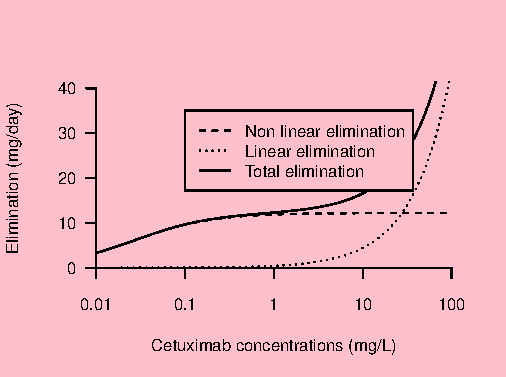
\includegraphics[width=10cm]{images/essai001.pdf}
	\caption[Concentration de cetuximab au cours du temps chez un patient hémodialysé.]{Concentration de cetuximab au cours du temps chez un patient hémodialysé. Les points sont les concentrations observées; la ligne, les concentrations prédites par un modèle à deux compartiments. Dans l'encadré, concentrations prédites vs concentrations observées.}
	\label{fig:18}
\end{figure}

Les estimations des paramètres ne permettaient pas de conclure à une influence du dysfonctionnement rénal ou de l'hémodialyse sur la pharmacocinétique du cetuximab chez ce patient. 
\subsection{Dans le cancer colorectal métastatique (publications~II et III)}
Dans la publication~II, les données de routine de 16 patients (15 traités pour cancer colorectal et 1 pour néoplasie indéterminée) ont été analysées par analyse pharmacocinétique de population. Le modèle décrivant le mieux les données était un modèle à 2 compartiments avec élimination d'ordre 1. Le faible nombre de prises de sang et de patients n'a pas permis d'appliquer un modèle plus complexe.

Le premier objectif de la publication~III était de décrire la pharmacocinétique du cetuximab chez des patients atteints de cancer colorectal métastatique et d'en identifier les sources de variabilité. 

Il s'agissait d'une étude ancillaire d'un essai de phase~II multicentrique (FOLFIRICETUX) qui a évalué la tolérance d'un schéma FOLFIRI (acide folinique, 5-fluorouracile [5-FU] et irinotécan), optimisé en prenant en compte de la pharmacogénomique de l'irinotecan et de la pharmacocinétique du 5-FU et associé au cetuximab administré de façon hebdomadaire. La dose d'irinotecan était adaptée individuellement en fonction du polymorphisme génétique de la partie promotrice d'UGT1A1. Les patients 6/7 avaient une dose inchangée de 180~mg/m$^2$. Les patients 7/7 avaient une dose initiale réduite de 30\% (126~mg/m$^2$). Les patients ayant un autre polymorphisme UGT1A1 avaient une dose initiale de 180~mg/m$^2$ augmentée à chaque cycle de 20\% si la tolérance le permettait jusqu'à une dose maximale de 300~mg/m$^2$. Les doses de 5-FU étaient adaptées au statut de la dihydropyrimidine déshydrogénase (DPD) et à chaque cycle, à la pharmacocinétique du 5-FU.

Entre 2007 et 2009, 96 patients ont été inclus (homme 58 \%, âge moyen : 63 ans [38-80]). Il s'agissait d'un traitement de 2ème ligne chez 82\% des patients. Le cetuximab était administré de façon conventionnelle : une dose de charge de 400~mg/m$^2$ suivie d'injections de 250~mg/m$^2$ toute les semaines. 

Un total de 1322 concentrations sériques de cetuximab a été mesuré avec un nombre moyen de 13 concentrations par patient. Les concentrations sériques résiduelles de cetuximab variaient entre la limite inférieure de quantification (0,75~mg/L) et 300~mg/L.

La pharmacocinétique du cetuximab a été décrite au moyen d'un modèle à 2~compartiments combinant une élimination d'ordre~1 et une élimination d'ordre~0 (Figure~\ref{fig:19}D). Le modèle d'erreur était proportionnel et les 13~concentrations inférieures à la LLOQ ont été censurées. Ce modèle a permis une description satisfaisante des concentrations et notamment des résiduelles très basses (graphiques diagnostiques Figures~\ref{fig:20}-\ref{fig:22}). Le remplacement de l'élimination d'ordre~0 par une élimination de type Michaelis-Menten ne diminuait pas significativement la valeur de la fonction objective. De plus, la valeur de $k_M$ obtenue était inférieure à la LLOQ et n'était donc pas pertinente. Les valeurs de population des cinq paramètres du modèle final étaient correctement estimées avec un CV inférieur à 10\%. Ces valeurs sont présentées dans le Tableau~\textbf{3}. La surface corporelle est apparue comme étant une covariable significative de $V_1$, $V_2$ et $k_0$, ces paramètres augmentant avec sa valeur. L'albuminémie initiale était une covariable significative de $\CL$ : la clairance était d'autant plus importante que l'albuminémie était faible.

\begin{figure}[htbp]
	\centering
		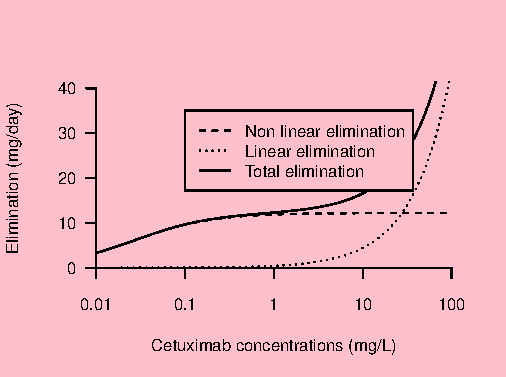
\includegraphics[width=10cm]{images/essai001.pdf}
	\caption[Profils PK d'un patient avec les différents modèles]{Exemples de profils pharmacocinétiques d'un patient obtenus avec les différents modèles testés. \textbf{A} et \textbf{B} : modèles à un et deux compartiments avec élimination d'ordre~1 ($\CL$). \textbf{C} : modèle à deux compartiments avec élimination d'ordre 0 ($k_0$). La meilleure description des concentrations observées est obtenue avec le dernier modèle (\textbf{D}) combinant une élimination d'ordre~0 et une élimination d'ordre~1.}
	\label{fig:19}
\end{figure}

\begin{table}[!ht]
  \centering
  \caption{Valeur estimées des paramètres pharmacocinétique du cetuximab dans l'étude de la publication III.}
    \begin{tabular}{lcccl}
       &  &  &  &  \\
      \hline
      \textbf{} & \textbf{paramètre} & \textbf{s.e.} & \textbf{r.s.e.(\%)} & $p$ \\
      \hline
      \hline
      $V_1$ (L) & 2,96 & 0,12 & 4 &  \\
      $\CL$ (L/jour) & 0,497 & 0,021 & 4 &  \\
      $V_2$ (L) & 4,65 & 0,29 & 6 &  \\
      $Q$ (L/day) & 0,836 & 0,07 & 8 &  \\
      $k_0$ (mg/jour) & 8,71 & 0,84 & 10 &  \\
       &  &  &  &  \\
      $\beta_{V_1,BSA}$ & 0,42 & 0,17 & 41 & 0,015 \\
      $\beta_{V_2,BSA}$ & 0,56 & 0,27 & 49 & 0,039 \\
      $\beta_{k_0,BSA}$ & 1,58 & 0,35 & 22 & 0,0000078 \\
      $\beta_{\CL,Alb}$  & -0,0244 & 0,009 & 37 & 0,0064 \\
       &  &  &  &  \\
      $\omega^2_{V_1}$ & 0,0725 & 0,02 & 28 &  \\
      $\omega^2_{\CL}$ & 0,11 & 0,018 & 17 &  \\
      $\omega^2_{V_2}$ & 0,21 & 0,048 & 23 &  \\
      $\omega^2_{Q}$ & 0,305 & 0,076 & 25 &  \\
      $\omega^2_{k_0}$ & 0,215 & 0,041 & 19 &  \\
       &  &  &  &  \\
      $\sigma^2_{prop}$ & 0,222 & 0,0053 & 2 &  \\
      \hline
    \end{tabular}
  \label{tab:3}
\end{table}
 
\begin{figure}[htbp]
	\centering
		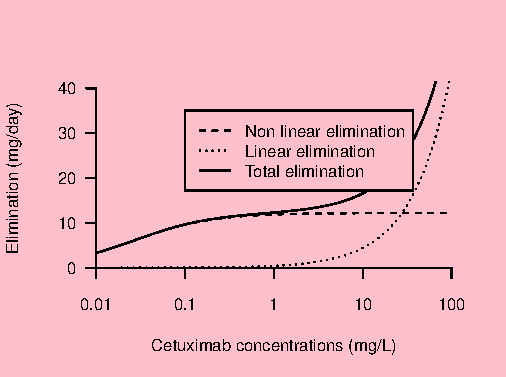
\includegraphics[width=10cm]{images/essai001.pdf}
	\caption{Concentrations de cetuximab observées chez des patients traités pour cancer colorectal métastatique vs. concentrations prédites au moyen d'un modèle à 2 compartiments combinant une élimination d'ordre~1 et une élimination d'ordre~0.}
	\label{fig:20}
\end{figure}

\begin{figure}[htbp]
	\centering
		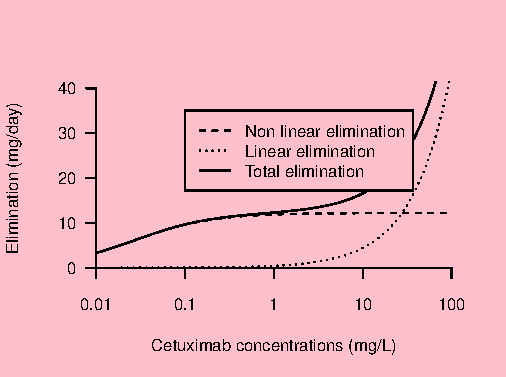
\includegraphics[width=10cm]{images/essai001.pdf}
	\caption{Distribution normalisée des résidus (Normalized prediction distribution errors, NPDE). (A) : distribution (histogramme) et densité de probabilité de la loi normale centrée réduite (courbe). (B) : quantiles des NPDE \textit{vs.} quantiles de la loi normale centrée réduite. En rouge, les 5éme et 95éme percentiles.}
	\label{fig:21}
\end{figure}
\begin{figure}[htbp]
	\centering
		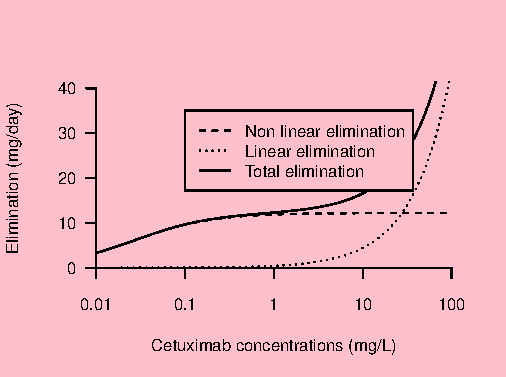
\includegraphics[width=10cm]{images/essai001.pdf}
	\caption{Clairance d'élimination en fonction de la concentration de cetuximab. L'élimination globale du cetuximab (en noir) a été décrite comme la combinaison d'une élimination d'ordre~1 (pointillés) et d'une élimination d'ordre 0 (tirets).}
	\label{fig:22}
\end{figure}

\subsection{Conclusion sur la pharmacocinétique du cetuximab chez l'Homme.}
Les études des publications~II et III ont permis d'obtenir les premières descriptions compartimentales de la pharmacocinétique du cetuximab chez l'Homme dans le cas d'un dysfonctionnement rénal et dans le cas du cancer colorectal métastatique. Le modèle de l'étude~IV était identifiable "grâce" aux pauses thérapeutiques qui ont eu pour conséquence des concentrations résiduelles très basses.

Le modèle utilisé dans l'étude~IV (FOLFIRICETUX) n'est pas significativement meilleur pour décrire les concentrations du patient de l'étude~III (patient hémodialysé) que le modèle à deux compartiments avec élimination d'ordre~1. Dans l'étude~IV, des modèles plus complexes (Michaelis-Menten, TMDD...) ont été testés mais n'étaient pas applicables en raison du nombre insuffisant de données. 

\section{Influence de la pharmacocinétique du cetuximab sur son efficacité (publication~III)}
\subsection{Modélisation pharmacocinétique-pharmacodynamique}
Les connaissances de la relation concentration-effet du cetuximab sont assez limitées 122. Les études concernant l'influence du polymorphisme \textit{FCGR3A}-V158F portent sur la relation dose-effet alors que ce facteur génétique devrait concerner la relation concentration-effet du cetuximab.

La recherche d'un modèle PK-PD stable avec prise en compte ou non des doses de la chimiothérapie associée a été réalisée. Les critères d'efficacité étudiés étaient le critère RECIST, l'ACE et le CA 19.9 ainsi que leurs valeurs relatives par rapport à celles mesurées à l'initiation du traitement. Les modèles TMDD ou PK-PD indirects n'ont pas permis pas de décrire les données pharmacodynamiques, car les paramètres de ces modèles n'étaient pas identifiables. Puisque les données disponibles apparaissaient insuffisantes pour décrire la relation concentration-effet, nous avons choisi de décrire la relation entre concentration et survie sans progression, par approche paramétrique, puis semi-paramétrique.

Dans la cohorte de la publication III, la médiane de survie sans progression (PFS) était de 6,5 mois pour l'ensemble des 96~patients inclus (Figure~\ref{fig:23}). 
\begin{figure}[htbp]
	\centering
		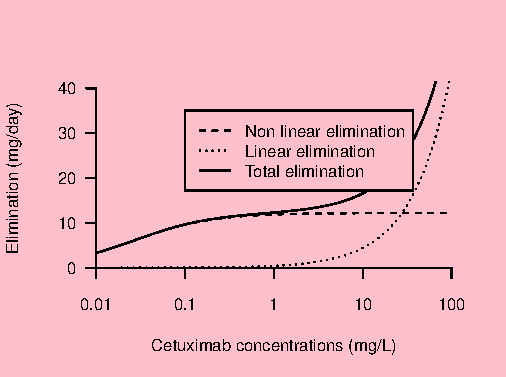
\includegraphics[width=10cm]{images/essai001.pdf}
	\caption[PFS de 96 patients]{Survie sans progression (PFS) des 96 patients traités par cetuximab pour cancer colorectal métastatique.}
	\label{fig:23}
\end{figure}
L'influence sur la PFS des facteurs suivant a été recherchée :
\begin{itemize}
\item exposition au cetuximab et paramètres pharmacocinétiques du cetuximab,
\item facteurs génétiques reliés au cetuximab (statut \textit{KRAS} tumoral et polymorphisme \textit{FCGR3A}-V158F),
\item dose moyenne et nombre d'injections de la chimiothérapie associée,
\item et polymorphismes reliés à cette chimiothérapie.
\end{itemize}
L'approche de modélisation de la PFS utilisée a d'abord été paramétrique, par modèle de Weibull. Le modèle ne permettait cependant pas de décrire de façon satisfaisante les fonctions de survie de sous-groupes de patients. Pour cette raison, nous avons utilisé un modèle de Cox.
\subsection{Influence de l'exposition au cetuximab sur la PFS}
L'$\AUC$ est le meilleur reflet de l'exposition. Cependant, c'est une valeur qui varie au cours du temps : un patient qui a progressé au bout de 6 mois a, à ce moment-là, une $\AUC$ approximativement deux fois supérieure à celle d'un patient qui a progressé (et donc arrêté son traitement) trois mois plus tôt. Un tel paramètre dit "temps-dépendant" peut être intégré dans un modèle de Cox mais son interprétation est difficile. Afin d'obtenir un facteur indépendant du temps, nous avons normalisé l'$\AUC$ par la dose cumulée. Cette $\AUC$ normalisée ($\AUC_n$) avait la dimension d'un temps par unité de volume ([T]$\cdot$[L]$^{-3}$). Pour faciliter l'interprétation, la "clairance globale" qui correspond à l'inverse de l'$\AUC_n$ a été préférée (Volume par unité de temps). La clairance globale a été calculée par l'équation~\ref{eq:11}, l'$\AUC$ étant estimée par approche compartimentale.

Les patients dont la clairance globale était inférieure à la valeur médiane (0,66~L/jour) avaient un temps de progression médian plus long que ceux dont la clairance globale était supérieure à la valeur médiane (8,9 mois vs 3,3 mois) et un risque relatif de progression 2,6 fois moins élevé (p < 5 $\cdot$ 10$^{-5}$) (Figure~\ref{fig:24}). 
\begin{figure}[htbp]
	\centering
		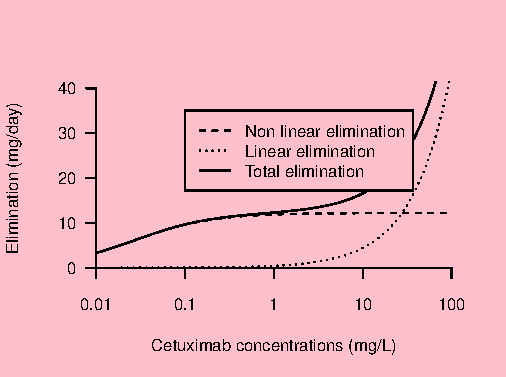
\includegraphics[width=10cm]{images/essai001.pdf}
	\caption{Survie sans progression (PFS) selon la clairance globale médiane (0,66 L/jour). En bleu, le groupe des patients ayant une clairance globale inférieure à la médiane ($n = 48$) ; en rouge le groupe des patients ayant une clairance globale supérieure à la médiane ($n = 48$) ($p < 0,00005$).}
	\label{fig:24}
\end{figure}
Le statut \textit{KRAS} de la tumeur des patients inclus dans l'étude a pu être déterminé rétrospectivement chez 51 patients et la tumeur était non mutée \textit{KRAS} chez 32 d'entre eux. Dans cette étude, la PFS n'était pas influencée par le statut \textit{KRAS} tumoral ($p = 0,66$) (Figure~\ref{fig:25}).
\begin{figure}[htbp]
	\centering
		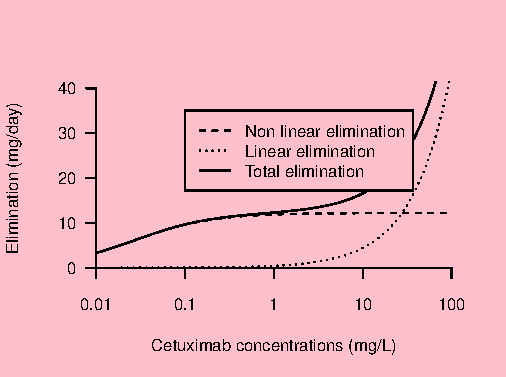
\includegraphics[width=10cm]{images/essai001.pdf}
	\caption{Survie sans progression (PFS) selon le statut \textit{KRAS} tumoral. En bleu, le groupe des patients portant une tumeur non mutés \textit{KRAS} ; en rouge le groupe des patients porteur de tumeur mutée \textit{KRAS} ($p = 0,66$).}
	\label{fig:25}
\end{figure}
Parmi les patients avec une tumeur non mutée \textit{KRAS}, ceux dont la clairance globale était inférieure à la valeur médiane avaient un temps de progression médian plus long que les autres (10,1 mois \textit{vs.} 2,8 mois). Ces patients avaient également un risque de progression 2,8 fois moins élevé ($p = 0,014$). Cette différence n'était pas significative chez les patients ayant une tumeur mutée \textit{KRAS} ($p = 0,21$) (Figure~\ref{fig:26}).
\begin{figure}[htbp]
	\centering
		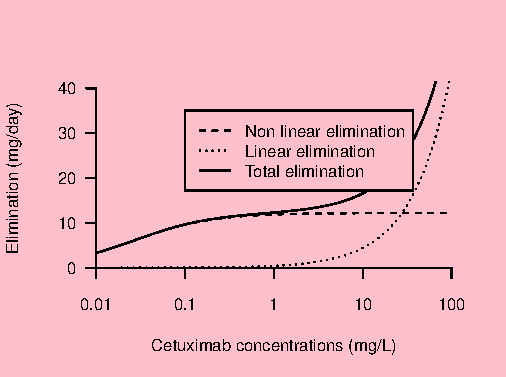
\includegraphics[width=10cm]{images/essai001.pdf}
	\caption{Survie sans progression (PFS) selon la clairance globale médiane. A gauche, le groupe des patients portant une tumeur non mutés \textit{KRAS} ($p = 0,014$); A droite, le groupe des patients porteur de tumeur mutée \textit{KRAS} ($p = 0,21$) - En bleu, le groupe des patients ayant une clairance globale inférieure ou égale à la médiane ; en rouge le groupe des patients ayant une clairance globale supérieure à la médiane.}
	\label{fig:26}
\end{figure} 
Dans cette étude, le polymorphisme \textit{FCGR3A}-V158F n'influençait pas significativement la PFS. Dans le sous-groupe des patients \textit{KRAS} non mutés, six patients étaient homozygotes \textit{FCGR3A}-V/V. Cependant, parmi ces six patients, trois n'ont plus reçu de cetuximab après 6 mois de traitement, ce qui pourrait expliquer la perte de l'avantage d'être \textit{FCGR3A}-V/V (Figure~\ref{fig:27}). 
\begin{figure}[htbp]
	\centering
		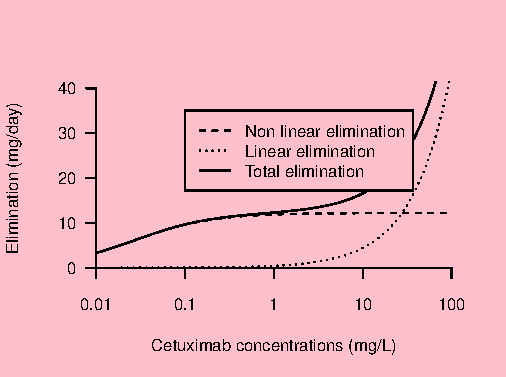
\includegraphics[width=10cm]{images/essai001.pdf}
	\caption{Survie sans progression (PFS) selon le polymorphisme \textit{FCGR3A}-V158F. A gauche, chez les 96 patients ; au milieu, chez les patients porteurs de tumeur non mutée \textit{KRAS} ; à droite, chez les patients porteur de tumeur mutée \textit{KRAS} - En rouge, patients homozygotes \textit{FCGR3A}-V/V ; en bleu, patients porteurs de l'allèle \textit{FCGR3A}-F.}
	\label{fig:27}
\end{figure}
\subsection{Relation entre la toxicité et la PFS}
Nous avons étudié la relation entre la PFS et la présence/absence de toxicité cutanée et une toxicité cutanée supérieure ou non au grade~1, à J7, J14 et J21. La relation entre la PFS et la toxicité cutanée à 21 jours n'était pas significative ($p = 0,077$, Figure~\ref{fig:28}).
Cependant, $k_0$ était significativement plus important chez les patients ayant présenté une toxicité cutanée pendant les 21 premiers jours de traitement ($p = 0,04$). De plus, les valeurs de $k_0$ étaient significativement plus élevées chez les patients ayant présenté un grade de toxicité cutanée supérieur à 1 avant J7 et J14 (respectivement $p = 0,014$ et $p = 0,04$).
\begin{figure}[htbp]
	\centering
		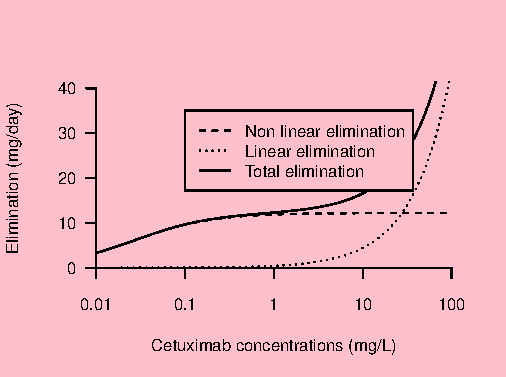
\includegraphics[width=10cm]{images/essai001.pdf}
	\caption{Survie sans progression (PFS) selon la toxicité cutanée à 21 jours. En bleu, groupe des patients n'ayant pas présenté de toxicité cutanée les 21 premiers jours ($n = 21$) ; en rouge le groupe des patients ayant présenté une toxicité cutanée pendant cet intervalle de temps ($n = 69$) ($p = 0,077$).}
	\label{fig:28}
\end{figure}
\subsection{Relation entre les concentrations résiduelles et la PFS}
Pour que l'influence de la pharmacocinétique du cetuximab sur la PFS puisse être estimée le plus tôt possible après l'initiation du traitement en clinique, nous avons étudié la relation entre les concentrations résiduelles avant réinjection et la clairance globale. Les patients du groupe dont la clairance globale était supérieure à la valeur médiane avaient des concentrations résiduelles de l'ordre de 30~mg/L, inférieures à celles de l'autre groupe qui étaient de l'ordre de 60~mg/L (Figure~\ref{fig:29}). La seule étude décrivant la relation concentration-effet in vivo du cetuximab montre que les patients en progression ont des concentrations résiduelles moyennes autour de 30~mg/L alors que les patients stables ou répondeurs ont des concentrations résiduelles moyennes autour de 60 mg/L~\citep{REF122}. Il semblait donc exister un lien entre concentration résiduelle et survie sans progression. 
\begin{figure}[htbp]
	\centering
		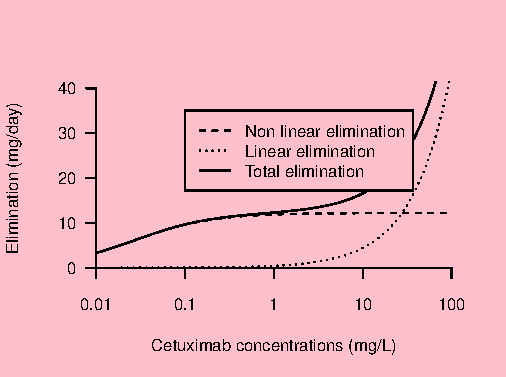
\includegraphics[width=10cm]{images/essai001.pdf}
	\caption{Concentrations résiduelles au cours du temps, en fonction de la clairance globale. En bleu, clairance globale supérieure à la valeur médiane ; En rouge, clairance globale inférieure. Les lignes correspondent aux 5éme, 50éme et 95éme percentiles dans les deux groupes.}
	\label{fig:29}
\end{figure}
Dans notre étude, les concentrations résiduelles les plus nombreuses étaient celles de J14 (avant la troisième injection de cetuximab, $n = 71$) et J28 (avant la cinquième injection, $n = 62$). Après avoir contrôlé la corrélation entre ces concentrations et les valeurs de clairance globale (Figure~\ref{fig:33}), nous avons quantifié leur relation  avec la PFS. Les patients dont la concentration résiduelle à J14 était supérieure à la valeur médiane avaient un risque relatif de progression 1,9 fois plus faible que les autres patients ($p = 0,014$). Les patients dont la concentration résiduelle à J28 était supérieure à la valeur médiane avaient un risque relatif de progression également 1,9 fois plus faible que les autres patients ($p = 0,025$) (Figure~\ref{fig:31}).
\begin{figure}[htbp]
	\centering
		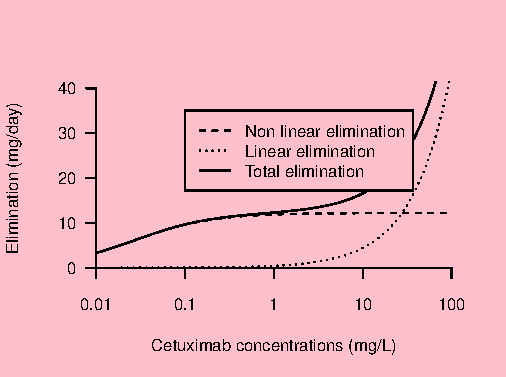
\includegraphics[width=10cm]{images/essai001.pdf}
	\caption{Clairances globales des patients représentées en fonction des concentrations résiduelles à J14 (en haut) et à J28 (en bas). Les courbes représentent des régressions exponentielles, les droites en pointillés représentent le 25éme, 50éme et 75éme percentile des clairances globales.}
	\label{fig:30}
\end{figure}
\begin{figure}[htbp]
	\centering
		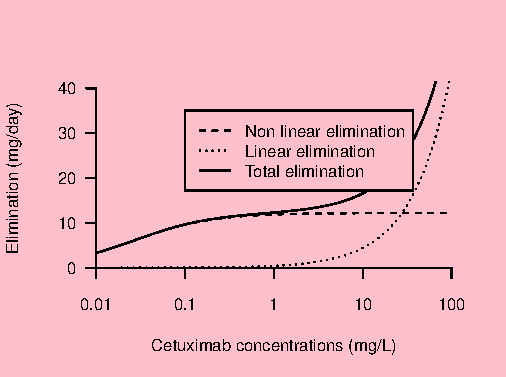
\includegraphics[width=10cm]{images/essai001.pdf}
	\caption{Survie sans progression (PFS) selon la concentration résiduelle de cetuximab avant réinjection. A gauche, concentration résiduelle à J14 ($p = 0,014$) ; a droite, concentration résiduelle à J28 ($p = 0,025$) - En rouge, patients ayant une concentration résiduelle supérieure ou égale à la médiane ; en bleu, patients ayant une concentration résiduelle inférieure à la médiane.}
	\label{fig:31}
\end{figure}
\subsection{Conclusion}
Cette étude a permis de montrer l'influence de l'exposition au cetuximab sur la survie sans progression de patients traités pour cancer colorectal métastatique. Le statut \textit{KRAS} des tumeurs n'était pas directement associé à la survie sans progression. Les deux principales hypothèses pour expliquer cette absence d'influence sont celle d'un manque de puissance statistique due à un faible nombre de patients et celle d'une compensation du manque d'effet du cetuximab chez les porteurs de tumeurs mutées \textit{KRAS} par la chimiothérapie individualisée associée. Le statut \textit{KRAS} a initialement été identifié comme influençant significativement la PFS, sur un nombre moins important de patients~\citep{REF110}. La première hypothèse optant pour un manque de puissance statistique est donc peu plausible. La seconde hypothèse est en revanche plus intéressante. Pour la confirmer, il sera nécessaire de quantifier l'effet des trois médicaments dans un même modèle. Cependant, pour des raisons éthiques, le cetuximab n'est maintenant plus administré aux patients porteurs de tumeurs \textit{KRAS} mutées. Les données de l'étude FOLFIRICETUX sont donc parmi les dernières permettant de quantifier une éventuelle compensation de l'effet des médicaments entre eux. Il serait donc intéressant d'analyser l'influence des concentrations de 5-FU et d'irinotecan sur la relation concentration-effet du cetuximab.

Par ailleurs, le cetuximab a été arrêté relativement tôt chez les six patients \textit{FCGR3A}-V/V, ce qui pourrait expliquer l'absence d'influence significative de ce génotype sur la PFS de nos patients. 

Enfin, nous avons pu mettre en évidence à la fois une relation entre la clairance globale du cetuximab et la concentration sérique résiduelle à J14, et une relation entre cette concentration et la PFS. Ce résultat pourrait permettre d'adapter individuellement la posologie de cetuximab rapidement après l'initiation du traitement si l'intérêt d'une telle procédure est confirmé de façon prospective.

\section{Simulation des concentrations obtenues avec différentes posologies de cetuximab (manuscrit IV)}
\subsection{Contexte}
Dans le cadre du traitement du cancer colorectal métastatique et du cancer ORL, le cetuximab est approuvé pour être administré avec une dose de charge de 400~mg/m$^2$ suivi de perfusions de $250 mg/m^2$ toute les semaines. Cette posologie a montré son efficacité, mais l'intervalle d'injection ($\tau$) n'est pas adapté à celui d'une chimiothérapie concomitante. En effet, pour le cancer colorectal, les injections d'irinotecan ou de 5-fluorouracile (5-FU) sont espacées de deux semaines. Pour le confort du patient, l'injection d'une double dose de cetuximab ($500 mg/m^2$) toute les deux semaines est une posologie de plus en plus utilisée. Cependant, les études visant à justifier l'équivalence de cette posologie avec celle recommandée ne se basent que sur la comparaison des toxicités cutanées ou des réponses cliniques dans des petites cohortes~\citep{REF118}, ~\citep{REF136, REF137, REF138}. Dans le traitement du cancer ORL, la chimiothérapie est administrée toute les trois semaines~\citep{REF105, REF106}. Il est donc également envisagé d'ajuster l'intervalle d'injection du cetuximab à celui de la chimiothérapie dans cette pathologie. 

La variabilité de la pharmacocinétique du cetuximab a été rapportée dans différentes études~\citep{REF68, REF122} ainsi que dans les études des publications~II et III. Une relation entre les concentrations résiduelles de cetuximab et la réponse objective a été décrite précédemment~\citep{REF122}. Cette étude montre que les patients en progression ont des concentrations résiduelles moyennes autour de 30 mg/L alors que les patients stables ou répondeurs ont des concentrations résiduelles moyennes autour de 60 mg/L~\citep{REF122}. Dans la publication III, nous avons également montré que la clairance globale du cetuximab ainsi que la concentration résiduelle à 14 jours, qui en est le reflet, étaient des facteurs reliés significativement avec la survie sans progression (PFS). Il est également reconnu que la pharmacocinétique du cetuximab est dose-dépendante, car elle fait intervenir une élimination saturable~\citep{REF68, REF118, REF123, REF127, REF128}. Cette dose-dépendance rend le choix de posologies équivalentes complexe et peut entraîner une sous-exposition des patients recevant du cetuximab toute les deux ou trois semaines si la posologie est fondée sur une pharmacocinétique considérée comme linéaire.

L'étude de l'équivalence entre différentes posologies de cetuximab doit comparer l'efficacité des traitements, mais doit tout d'abord être fondée sur une bonne description de l'exposition des patients. Nous avons utilisé les paramètres de population obtenus lors de l'analyse de la pharmacocinétique du cetuximab chez des patients traités pour cancer colorectal métastatique (publication~III) pour simuler l'exposition de patients virtuels traités par cetuximab avec différentes posologie, faisant intervenir différentes doses injectées toutes les une, deux ou trois semaines.
\subsection{Simulations}
A l'aide d'une cohorte virtuelle de 1000 patients générés avec les valeurs des paramètres pharmacocinétiques du modèle de la publication~III, nous avons simulé 3 essais cliniques, avec les trois posologies de cetuximab suivantes :
\begin{description}
\item[Posologie~1 :] Dose de charge de 400~mg/m$^2$ suivie de 250~mg/m$^2$ toute les semaines (posologie approuvée).
\item[Posologie~2 :] Dose de 500~mg/m$^2$ de cetuximab toute les deux semaines (posologie déjà utilisée en clinique).
\item[Posologie~3 :] Dose de 750~mg/m$^2$ de cetuximab toute les trois semaines (correspondant à 3$\times$250~mg/m$^2$ toute les semaines)
\end{description}

\subsection{Analyses}
Les trois différents profils pharmacocinétiques obtenus avec les différentes posologies présentaient des différences importantes en termes de concentrations résiduelles (Figure~\ref{fig:32}). La posologie~3 entrainait les concentrations résiduelles de cetuximab les plus faibles, avec une médiane à 48~mg/L et plus de 5\% des patients en deçà de 30~mg/L. Les quantiles des distributions des concentrations résiduelles sont présentés dans le tableau~\ref{tab:4} suivant. 



\begin{table}[htbp]
\caption{Quantiles des distributions des concentrations résiduelles et des $AUC$ cumulées de cetuximab à 84~jours en fonction de la posologie, pour 1000~patients virtuels}
\scriptsize
%\begin{tabularx}{\textwidth}{XX|m{.05\textwidth}m{.05\textwidth}m{.06\textwidth}m{.05\textwidth}m{.05\textwidth}|m{.05\textwidth}m{.05\textwidth}m{.06\textwidth}m{.05\textwidth}m{.05\textwidth}|}
%\begin{tabularx}{\textwidth}{p{2em}p{2em}|XXXXX|XXXXp{2em}|}
%\multicolumn{2}{p{4em}}{\,}	&\multicolumn{5}{|m{.3\textwidth}}{Quantiles des concentrations résiduelles de cetuximab à 84 jours (mg/L)}	
%& \multicolumn{5}{|m{.4\textwidth}|}{Quantiles des $AUC$ cumulées de cetuximab à 84 jours (g/L/jour)} 	\\
%\hline
%\hline
%      Doses (mg/m$^2$) & $\tau$ (semaine) & Mini & 5\% & médiane & 95\% & Maxi & Mini & 5\% & médiane & 95\% & Maxi \\
%      400 - 250 & 1 & 44,6 & 63,1 & 84,3 & 111,9 & 137,6 & 7,8 & 8,9 & 10,4 & 12,4 & 13,8 \\
%      500 & 2 & 30,5 & 42,9 & 63,0 & 88,7 & 115,9 & 7,5 & 8,7 & 10,1 & 12,1 & 13,5 \\
%      750 & 3 & 17,3 & 29,2 & 48,0 & 72,1 & 99,3 & 7,7 & 8,9 & 10,4 & 12,4 & 13,9 \\
%      \hline
%    \end{tabularx}
  \label{tab:4}
\end{table}


\subsection{Conclusions}
Nos résultats objectivent les conséquences potentielles de la non-linéarité du cetuximab sur ses concentrations sériques lors de l'espacement des injections. Bien que les différences observées en termes d'$\AUC$ ne soient pas cliniquement pertinentes, les différences en termes de concentrations résiduelles à l'équilibre sont importantes et leur pertinence doit être étudiée. De plus, l'espacement des injections associé à une augmentation proportionnelle de la dose des perfusions entraine de grands écarts entre les concentrations avant et après injection (pic). Nos résultats donnent des outils pour une adaptation posologique raisonnée lors de l'augmentation des intervalles de perfusion. Nos résultats doivent bien entendu être confirmés par des études pharmacocinétiques prospectives.
\begin{figure}[htbp]
	\centering
		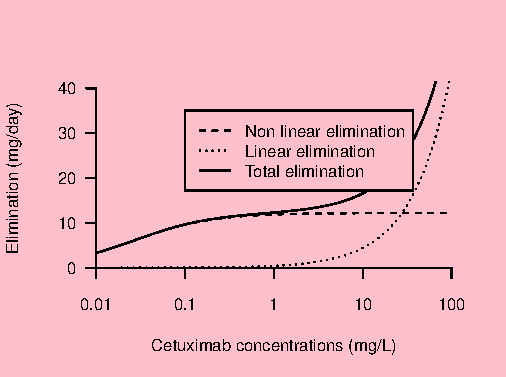
\includegraphics[width=10cm]{images/essai001.pdf}
	\caption{Concentrations de cetuximab simulées avec trois différentes posologies ayant la même dose cumulée sur trois semaines.(Médiane et 90\% \textbf{interval of the patients}) – En rouge, 400~mg/m$^2$ suivie de 250~mg/m$^2$ toute les semaines – En vert, 500~mg/m$^2$ toute les deux semaines – En bleu, 750~mg/m$^2$ toute les trois semaines.}
	\label{fig:32}
\end{figure}
\section{Étude de l'absorption pulmonaire du cetuximab dans un modèle murin (publication~V)}
\subsection{Contexte}
Un des problèmes majeurs associé à l'utilisation du cetuximab est sa toxicité, notamment cutanée, qui limite parfois son emploi 139. Dans le cas du cancer broncho-pulmonaire, son administration par voie inhalée pourrait permettre d'augmenter sa concentration au niveau du site tumoral dans le poumon tout en diminuant sa toxicité systémique. En effet, la présence de FcRn dans le poumon a été montrée~\citep{REF27} et les travaux de Maillet \textit{et al}. ont démontré in vitro la possibilité de nébuliser le cetuximab tout en conservant ses propriétés de fixation à l'EGFR~\citep{REF140}. L'objectif de l'étude était d'analyser par modélisation pharmacocinétique la biodisponibilité du cetuximab administré par nébulisation chez la Souris. L'analyse de ce modèle préclinique était en effet indispensable dans le cadre du développement de cette potentielle nouvelle voie d'administration. Afin de décrire l'évolution des concentrations au cours du temps et d'analyser la biodisponibilité du cetuximab, une modélisation pharmacocinétique a été réalisée à la fois par approches non-compartimentale et compartimentale. 

\subsection{Modèle murin}
Des cellules A431 issues de lignées cellulaires de carcinome épidermoïde cutané ont été obtenues auprès de l'ATCC (American Type Culture Collection). Ces cellules surexpriment de manière constitutive l'EGFR et représentent les cellules de référence pour les études du cetuximab~\citep{REF141}. Dans cette étude, 2,5 $\times 10^6$ cellules ont été instillées par voie endotrachéale chez 13 souris (femelles nude Balb/c de 5 semaines). Le dépôt des cellules marquées par du 99mTc a été suivi par scintigraphie. Six à sept semaines plus tard, les souris ayant développé une tumeur de taille supérieure à 1 mm ont reçu 60 à 80 $\mu$g de cetuximab-Xenofluor750 par voie IV (groupe~IV, $n = 7$) ou par nébulisation dans l'arbre respiratoire (groupe nébulisation, n = 6). Des échantillonnages de sang de 100 à 200 $\mu$L, à H0, H2, H8, J1, J3, J7 et J14 ont permis de mesurer les concentrations sériques de cetuximab par méthode ELISA.
\subsection{Modélisation de la pharmacocinétique}
En ce qui concerne l'approche non-compartimentale, l'$\AUC$ de chaque souris a été estimée par la méthode des trapèzes (équations~\ref{eq:2}~et~\ref{eq:3}). Les moyennes étaient respectivement de 612 et 55,2 h$\times \mu$g/L pour les souris du groupe~IV et nébulisation. La fraction d'$\AUC$ extrapolée n'excédait pas 2,5\% sauf pour une souris du groupe nébulisation (27,15\%). La fraction biodisponible $F$ (équation~\ref{eq:5}), estimée à partir des deux groupes parallèles de souris, était de 9\%. Les moyennes (équations~\ref{eq:7}~et~\ref{eq:8}) étaient respectivement de 59185 et 6745,5 h$^2\dot \mu g/L$ pour les souris du groupe~IV et nébulisation. Le temps de résidence moyen $MRT$ (équation~\ref{eq:6}) était en moyenne de 95 h pour le groupe~IV et de 111,5 h pour le groupe nébulisation. Le temps d'absorption moyen MAT était donc de 34 h. 

L'approche compartimentale a d'abord été réalisée en séparant les groupes. Cependant, la vitesse d'absorption ne permettant pas de bien identifier les paramètres de distribution après nébulisation, les deux voies d'administration ont été analysées de façon conjointe. Le modèle utilisé était bicompartimental avec un compartiment d'absorption pour les souris du groupe nébulisation (équation 19). Les valeurs initiales des paramètres ka et F ont été obtenues par les équations 23 et 5 grâce aux résultats de l'analyse non-compartimentale. Ce modèle a permis une description satisfaisante des concentrations. Les estimations des paramètres et leurs CV interindividuels était $V_1$ = 5,73~mL (6,3\%), $\CL$ = 0,12~mL$\cdot$h$^{-1}$ (13\%) $V_2$ = 9,16~mL (9,6\%), $Q$ = 0,63~mL$\cdot$h$^{-1}$ (16\%) et pour le groupe nébulisation, $k_a$ = 0,04~h$^{-1}$ (25\%). Le poids des souris n'influençait pas significativement les paramètres du modèle.
\begin{figure}[htbp]
	\centering
		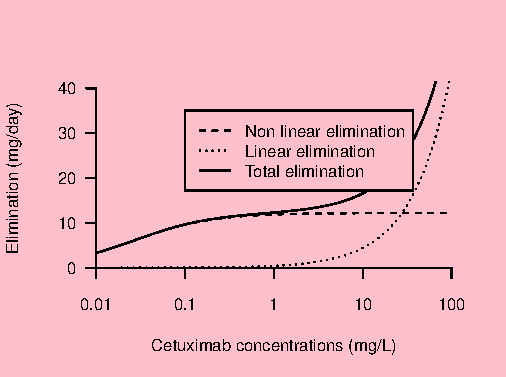
\includegraphics[width=10cm]{images/essai001.pdf}
	\caption{Pharmacocinétique du cetuximab chez la Souris, administré par voie nébulisée (A) et par voie IV (B). Les points représentent les concentrations moyennes ainsi que les écart-types observées pour les souris de chaque groupe. Les traits représentent les concentrations prédites par le modèle final. A noter : l'échelle des concentrations est différente selon la voie d'administration.}
	\label{fig:33}
\end{figure}

\subsection{Conclusions}
La comparaison des profils pharmacocinétiques après administration de cetuximab par nébulisation (Figure~\ref{fig:33}A) et IV (Figure~\ref{fig:33}B) chez la Souris a permis de décrire la phase d'absorption en quantifiant une constante d'absorption $k_a$ et une fraction absorbée $F$. La bonne description de cette absorption par une constante d'ordre~1 suggère que le FcRn pulmonaire, qui est vraisemblablement le principal acteur du passage des IgG à travers la barrière alvéolo-capillaire~\citep{REF27}, n'est pas saturé chez la Souris aux doses utilisées.

Dans le cas d'un cancer broncho-pulmonaire, l'effet recherché du cetuximab est locorégional. La faible fraction absorbée ($F$ = 9 à 11\%) et la persistance du cetuximab dans le poumon ($MAT$ de 34 h et persistance du marquage pulmonaire par le Xenofluor) suggèrent une bonne exposition des tissus pathologiques après nébulisation. Dans le modèle murin utilisé, l'administration de cetuximab en aérosol a permis une régression significative de la masse tumorale (Publication V, Figure 5A).
 
%%%%%%%%%%%%%%%%%%%%%%%%%%%%%%%%%%%%%%%%%%%%%%%%%%%%%%%%%%%%%%%%%%%%%
%DISCUSSION :
\chapter{Discussion}
Le développement et la validation de la méthode de dosage de cetuximab par technique ELISA ont permis d'obtenir des mesures fiables des concentrations sériques de cetuximab. Un certain nombre de techniques de dosage du cetuximab dans le sérum sont mentionnées dans la littérature mais aucune n'est décrite de façon détaillée. Il ne nous est donc pas possible de comparer les performances de notre technique avec celles rapportées par d'autres équipes. L'utilisation d'une protéine recombinante produite dans le cadre d'une collaboration régionale implique que nos résultats devront, à terme, être comparés avec ceux obtenus par d'autres techniques ELISA. Les concentrations cibles données dans la publication~IV sont donc à interpréter avec prudence si une autre technique est utilisée. Toutefois, ceci ne modifie pas la conclusion principale de ce travail, qui est que le suivi thérapeutique des concentrations sériques de cetuximab chez les patients traités pour cancer colorectal métastatique pourrait être utile. 

De façon générale, l'erreur résiduelle d'un modèle pharmacocinétique de population décrivant des concentrations mesurées par une méthode ELISA est décrite de façon satisfaisante par un modèle mixte additif et proportionnel~\citep{REF68, REF73}. La partie additive du modèle prend en compte le bruit de fond de la technique, tandis que la partie proportionnelle suit la portion linéaire croissante de la courbe de calibration. En deçà de la limite basse de quantification de la technique (LLOQ), il est recommandé de censurer la valeur de la concentration, pour permettre une meilleur estimation de l'élimination à concentration basse~\citep{REF142}. Cette censure, bien que justifiée pour des raisons analytiques, peut poser problème lors du choix du modèle structural~\citep{REF143}. Dans l'étude pharmacocinétique de la publication~III, qui prenait en compte la censure des concentrations inférieures à la LLOQ, un problème d'identifiabilité entre la variabilité interindividuelle de $k_0$ et la partie additive du modèle d'erreur résiduelle a été rencontré : la variabilité de l'erreur résiduelle additive était très proche de zéro et la variabilité de $k_0$ présentait un important "shrinkage" (variabilité interindividuelle estimée trop élevée). Le problème a été contourné en utilisant un modèle d'erreur résiduelle proportionnel (équation~\ref{eq:51}). La variabilité interindividuelle de $k_0$ correspondait donc également au « bruit de fond » de la technique analytique. Dans les études publiées, les modèles d'erreur utilisés pour décrire l'élimination des anti-EGFR étaient de type mixte additif et proportionnel~\citep{REF68, REF73}. Cependant, les concentrations inférieures aux limites de quantification des techniques de dosage utilisées n'étaient pas censurées. Dans l'étude pharmacocinétique de la publication~III, les concentrations basses étaient très informatives pour la quantification de l'élimination saturable. Supprimer les concentrations inférieures à la LLOQ n'est pas recommandé ; ceci serait une perte d'information~\citep{REF142}. Le problème d'identifiabilité rencontré ici pourrait sans doute être résolu en adaptant le modèle d'erreur résiduelle au profil de la courbe de calibration de la technique de dosage. Dans ce modèle, les concentrations proches des limites basse et haute de quantification seraient prises en compte par une pondération moins importante que celle des concentrations issues de la partie linéaire de la courbe de calibration.

Les résultats de la modélisation individuelle du cetuximab réalisée chez un patient insuffisant rénal dialysé ont montré que la pharmacocinétique de cet anticorps était comparable à celle décrite chez des patients sans insuffisance rénale. La pharmacocinétique du cetuximab ne semble donc être influencée ni par un dysfonctionnement rénal ni par une dialyse chronique, bien que ces résultats doivent être confirmés sur un plus grand nombre de sujets. Les injections étaient trop rapprochées pour identifier une élimination saturable chez ce patient, bien que les concentrations observées entre le 49ème et le 56ème jour aient un profil comparable à celle des patients de la publication~III.

La publication~III confirme la non-linéarité de la pharmacocinétique du cetuximab décrite par Dirks~\textit{et al.}, bien qu'ils aient décrit l'ensemble de l'élimination comme étant de type Michaelis-Menten~\citep{REF68}. Notre modèle semble plus mécanistique car il permet la description des deux types d'éliminations connues pour les anticorps thérapeutiques. Cette approche a déjà été appliquée par Ma~\textit{et al.} au panitumumab~\citep{REF73} et par Kuester~\textit{et al.} au matuzumab~\citep{REF129}. Dans notre travail, l'élimination non saturable (\gls{CL}) était reliée à l'albuminémie, ce qui pourrait correspondre à l'implication du FcRn dans ce mode d'élimination. En effet, un FcRn avec une moins bonne affinité pour la portion Fc des anticorps et pour l'albumine et$/$ou un FcRn présent en plus petite quantité va recycler une plus faible quantité d'anticorps et d'albumine. La clairance de ces deux protéines sera donc augmentée. Le paramètre $k_0$ étant relié à la surface corporelle (BSA) et à la toxicité cutanée, l'élimination saturable pourrait quant à elle décrire l'élimination spécifique du cetuximab, consécutive à sa fixation sur l'EGFR, présent en quantité importante sur les épithéliums. Une publication récente présente des résultats in vitro de mesure de la constante de dissociation $K_d = k_{off}/k_{on}$ de trois anticorps anti-EGFR (cetuximab, panitumumab et matuzumab)~\citep{REF144}. Cette étude rapporte des $K_d$ très faibles pour les trois anticorps, ce qui justifie une simplification d'un modèle de type TMDD en un modèle intégrant une élimination de type Michaelis-Menten ou même une élimination d'ordre~0 ($k_0$) pour décrire l'élimination spécifique d'un anticorps anti-EGFR. Cependant, cette simplification ne permet pas de prendre en compte les variations de quantité de cible de l'anticorps au cours du temps. L'explication de ces variations est pourtant indispensable à une bonne description de l'élimination spécifique de l'anticorps et donc à la description de sa relation concentration-effet. Dans le cadre de cette thèse, toutes les tentatives de description de la pharmacocinétique du cetuximab (publication~III) par des modèles plus complexes (approches TMDD notamment), prenant en compte une variation de la quantité de cible, étaient tous sur-paramétrés.

Compte tenu de cette non linéarité, une modification de la posologie telle qu'une augmentation de l'intervalle de temps entre les injections doit reposer sur une simulation pharmacocinétique. Nous avons utilisé le modèle pharmacocinétique décrit dans la publication~III pour simuler les concentrations attendues avec différentes doses de perfusion pour des intervalles d'une, deux et trois semaines (manuscrit~IV). Les résultats montrent que le doublement ou le triplement de la dose sont insuffisants pour maintenir des concentrations résiduelles comparables lorsque l'intervalle entre deux perfusions est doublé ou triplé. Bien que significativement différente en raison du grand nombre de patients simulés, la distribution des valeurs d'\gls{AUC} pour les posologies ayant la même dose cumulée sur trois semaine mais des intervalles d'injection différents, ne montre pas de différences d'échelle aussi importante que les concentrations résiduelles. Néanmoins, ces résultats préliminaires justifient un suivi minutieux des concentrations de cetuximab dans les études testant un espacement des perfusions.  

Pour réaliser une modélisation de type TMDD du cetuximab et de l'EGFR, il faudrait disposer d'une estimation des quantités d'EGFR libres et/ou liées au cetuximab, mais également de la proportion d'EGFR présente sur les cellules cancéreuses, et sur les cellules saines (épithéliums et endothéliums entre autres). Cependant, la difficulté de quantification de l'EGFR \textit{in vivo} et sa double localisation sur les tissus tumoraux et sains rendent cette modélisation difficile. Le critère RECIST est un indicateur efficace de la réponse d'un patient, mais c'est un critère composite qui présente une forte variabilité interindividuelle. La description de son évolution par approche PK-PD s'est révélée impossible. Une modélisation reposant sur un modèle de type TMDD aurait eu pour conséquences une sur-paramétrisation compte tenu des données disponibles. L'utilisation d'autres biomarqueurs tels que le CA19.9 ou l'ACE présentaient les mêmes types de limitations. 

De plus, dans l'étude de la publication~III, les doses de chimiothérapie associée étaient ajustées individuellement. Cette influence a été recherchée sans succès dans les essais de modélisation PK-PD du cetuximab et dans l'étude de la survie sans progression, par le biais de la dose cumulée ou du nombre d'injections. Cependant, il semble logique de penser que l'effet de cette chimiothérapie ne doit pas être séparé de la relation dose-concentration-effet du cetuximab dans le cancer colorectal. Il faudrait donc modéliser de façon conjointe la relation dose-concentration-effet du cetuximab, de l'irinotecan et du \gls{5FU} pour quantifier l'influence de l'exposition à ces trois médicaments. Ce modèle entièrement paramétrique pourrait permettre de comparer par simulation l'intérêt de différentes posologies d'irinotecan, de \gls{5FU} et de cetuximab, lors de leur association. 

Les résultats de la publication~III montrent que la survie sans progression (PFS) n'est pas influencée par l'élimination saturable ou l'élimination non-saturable du cetuximab, mais par la clairance globale estimée sur le temps avant progression, c'est-à-dire, la combinaison de \gls{CL} et $k_0$. Ce ne sont donc pas les phénomènes d'élimination mais l'exposition au cetuximab qui en résulte qui influence la PFS des patients traités.

Une bonne estimation de la clairance globale nécessite une étude de la pharmacocinétique pendant un temps assez long. Si cela est possible rétrospectivement à partir des données d'une étude clinique comme celle-ci, cela n'est pas réalisable couramment en clinique. Les travaux de la publication~III montrent que la concentration résiduelle de cetuximab à J14 est un bon reflet de la clairance globale et est reliée à la survie sans progression. Cette concentration résiduelle à J14 pourrait donc être utilisée en clinique comme indicateur précoce de la clairance globale et donc de la survie sans progression. Après confirmation par une étude prospective, les patients ayant une concentration résiduelle trop basse pourraient alors bénéficier d'un ajustement précoce de dose pour optimiser leur réponse clinique.

Une relation entre la concentration résiduelle et la réponse a été rapportée pour un autre anticorps monoclonal antitumoral indiqué dans les tumeurs solides, le trastuzumab~\citep{REF145} Notre approche pourrait donc s'appliquer à d'autres anticorps antitumoraux.

La modélisation de la pharmacocinétique du cetuximab administré par voie pulmonaire chez la Souris a permis la description de son absorption. Cette faible biodisponibilité (F proche de 10 $\%$) est un élément positif car il montre une faible exposition systémique (donc un faible risque d'effets indésirables tels que les effets cutanés) et devrait correspondre à une forte exposition loco-régionale (pulmonaire). Cette accumulation du cetuximab dans le poumon est confirmée par les données d'imagerie obtenues avec le cetuximab marqué au Xenofluor. Ces résultats encourageants ont incité l'équipe INSERM U618 à lancer une nouvelle étude équivalente chez le Singe. Cette étude est actuellement en cours d'analyse.

Notre travail montre que, comme les autres anticorps thérapeutiques, le cetuximab a une grande variabilité pharmacocinétique interindividuelle. Ceci justifie la recherche des sources de cette variabilité pharmacocinétique et nécessite d'étudier l'impact de cette variabilité sur la réponse au traitement, c'est-à-dire la relation concentration-effet. Ces deux domaines d'étude reposent sur une description quantitative précise de la pharmacocinétique, ce qui est un défi compte tenu de la complexité des phénomènes impliqués dans le devenir des anticorps dans l'organisme. Nous avons pu appliquer avec succès un modèle bicompartimental avec ou sans absorption d'ordre~1 au modèle murin, un modèle bicompartimental "simple" au patient en insuffisance rénale traité par hémodialyse et un modèle avec élimination mixte (non saturable et saturée) aux patients traités pour cancer colorectal métastatique. Ce dernier modèle nous a permis d'identifier des facteurs de variabilité pharmacocinétique associés au traitement de cette pathologie. Il semble cependant nécessaire de développer des modèles plus complexes, faisant intervenir éventuellement la quantité d'antigène-cible et/ou l'influence des  médicaments associés, pour identifier plus précisément l'ensemble des facteurs de variabilité pharmacocinétique. Le modèle obtenu pourrait permettre de mieux prédire la pharmacocinétique du cetuximab et ainsi d'argumenter de façon plus pertinente une optimisation individuelle de sa posologie. Un modèle pharmacocinétique mieux ajusté aux données pourrait également permettre d'améliorer l'étude de la relation concentration-réponse et donc de permettre, si un biomarqueur pertinent est disponible, d'étudier les sources individuelles de variabilité de sensibilité au traitement, tels que les polymorphismes des récepteurs Fc$\gamma$R.
 
\end{spacing}
%%%%%%%%%%%%%%%%%%%%%%%%%%%%%%%%%%%%%%%%%%%%%%%%%%%%%%%%%%%%%%%%%%%%%
%La biblio :
\addcontentsline{toc}{chapter}{Bibliographie}
%\bibliographystyle{apalike-fr}  % Auteur Date 
\bibliographystyle{unsrt}      % Numero
\bibliography{./Biblio/BiblioThese2}
%%%%%%%%%%%%%%%%%%%%%%%%%%%%%%%%%%%%%%%%%%%%%%%%%%%%%%%%%%%%%%%%%%%%%
\listoftables 
\listoffigures 
\printglossaries

%%%%%%%%%%%%%%%%%%%%%%%%%%%%%%%%%%%%%%%%%%%%%%%%%%%%%%%%%%%%%%%%%%%%%
%Les glossaire :
\addcontentsline{toc}{chapter}{Glossaire}
\chapter*{Abréviations}
%\addcontentsline{toc}{chapter}{Abréviations}
%\markright{\MakeUppercase{Abréviations}}
\begin{tabularx}{30em}{X X}
5-FU & 5-fluorouracile\\
$\alpha$ & 	Pente de décroissance de la phase de distribution d'un modèle bi-compartimental\\
ADCC & 	Cytotoxicité à médiation cellulaire dépendante des anticorps (\textit{Antibody-dependent cell-mediated cytotoxicity})\\
AMM & 	Autorisation de mise sur le marché\\
$\AUC$ & 	Aire sous la courbe des concentrations en fonction du temps (\textit{Area under the concentration-time versus curve})\\
$\AUMC$ & 	Moment d'ordre 1 de la courbe des concentrations en fonction du temps (\textit{Area under the first moment of the concentration versus time curve})\\
$\AUC_n$ & 	AUC normalisée à la dose\\
ATI & 	Anticorps anti-infliximab (\textit{Antibodies toward infliximab})\\
$\beta$ & 	Pente de décroissance de la phase d'élimination d'un modèle bi-compartimental\\
$C$ & 	Concentration de médicament\\
$C_{max}$ & 	Concentration maximale du médicament observée après une dose unique\\
$\CL$ & 	Clairance systémique\\
$C_n$ & 	Dernière concentration mesurée\\
CRP & 	Protéine C-réactive (\textit{C-reactive protein})\\
$D$ & 	Dose\\
Da & 	Dalton : Unité de masse atomique $\approx  1,66054\times 10^{-27} kg$\\
DPD & 	Dihydropyrimidine déshydrogénase\\
EGF & 	Facteur de croissance épidermique (\textit{Epidermal growth factor})\\
EGFR & 	Récepteur au facteur de croissance épidermique. Aussi appelé HER1 ou c-ErbB-1 (\textit{Epidermal growth factor receptor})\\
ELISA & 	\textit{Enzyme-linked immunosorbent assay}\\
ERK & 	\textit{Extracellular signal-regulated kinase}\\
EV & 	Extra-vasculaire (administration)\\
$F$ & 	Fraction absorbée après administration extravasculaire\\
Fc$\gamma$RIIIA & 	Récepteur membranaire de la portion Fc des immunoglobulines G. Aussi appelé CD16a\\
\textit{FCGR3A} & 	Gène codant Fc$\gamma$RIIIA\\
FDA & 	Food and Drug Administration\\
Ig & 	Immunoglobuline. Chez l'Homme, elles sont de classe A, D, E, G ou M : IgA, IgD, IgE, IgG ou IgM \\
IV & 	Intra-veineuse (administration)\\
JAK2 & 	Janus Kinase 2\\
$k_{10}$ & 	Constante d'élimination d'ordre~1 également notée $k_e$\\
$k_{12}$ & 	Constante de transfert d'ordre~1 du compartiment~1 vers le compartiment~2\\
$k_{21}$ & 	Constante de transfert d'ordre~1 du compartiment~2 vers le compartiment~1\\
$k_a$ & 	Constante d'absorption d'ordre~1 également notée $k_{01}$\\
$k_t$ & 	Constante de transfert d'ordre~1 entre compartiments de transit\\
LC-MS/MS & 	Chromatographie en phase liquide couplée à une spectrométrie de masse en tandem (\textit{Liquid chromatography coupled to tandem mass spectrometry})\\
$\mu$ & 	Moyenne\\
$\MAT$ & 	Temps d'absorption moyen (\textit{Mean absorption time})\\
MAPK & 	Kinases activées par des agents mitogènes (\textit{Mitogen-activated protein kinase})\\
MM & 	Michaelis-Menten\\
$\MRT$ & 	Temps de résidence moyen (\textit{Mean residence time})\\
NPDE & 	Distribution normalisée des résidus (\textit{Normalized prediction distribution error})\\
OS & 	Survie globale (Overall survival)\\
PFS & 	Survie sans progression (\textit{Progression-free survival})\\
PI3K & 	Phosphatidylinositol 3-kinase (Phosphoinositide 3-kinase)\\
PK & 	Pharmacocinétique (\textit{Pharmacokinetics})\\
PK-PD & 	Relation pharmacocinétique-pharmacodynamique (\textit{Pharmacokinetic-Pharmacodynamic relationship})\\
$Q$ & 	Clairance de distribution, également notée $CL_2$\\
$\sigma$ & 	Écart-type\\
SC & 	Sous-cutanée (administration)\\
STAT3 & 	\textit{Signal transducer and activator of transcription 3}\\
$\tau$ & 	Intervalle de temps entre deux administrations\\
$T$ & 	Durée de la perfusion\\
TGF$\alpha$ & 	Facteur de croissance transformant alpha (\textit{Transforming growth factor-alpha})\\
TK & 	Tyrosine kinase \\
$T_{max}$ & 	Temps correspondant à la concentration maximale $C_{max}$ dans le cas d'une administration unique\\
TMDD & 	Élimination liée à la cible (\textit{Target-mediated drug disposition})\\
TV & 	Valeur typique d'un paramètre (\textit{Typical value})\\
$t_{1/2}$ & 	Demi-vie dans le cas d'un modèle bi-compartimental ; $t_{1/2}\alpha$ = demi-vie de distribution ; $t_{1/2}\beta$ = demi-vie d'élimination.\\
$V$ & 	Volume de distribution ($V_{SS}$, $V_1$, $V_2$)\\
\end{tabularx}
 
%%%%%%%%%%%%%%%%%%%%%%%%%%%%%%%%%%%%%%%%%%%%%%%%%%%%%%%%%%%%%%%%%%%%%
%Articles
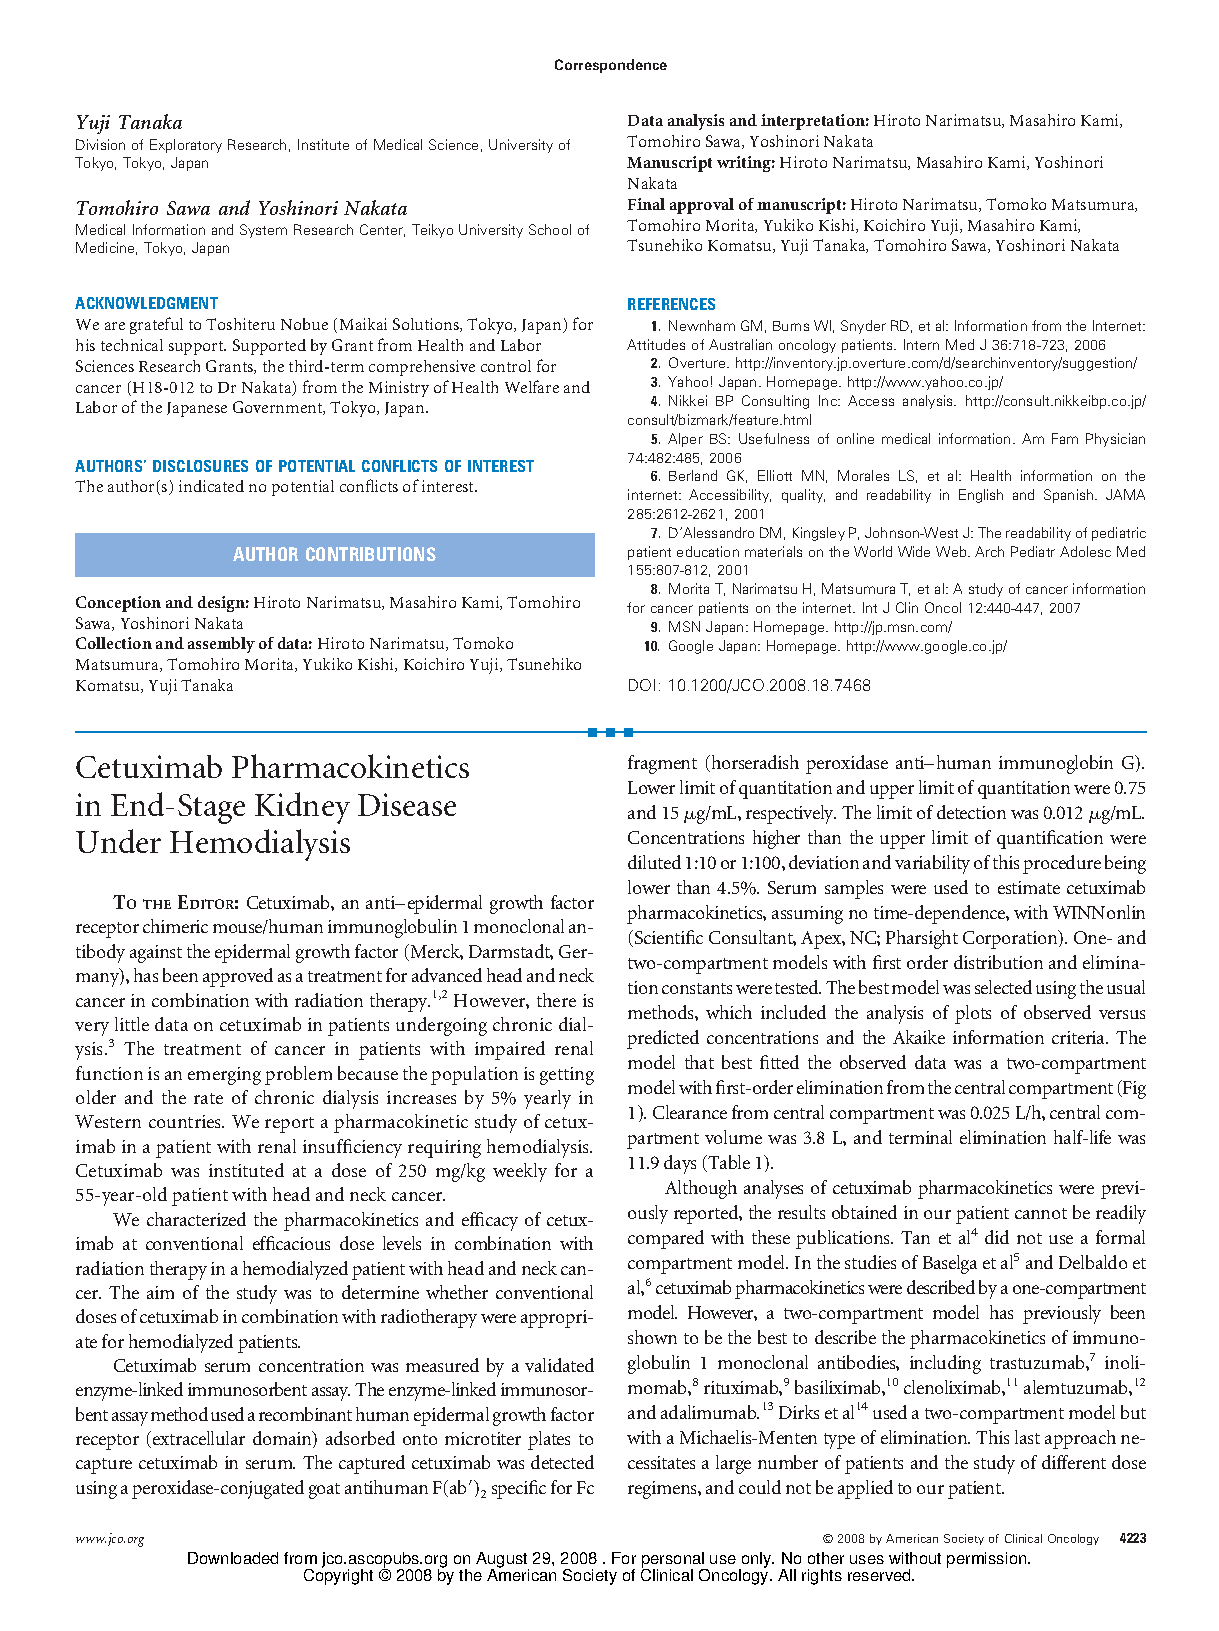
\includepdf[pages=1-3]{./articles/Thariat.pdf}
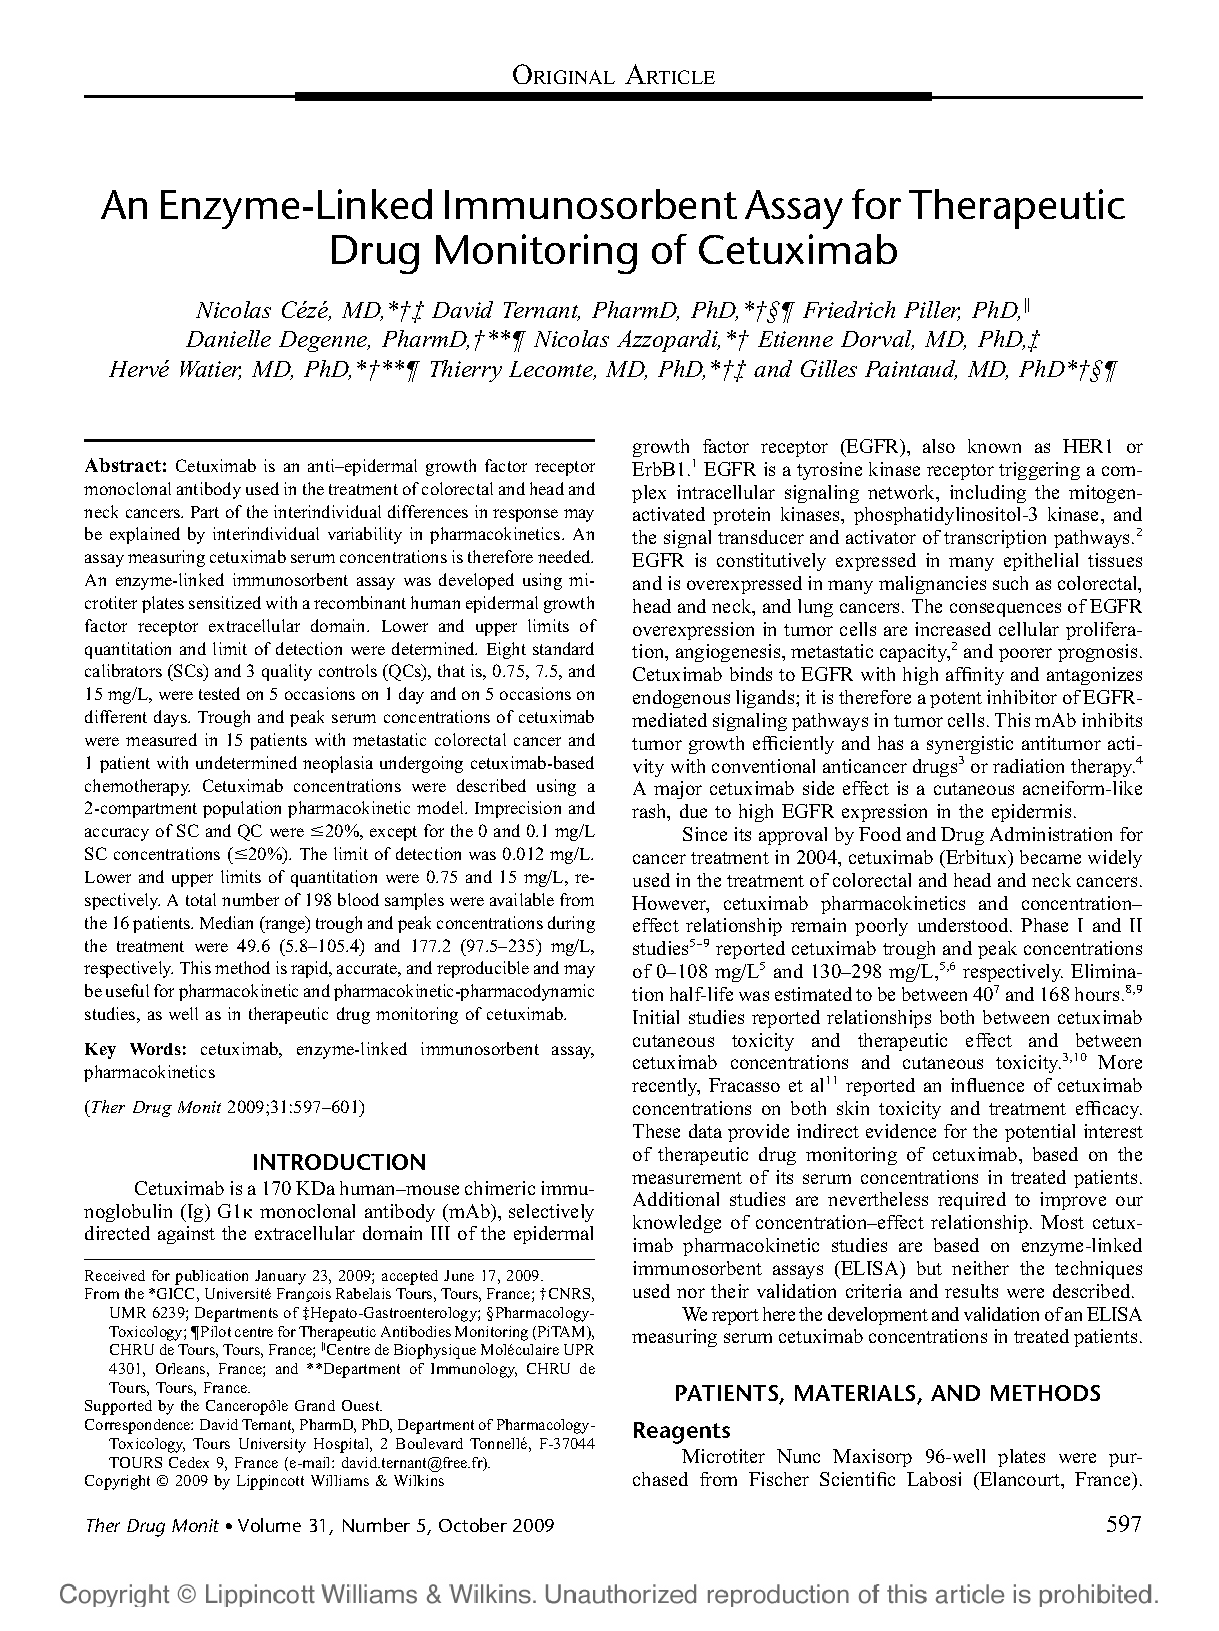
\includepdf[pages=1-5]{./articles/Ceze.pdf}
%%%%%%%%%%%%%%%%%%%%%%%%%%%%%%%%%%%%%%%%%%%%%%%%%%%%%%%%%%%%%%%%%%%%%
%La page de dos :
\thispagestyle{empty}
\thispagestyle{empty}
\setmarginsrb{20mm}{20mm}{25mm}{0mm}{0mm}{0mm}{0mm}{0mm}
\begin{tabular}{ p{3cm} p{9cm} p{3cm}}
		\begin{minipage}{3cm}
			
\includegraphics[width=3cm]{./images/pucvl.png} 
		\end{minipage}
	&
		\begin{minipage}{9cm}
			\begin{center}
				\textbf{Apport de la modélisation pharmacocinétique à l'étude de la variabilité de réponse aux anticorps monoclonaux antitumoraux : Application au cetuximab}

Nicolas AZZOPARDI
			\end{center}
		\end{minipage}
	&
		\begin{minipage}{3cm}
			
\includegraphics[width=3cm]{./images/ufr.png} 
		\end{minipage}
\end{tabular}
\vspace{1cm}
\begin{minipage}{16cm}
\section*{Résumé :}
Les anticorps monoclonaux ont révolutionné le traitement de nombreuses pathologies. Cependant, leur pharmacocinétique (PK) et l'influence de leur concentration sur la réponse clinique restent mal connues. Nous avons étudié les sources de variabilité interindividuelle de la PK du cetuximab, un anticorps anti-EGFR, ainsi que l'influence de l'exposition à cet anticorps sur la réponse. Nous avons validé une méthode ELISA de dosage du cetuximab. Dans un modèle murin, nous avons étudié l'absorption pulmonaire du cetuximab. Nous avons étudié la PK du cetuximab chez un patient hémodialysé. Nous avons décrit la PK du cetuximab chez des patients traités pour cancer colorectal métastatique, à l'aide d'un modèle combinant des éliminations d'ordre~0 et 1. Enfin, nous avons identifié la clairance globale du cetuximab, paramètre pouvant être estimé précocement par la concentration résiduelle à J14, comme un facteur influençant la survie sans progression des patients. Nos travaux montrent qu'une description de la PK d'un anticorps par approche compartimentale permet d'identifier les sources de variabilité et d'étudier l'impact de la PK sur la réponse clinique.
\paragraph*{Mots clés :} anticorps monoclonaux, cetuximab, ELISA, pharmacocinétique, relation dose-réponse, survie sans progression, polymorphisme génétique, récepteurs Fc
\vspace{1cm}
\section*{Abstract :}
Monoclonal antibodies have profoundly modified the treatment of many diseases. However, their pharmacokinetics (PK) and the influence of their concentrations on the clinical response are poorly known. We studied the sources of the interindividual variability of PK of cetuximab, an anti-EGFR, and the influence of the exposure to this antibody on the response. We validated an ELISA technique to measure cetuximab concentrations. We studied the pulmonary absorption of cetuximab in a murine model. We studied cetuximab PK in a hemodialysed patient. In metastatic colorectal cancer patients, we described cetuximab PK with the help of a model combining zero- and first-order eliminations. Finally, we identified the global clearance of cetuximab, a parameter which can be estimated by residual concentration on day 14, as a factor influencing progression-free survival of the patients. Our work shows that the description of the PK of an antibody by compartmental approach allows to identify sources of variability and to study the impact of PK on the clinical response.
\paragraph*{Keywords :} monoclonal antibodies, cetuximab, ELISA, pharmacokinetics, dose-response relationship, genetic polymorphism, Fc receptors
\end{minipage}
\end{document}
